\documentclass[a4paper,11pt]{article}
\pdfoutput=1
\usepackage{jheppub}
\usepackage[T1]{fontenc}
\usepackage{bm}
\usepackage{booktabs}
\usepackage{tikz}
\usetikzlibrary{decorations.pathmorphing,arrows.meta}

% ---------------------------------------------------------------- notation
\newcommand{\x}{\bm{x}}
\newcommand{\y}{\bm{y}}
\newcommand{\z}{\bm{z}}
\newcommand{\w}{\bm{w}}
\newcommand{\cc}{\bm{c}}
\newcommand{\bx}{\bar{\bm{x}}}
\newcommand{\by}{\bar{\bm{y}}}
\newcommand{\bz}{\bar{\bm{z}}}
\newcommand{\yp}{\bm{y}'}
\newcommand{\xp}{\bm{x}'}
\newcommand{\byp}{\bar{\bm{y}}'}
\newcommand{\bxp}{\bar{\bm{x}}'}
\newcommand{\R}{\bm{R}}
\newcommand{\Y}{\bm{Y}}
\newcommand{\X}{\bm{X}}
\newcommand{\Rt}{\widetilde{\bm{R}}}
\newcommand{\bR}{\bar{\bm{R}}}
\newcommand{\bY}{\bar{\bm{Y}}}
\newcommand{\bX}{\bar{\bm{X}}}
\newcommand{\bRt}{\bar{\widetilde{\bm{R}}}}
\newcommand{\kk}{\bm{k}}
\newcommand{\pp}{\bm{p}}
\newcommand{\qq}{\bm{q}}
\newcommand{\lv}{\bm{l}}
\newcommand{\kt}{\widetilde{\bm{k}}}
\newcommand{\pt}{\widetilde{\bm{p}}}
\newcommand{\ktq}{\widetilde{\bm{k}}_q}
\newcommand{\ptq}{\widetilde{\bm{p}}_q}
\newcommand{\kap}{\bm{\kappa}}
\newcommand{\rhov}{\bm{\rho}}
\newcommand{\PP}{\bm{P}}
\newcommand{\KK}{\bm{K}}
\newcommand{\ef}{\epsilon_f}
\newcommand{\eft}{\tilde{\epsilon}_f}
\newcommand{\of}{\omega_f}
\newcommand{\oft}{\tilde{\omega}_f}
\newcommand{\Ef}{E_f}
\newcommand{\mf}{m_f}
\newcommand{\zb}{(1-\zeta)}
\newcommand{\eb}{(1-\eta)}
\newcommand{\cG}{\mathcal{G}}
\newcommand{\cA}{\mathcal{A}}
\newcommand{\cM}{\mathcal{M}}
\newcommand{\Amp}{\mathsf{A}}
\newcommand{\cH}{\mathcal{H}}
\newcommand{\cW}{\mathcal{W}}
\newcommand{\cS}{\mathcal{S}}
\newcommand{\cD}{\mathcal{D}}
\newcommand{\cQ}{\mathcal{Q}}
\newcommand{\cP}{\mathcal{P}}
\newcommand{\tG}{\widetilde{\mathcal{G}}}
\newcommand{\tA}{\widetilde{\mathcal{A}}}
\newcommand{\tM}{\widetilde{\mathcal{M}}}
\newcommand{\tH}{\widetilde{\mathcal{H}}}
\newcommand{\tPsi}{\widetilde{\Psi}}
\newcommand{\tF}{\widetilde{F}}
\newcommand{\bF}{\bar{F}}
\newcommand{\btF}{\bar{\widetilde{F}}}
\newcommand{\aem}{\alpha_{\rm em}}
\newcommand{\as}{\alpha_s}
\newcommand{\Nc}{N_c}
\newcommand{\CF}{C_F}
\newcommand{\qqbar}{q\bar q}
\newcommand{\qqg}{q\bar q g}
\newcommand{\ee}{\varepsilon}
\newcommand{\re}{{\rm Re}\,}
\newcommand{\tr}{{\rm tr}}
\newcommand{\dd}{{\rm d}}
\newcommand{\order}[1]{\mathcal{O}(#1)}
\newcommand{\gT}{\gamma^{*}_{T}}

% ---------------------------------------------------------------- diagrams
\tikzset{
  photon/.style={decorate,decoration={snake,amplitude=1.3pt,segment length=6pt},line width=0.7pt},
  gluon/.style={decorate,decoration={coil,aspect=0.7,amplitude=2.2pt,segment length=3.6pt},line width=0.6pt},
  quark/.style={line width=0.8pt},
  sw/.style={fill=gray!45,draw=none}
}
\newcommand{\shock}[1]{\fill[sw] (#1-0.07,-1.25) rectangle (#1+0.07,1.25);}

\title{\boldmath Trijet production with massive quarks in deep inelastic scattering at small $x$:
light-cone wave function, cross-section and high-energy limits}

% NOTE: author list, affiliations and e-mail addresses are placeholders to be completed.
\author[a]{[Author list to be completed]}
\affiliation[a]{[Affiliation to be completed]}
\emailAdd{[e-mail to be completed]}

\abstract{We compute the leading-order cross-section for the production of a massive quark, a massive
antiquark and a gluon in the scattering of a transversely polarised virtual photon off a dense hadronic
target at small Bjorken $x$. We work within the colour glass condensate (CGC) effective theory and use
light-cone perturbation theory (LCPT) to construct the quark--antiquark--gluon component of the outgoing
state of the photon, keeping the full dependence on the quark mass $m_f$, on the photon virtuality
$Q^2$ and on the longitudinal momentum fractions of the three partons. The quark mass enters through
helicity-flip terms in the photon and in the gluon-emission vertices and through the energy
denominators; as a consequence, the single modified Bessel function of the massless problem is replaced
by four radial functions, one for each helicity path, for which we give a one-parameter integral
representation, whereas the instantaneous contributions are only modified by a rescaling of the photon
virtuality. We present the direct and the interference contributions to the trijet cross-section in
transverse coordinate space, with all helicity and polarisation sums performed, and we give the colour
structure both at finite $\Nc$ and at large $\Nc$, including the Gaussian approximation for the
quadrupole. For the coherent (elastic) part of the cross-section we also perform the Fourier transform to
momentum space. We then study three limits. In the massless limit we recover the known results. In the
soft-gluon limit the massive leading-order dijet cross-section factorises from a mass-independent
emission kernel and we recover the real part of the B--JIMWLK evolution of the quadrupole. In the
collinear limit the cross-section factorises into the leading-order one times the quasi-collinear
splitting function of a massive quark, which exhibits the dead-cone effect. We spell out which parts of
the calculation are exact and which rely on approximations, and we list the further observables and
evolution equations that can be extracted from our results.}

\begin{document}
\maketitle
\flushbottom

\section{Introduction}
\label{sec:intro}

One of the main lessons of the HERA programme on deep inelastic scattering (DIS) is the rapid rise of
the gluon density in the proton when Bjorken $x$ decreases at fixed virtuality
$Q^2$~\cite{Aaron:2009aa,H1:2015ubc}. This rise, anticipated on the basis of the BFKL
equation~\cite{Lipatov:1976zz,Kuraev:1977fs,Balitsky:1978ic}, cannot continue indefinitely: at
sufficiently small $x$ the gluon occupation numbers become of order $1/\as$ and non-linear effects ---
gluon recombination and multiple scattering --- tame the growth, leading to gluon
saturation~\cite{Gribov:1984tu,Mueller:1985wy}. The colour glass condensate (CGC) effective
theory~\cite{McLerran:1993ni,McLerran:1993ka,Iancu:2002xk,Iancu:2003xm,Gelis:2010nm,Kovchegov:2012mbw}
provides a systematic framework for this regime: the small-$x$ gluons of the target are described as a
strong classical colour field, whose correlations evolve with rapidity according to the non-linear
Balitsky--Kovchegov (BK)~\cite{Balitsky:1995ub,Kovchegov:1999yj} and
B--JIMWLK~\cite{JalilianMarian:1997jx,JalilianMarian:1997gr,Kovner:2000pt,Weigert:2000gi,Iancu:2000hn,Iancu:2001ad,Ferreiro:2001qy}
equations, while a dilute projectile scatters off this field eikonally, by picking up Wilson lines.

The physics of saturation will be one of the central topics of the future Electron--Ion
Collider~\cite{Accardi:2012qut,AbdulKhalek:2021gbh}. Among the observables that can be measured there,
multi-particle final states in the photon fragmentation region play a special role, because they give
access to correlators of Wilson lines which are more differential than the dipole $S$-matrix probed
by inclusive DIS. Dijet and dihadron production probe the quadrupole and, in the back-to-back regime,
the Weizs\"{a}cker--Williams gluon
distribution~\cite{Gelis:2002nn,Dominguez:2011wm,Metz:2011wb,Dumitru:2015gaa,Mueller:2013wwa}. Trijet
production is the natural next step: it involves six Wilson lines and it is at the same time the
real-emission part of the next-to-leading order (NLO) corrections to dijet production. Leading-order
results for three-parton production in the CGC with massless quarks have been obtained with several
methods~\cite{Ayala:2016lhd,Ayala:2017rmh,Boussarie:2014lxa,Boussarie:2016ogo,Altinoluk:2020qet} and, in
the light-cone wave function approach that we follow here, in ref.~\cite{Iancu:2022gpw}, where it has
been shown that the soft and the collinear limits of the trijet cross-section reproduce the real parts
of the B--JIMWLK and of the DGLAP evolutions, respectively. The complete NLO calculations of dijet and
dihadron production with massless
quarks~\cite{Caucal:2021ent,Taels:2022tza,Bergabo:2022tcu,Caucal:2022ulg,Bergabo:2023wed} and of the
inclusive DIS structure functions~\cite{Balitsky:2010ze,Beuf:2016wdz,Beuf:2017bpd,Hanninen:2017ddy} are
by now available.

Much less is known when the quarks are massive. This is an important gap, for at least three reasons.
First, charm and bottom quarks contribute a sizeable fraction of the DIS cross-section at small $x$ and
are experimentally tagged with good efficiency; heavy-quark dijets and heavy-flavoured hadron pairs are
therefore among the cleanest channels for studying multi-parton correlations. Second, the quark mass
provides a hard scale which keeps the process perturbative down to the photoproduction limit
$Q^2\to 0$, which is the relevant regime for ultra-peripheral nucleus--nucleus collisions. Third, the
mass regulates the collinear singularity of the gluon emission (the ``dead cone''
effect~\cite{Dokshitzer:1991fd}), so that the pattern of logarithms which is resummed by the evolution
of the fragmentation functions differs from the massless case. On the theory side, quark masses have
been included in the NLO light-cone wave functions of the virtual
photon~\cite{Beuf:2021qqa,Beuf:2021srj,Beuf:2022ndu}, with applications to the structure
functions~\cite{Hanninen:2022gje} and to exclusive heavy vector meson
production~\cite{Mantysaari:2021ryb,Mantysaari:2022kdm}, in the NLO JIMWLK Hamiltonian~\cite{Dai:2022imf}
and in the leading-order heavy-quark pair production in the CGC and in its TMD
limit~\cite{Marquet:2017xwy,Altinoluk:2021ygv}. A fully differential expression for the
quark--antiquark--gluon final state with massive quarks, in a form suitable both for trijet
phenomenology and as the real-emission ingredient of heavy-quark dijet production at NLO, is to our
knowledge not available in the literature.

The purpose of this work is to provide such an expression. We consider the process
\begin{equation}
\gT(q)+A\;\longrightarrow\; q(k_1)+\bar q(k_2)+g(k_3)+X\,,
\label{eq:process}
\end{equation}
for a virtual photon with transverse polarisation and for quarks of mass $\mf$, at leading order in
$\as$ and to all orders in the strong colour field of the target. We use light-cone perturbation theory
(LCPT)~\cite{Kogut:1969xa,Bjorken:1970ah,Lepage:1980fj,Brodsky:1997de} to construct the
quark--antiquark--gluon ($\qqg$) Fock component of the \emph{outgoing state} of the photon, that is, of
the state probed by the detector, which includes the collision with the target shock wave. This is the
same strategy as in refs.~\cite{Iancu:2018hwa,Iancu:2020mos,Iancu:2022gpw}, and it is closely related to
the constructions of the soft-gluon light-cone wave function of a fast hadron in
refs.~\cite{Lublinsky:2016meo,Radhakrishnan:2026}, where the LCWF is used to derive the high-energy
evolution itself. Our conventions are those of ref.~\cite{Iancu:2022gpw}, to which our results reduce
when $\mf\to 0$.

The quark mass modifies the calculation in three ways. (i) Both the photon vertex and the gluon-emission
vertex acquire helicity-flip terms proportional to $\mf$. There are therefore four helicity paths
(no flip, flip at the photon vertex, flip at the gluon vertex, double flip) instead of one. (ii) The
energy denominators involve two different mass scales: the usual mass-shifted photon scale
$\ef^2=\zeta(1-\zeta)Q^2+\mf^2$, and a scale $\of=\xi\mf/(1-\zeta)$ which is associated with the gluon
emission and which is responsible for the dead cone. Because of this, the Fourier transform to
transverse coordinates of the amplitude for a gluon emitted \emph{before} the collision is no longer a
single modified Bessel function. We find that each helicity path is described by a radial function with
a compact one-parameter integral representation, eq.~\eqref{eq:Gab}. (iii) The instantaneous
contributions keep their massless form, up to the replacement of $Q^2$ by
$\Ef^2=Q^2+\mf^2(1/\zeta+1/\eta)$.

Our main results are the following.
\begin{itemize}
\item The $\qqg$ component of the outgoing state of the transverse photon with massive quarks,
eqs.~\eqref{eq:state-qbar} and \eqref{eq:state-q}, for an emission by the antiquark and by the quark,
including the instantaneous terms.
\item The trijet cross-section in transverse coordinate space, eqs.~\eqref{eq:xs-qbar},
\eqref{eq:xs-q} and \eqref{eq:xs-int}, with all helicity and polarisation sums performed,
eqs.~\eqref{eq:H-direct}--\eqref{eq:Hx}, and with the colour structure given at finite $\Nc$, at large
$\Nc$ and in the Gaussian approximation.
\item The coherent (elastic) part of the cross-section in momentum space,
eqs.~\eqref{eq:xs-el-qbar}--\eqref{eq:xs-el-int}.
\item The massless limit (section~\ref{sec:massless}), the soft-gluon limit and its relation to the
B--JIMWLK and BK equations (section~\ref{sec:soft}), and the collinear limit, which yields the massive
quasi-collinear splitting function (section~\ref{sec:coll}).
\end{itemize}
All the intermediate and final formulas have been verified by independent symbolic and numerical checks,
which are summarised in appendix~\ref{app:checks}.

The paper is organised as follows. In section~\ref{sec:setup} we fix the kinematics and collect the
LCPT matrix elements and the energy denominators with massive quarks. In section~\ref{sec:wf} we
construct the $\qqg$ component of the outgoing state. Section~\ref{sec:xs} contains the trijet
cross-section and its colour structure, and section~\ref{sec:mom} its coherent part in momentum space.
In section~\ref{sec:validity} we discuss the domain of validity of our results, i.e.\ which
approximations have been made with respect to full QCD. Section~\ref{sec:massless} is devoted to the
massless limit and section~\ref{sec:limits} to the soft and collinear limits, to the corresponding
evolution equations, and to further applications. We conclude in section~\ref{sec:conc}. The appendices
contain the derivation of the radial functions and a summary of the checks.

\section{Setup and conventions}
\label{sec:setup}

\subsection{Kinematics and definition of the cross-section}
\label{sec:kin}

We use light-cone coordinates $v^\pm=(v^0\pm v^3)/\sqrt2$ and denote transverse vectors by boldface
letters. The virtual photon is a right-mover with four-momentum
$q^\mu=(q^+,q^-,\qq)=(q^+,-Q^2/2q^+,\qq)$ and the target is a left-mover, which in the CGC effective
theory is represented by a shock wave localised at $x^+=0$. We work in the projectile light-cone gauge
$A^+=0$. The final state consists of a quark, an antiquark and a gluon, which are on-shell and whose
kinematics is summarised in table~\ref{tab:kin}. A three-momentum is denoted as $k\equiv(k^+,\kk)$ and
$\dd^3k\equiv\dd k^+\dd^2\kk$. The light-cone energies are
\begin{equation}
E_q(k)=\frac{\kk^2+\mf^2}{2k^+}\,,\qquad E_{\bar q}(p)=\frac{\pp^2+\mf^2}{2p^+}\,,\qquad
E_g(p)=\frac{\pp^2}{2p^+}\,,\qquad E_\gamma(q)=\frac{\qq^2-Q^2}{2q^+}\,.
\end{equation}

\begin{table}[t]
\centering
\begin{tabular}{lccc}
\toprule
parton & longitudinal momentum fraction & transverse momentum & mass\\
\midrule
quark & $\zeta=k_1^+/q^+$ & $\kk_1$ & $\mf$\\
antiquark & $\eta=k_2^+/q^+=1-\zeta-\xi$ & $\kk_2$ & $\mf$\\
gluon & $\xi=k_3^+/q^+$ & $\kk_3$ & $0$\\
\bottomrule
\end{tabular}
\caption{Kinematics of the final state. The transverse coordinates conjugate to $\kk_1$, $\kk_2$ and
$\kk_3$ are denoted by $\x$, $\y$ and $\z$ in the direct amplitude and by $\bx$, $\by$ and $\bz$ in the
complex-conjugate amplitude.}
\label{tab:kin}
\end{table}

Following ref.~\cite{Iancu:2022gpw}, the trijet cross-section is obtained by counting the number of
$\qqg$ triplets with given momenta in the outgoing state of the photon,
\begin{align}
&\frac{\dd\sigma^{\gT A\to\qqg+X}}{\dd^3k_1\,\dd^3k_2\,\dd^3k_3}\;(2\pi)\,\delta\big(q^+-k_1^+-k_2^+-k_3^+\big)
\nonumber\\
&\qquad=\frac12\int_{\w,\bar\w}e^{-i\qq\cdot(\w-\bar\w)}\;
{}_{\qqg}\big\langle\gamma_T^i(Q,q^+,\bar\w)\big|\,N_q(k_1)\,N_{\bar q}(k_2)\,N_g(k_3)\,
\big|\gamma_T^i(Q,q^+,\w)\big\rangle_{\qqg}\,,
\label{eq:xsdef}
\end{align}
where $N_q$, $N_{\bar q}$ and $N_g$ are the number-density operators for bare quarks, antiquarks and
gluons, $\w$ ($\bar\w$) is the transverse coordinate of the photon in the direct (complex-conjugate)
amplitude, the factor $1/2$ averages over the two transverse polarisations $i=1,2$ of the photon, and
$\int_{\x}\equiv\int\dd^2\x$. We set $\qq=0$ in what follows, without loss of generality.

The outgoing state is obtained by evolving the incoming photon with the QED and QCD interaction
Hamiltonians up to the collision time $x^+=0$, by acting with the $S$-matrix $\hat S$ of the eikonal
scattering off the shock wave, and by evolving again up to $x^+\to\infty$. To the order of interest, the
$\qqg$ component reads~\cite{Iancu:2022gpw}
\begin{align}
|\gamma\rangle_{\qqg}=|q_2\bar q_2g_2\rangle\bigg\{&
\langle q_2\bar q_2g_2|\hat S-1|q_1\bar q_1g_1\rangle\,
\frac{\langle q_1\bar q_1g_1|H_{\rm QCD}|\qqbar\rangle}{E_{q_1\bar q_1g_1}-E_\gamma}
\nonumber\\
&+\frac{\langle q_2\bar q_2g_2|H_{\rm QCD}|q_1\bar q_1\rangle}{E_{q_1\bar q_1}-E_{q_2\bar q_2g_2}}\,
\langle q_1\bar q_1|\hat S-1|\qqbar\rangle\bigg\}\,
\frac{\langle\qqbar|H_{\rm QED}|\gamma\rangle}{E_{\qqbar}-E_\gamma}
\nonumber\\
+\;|q_2\bar q_2g_2\rangle\,&\langle q_2\bar q_2g_2|\hat S-1|q_1\bar q_1g_1\rangle\,
\frac{\langle q_1\bar q_1g_1|H_{\gamma\to\qqg}|\gamma\rangle}{E_{q_1\bar q_1g_1}-E_\gamma}\,,
\label{eq:formal}
\end{align}
where a sum over the intermediate Fock states is understood. The first line describes a gluon emission
before the collision, the second line a gluon emission after the collision, and the third line the
instantaneous contribution, in which the photon decay and the gluon emission occur at the same
light-cone time. The subtraction of unity from $\hat S$ accounts for the graphs in which the photon
crosses the shock wave before decaying. The corresponding diagrams are shown in
figures~\ref{fig:qbar} and \ref{fig:q}.

\subsection{Matrix elements with massive quarks}
\label{sec:me}

We need three matrix elements. They are written in terms of two-component helicity spinors $\chi_\lambda$,
$\lambda=\pm1/2$, and of the Pauli matrices $\sigma^i$; $\ee^{ij}$ is the antisymmetric tensor in two
dimensions with $\ee^{12}=1$, $e_f$ is the electric charge of the flavour $f$ in units of $e$, and
$\alpha,\beta$ ($a,b$) are colour indices in the fundamental (adjoint) representation.

\paragraph{Photon decay.} For a transverse photon with polarisation index $i$ decaying into a quark with
momentum $k$ and an antiquark with momentum $p$,
\begin{align}
\big\langle q^\alpha_{\lambda_1}(k)\,\bar q^\beta_{\lambda_2}(p)\big|H_{\gamma\to\qqbar}\big|\gamma_T^i(q)\big\rangle
={}&(2\pi)^3\delta^{(3)}(q-k-p)\,\frac{e\,e_f\,\delta_{\alpha\beta}}{2\sqrt{2q^+}}
\nonumber\\
&\times\chi^\dagger_{\lambda_1}\bigg[\frac{2q^i}{q^+}
-\frac{\bm\sigma\cdot\kk-\mf\sigma^3}{k^+}\,\sigma^i
-\sigma^i\,\frac{\bm\sigma\cdot\pp+\mf\sigma^3}{p^+}\bigg]\chi_{\lambda_2}\,.
\label{eq:Hgamma}
\end{align}
With $k^+=\zeta q^+$, $p^+=(1-\zeta)q^+$ and $\kt\equiv\kk-\zeta\qq$, the spinor structure reduces to
\begin{equation}
\frac{2q^i}{q^+}-\frac{\bm\sigma\cdot\kk-\mf\sigma^3}{k^+}\,\sigma^i
-\sigma^i\,\frac{\bm\sigma\cdot(\qq-\kk)+\mf\sigma^3}{q^+-k^+}
=\frac{\big[(2\zeta-1)\delta^{ij}+i\ee^{ij}\sigma^3\big]\kt^j+\mf\,\sigma^3\sigma^i}{\zeta(1-\zeta)\,q^+}\,,
\end{equation}
where we used $\sigma^i\sigma^j=\delta^{ij}+i\ee^{ij}\sigma^3$ and $\sigma^i\sigma^3=-\sigma^3\sigma^i$.
Taking the matrix element between helicity states, we obtain
\begin{align}
\big\langle q^\alpha_{\lambda_1}(k)\,\bar q^\beta_{\lambda_2}(p)\big|H_{\gamma\to\qqbar}\big|\gamma_T^i(q)\big\rangle
=(2\pi)^3\delta^{(3)}(q-k-p)\;
\frac{e\,e_f\,\delta_{\alpha\beta}\,\big[\varphi^{ij}_{\lambda_1\lambda_2}(\zeta)\,\kt^j
+\mf\,\mu^i_{\lambda_1\lambda_2}\big]}{2\sqrt{2(q^+)^3}\;\zeta(1-\zeta)}\,,
\label{eq:Hgamma2}
\end{align}
with the helicity-conserving and helicity-flip structures
\begin{align}
\varphi^{ij}_{\lambda_1\lambda_2}(\zeta)&\equiv
\chi^\dagger_{\lambda_1}\big[(2\zeta-1)\delta^{ij}+i\ee^{ij}\sigma^3\big]\chi_{\lambda_2}
=\delta_{\lambda_1\lambda_2}\big[(2\zeta-1)\delta^{ij}+2i\ee^{ij}\lambda_1\big]\,,
\label{eq:phi}\\
\mu^i_{\lambda\lambda'}&\equiv\chi^\dagger_\lambda\,\sigma^3\sigma^i\,\chi_{\lambda'}
=\delta_{\lambda',-\lambda}\big[2\lambda\,\delta^{i1}-i\,\delta^{i2}\big]\,,
\qquad \sum_{i}\mu^i_{\lambda\lambda'}\,\mu^{i\,*}_{\lambda\lambda'}=2\,\delta_{\lambda',-\lambda}\,.
\label{eq:mu}
\end{align}
The mass term flips the helicity, $\lambda_2=-\lambda_1$, and carries no transverse momentum.

\paragraph{Gluon emission by the antiquark.} For an antiquark with momentum $p$ and helicity
$\lambda_2$ which emits a gluon with momentum $q'$, polarisation $i'$ and colour $a'$,
\begin{align}
&\big\langle q^{\alpha'}_{\lambda_1'}(k')\,\bar q^{\beta'}_{\lambda_2'}(p')\,g^{a'}_{i'}(q')\big|
H_{\bar q\to\bar qg}\big|q^\alpha_{\lambda_1}(k)\,\bar q^\beta_{\lambda_2}(p)\big\rangle
=-(2\pi)^6\,\delta^{(3)}(k-k')\,\delta^{(3)}(p-p'-q')\;\delta_{\alpha'\alpha}\,\delta_{\lambda_1\lambda_1'}
\nonumber\\
&\hspace{2.5cm}\times\frac{g\,t^{a'}_{\beta\beta'}}{2\sqrt{2q'^+}}\;
\chi^\dagger_{\lambda_2}\bigg[\frac{2q'^{i'}}{q'^+}
-\sigma^{i'}\,\frac{\bm\sigma\cdot\pp'+\mf\sigma^3}{p'^+}
-\frac{\bm\sigma\cdot\pp+\mf\sigma^3}{p^+}\,\sigma^{i'}\bigg]\chi_{\lambda_2'}\,.
\label{eq:Hg}
\end{align}
For $p^+=(1-\zeta)q^+$, $p'^+=\eta q^+$, $q'^+=\xi q^+$ and with the relative transverse momentum
$\pt\equiv\qq'-\frac{\xi}{1-\zeta}\,\pp$, the terms proportional to $\pp$ cancel and
\begin{equation}
\chi^\dagger_{\lambda}\bigg[\frac{2q'^{i'}}{q'^+}
-\sigma^{i'}\,\frac{\bm\sigma\cdot\pp'+\mf\sigma^3}{p'^+}
-\frac{\bm\sigma\cdot\pp+\mf\sigma^3}{p^+}\,\sigma^{i'}\bigg]\chi_{\lambda_2}
=\frac{\tau^{i'n}_{\lambda\lambda_2}(\xi,\eta)\,\pt^{\,n}+\xi\,\of\,\mu^{i'}_{\lambda\lambda_2}}{\xi\,\eta\,q^+}\,,
\label{eq:Hg2}
\end{equation}
where
\begin{equation}
\tau^{mn}_{\lambda\lambda_2}(\xi,\eta)\equiv\delta_{\lambda\lambda_2}\Big[\big(2(1-\zeta)-\xi\big)\delta^{mn}
+2i\,\xi\,\ee^{mn}\lambda\Big]\,,\qquad
\of\equiv\frac{\xi\,\mf}{1-\zeta}\,.
\label{eq:tau}
\end{equation}
The two arguments of $\tau$ are the longitudinal fractions of the daughter gluon and antiquark, and
the coefficient of $\delta^{mn}$ is the sum of the fractions of the antiquark before and after the
emission. The mass term follows from
$\mf\,\sigma^3\sigma^{i'}\big[1/p'^+-1/p^+\big]=\xi\,\of\,\sigma^3\sigma^{i'}/(\xi\eta q^+)$. It is
suppressed by two powers of the gluon fraction with respect to $\mf$: this is the origin of the
dead-cone scale $\of$, which is nothing but the quark mass times the splitting fraction
$\xi/(1-\zeta)$ of the gluon.

\paragraph{Instantaneous vertex.} The instantaneous part of the fermion propagator is proportional to
$\gamma^+/2k^+$ and is independent of the mass. The corresponding matrix element therefore keeps its
massless form~\cite{Iancu:2022gpw},
\begin{align}
\big\langle q^\alpha_{\lambda_1}(k)\,\bar q^\beta_{\lambda_2}(s)\,g^b_j(p)\big|H_{\gamma\to\qqg}\big|\gamma_T^i(q)\big\rangle
={}&-(2\pi)^3\delta^{(3)}(q-k-p-s)
\nonumber\\
&\times\frac{g\,e\,e_f\,\delta_{\lambda_1\lambda_2}\,t^b_{\alpha\beta}}{4\sqrt{q^+p^+}}\;
\frac{\delta^{ij}+2i\ee^{ij}\lambda_1}{p^++s^+}\,,
\label{eq:Hinst}
\end{align}
for the graph in which the instantaneous propagator is that of the antiquark; for the quark, the
numerator becomes $-(\delta^{ij}-2i\ee^{ij}\lambda_1)$ and the denominator $p^++k^+$.

The two-component expressions \eqref{eq:Hgamma2}, \eqref{eq:Hg2} and \eqref{eq:Hinst}, including the
relative signs and normalisations of the mass terms and of the instantaneous terms, have been checked
against the complete amplitude computed with four-component Dirac spinors, see
appendix~\ref{app:checks}.

\subsection{Energy denominators}
\label{sec:den}

The photon decay involves the energy difference
\begin{equation}
E_{\qqbar}-E_\gamma=\frac{\kt^2+\ef^2}{2\zeta(1-\zeta)\,q^+}\,,\qquad
\ef^2\equiv\zeta(1-\zeta)\,Q^2+\mf^2\,,
\label{eq:den1}
\end{equation}
where $\ef$ is the usual mass-shifted photon scale. For the emission of the gluon by the antiquark,
\begin{align}
E_{\qqg}-E_{\qqbar}&=\frac{\pp^2}{2\xi q^+}+\frac{(\qq-\kk-\pp)^2+\mf^2}{2\eta q^+}
-\frac{(\qq-\kk)^2+\mf^2}{2(1-\zeta)q^+}
=\frac{(1-\zeta)\big(\pt^{\,2}+\of^2\big)}{2\,\xi\,\eta\,q^+}\,,
\label{eq:den2}
\end{align}
where now $\pt=\pp-\frac{\xi}{1-\zeta}(\qq-\kk)$ and $\pp$ is the gluon momentum. The mass does not
cancel in eq.~\eqref{eq:den2}, because the antiquark carries a smaller longitudinal momentum after the
emission: the gluon can never be exactly collinear to a massive emitter. The sum of
eqs.~\eqref{eq:den1} and \eqref{eq:den2} gives the denominator of the three-parton state,
\begin{equation}
E_{\qqg}-E_\gamma=\frac{\zeta(1-\zeta)^2\big(\pt^{\,2}+\of^2\big)+\xi\eta\big(\kt^2+\ef^2\big)}
{2\,\zeta(1-\zeta)\,\xi\,\eta\,q^+}\,.
\label{eq:den3}
\end{equation}
The mass-dependent constant in the numerator of eq.~\eqref{eq:den3} can be written as
\begin{equation}
\zeta(1-\zeta)^2\,\of^2+\xi\eta\,\ef^2=\zeta(1-\zeta)\,\xi\eta\,\Ef^2\,,\qquad
\Ef^2\equiv Q^2+\mf^2\left(\frac1\zeta+\frac1\eta\right)\,,
\label{eq:Ef}
\end{equation}
which shows that $\Ef^2$ plays, for the three-parton state, the role played by $Q^2$ in the massless
case. Indeed, $\Ef^2$ is the virtuality $Q^2$ shifted by the squared invariant mass
$\mf^2/\zeta+\mf^2/\eta$ of the three-parton state at vanishing relative transverse momenta.

\subsection{Summary of notations}
\label{sec:not}

For the reader's convenience we collect here the notations that are used throughout. For the emission
by the antiquark,
\begin{align}
&\kt=\kk-\zeta\qq\,,\qquad \pt=\pp-\frac{\xi}{1-\zeta}(\qq-\kk)\,,\qquad
\ef^2=\zeta(1-\zeta)Q^2+\mf^2\,,\qquad \of=\frac{\xi\,\mf}{1-\zeta}\,,
\nonumber\\
&\Ef^2=Q^2+\mf^2\left(\frac1\zeta+\frac1\eta\right)\,,\qquad
a\equiv\frac{\xi\,\eta}{\zeta(1-\zeta)^2}\,.
\label{eq:notation}
\end{align}
The photon vertex and the vertex for the gluon emission by the antiquark are, respectively,
\begin{equation}
\varphi^{ij}_{\lambda_1\lambda}(\zeta)\,\kt^j+\mf\,\mu^i_{\lambda_1\lambda}\,,\qquad\qquad
\tau^{mn}_{\lambda\lambda_2}(\xi,\eta)\,\pt^{\,n}+\xi\,\of\,\mu^m_{\lambda\lambda_2}\,.
\label{eq:vertices}
\end{equation}
For the emission by the quark the roles of $\zeta$ and $\eta$ are exchanged, and we define
\begin{equation}
\eft^{\,2}\equiv\eta(1-\eta)Q^2+\mf^2\,,\qquad \oft\equiv\frac{\xi\,\mf}{1-\eta}\,,\qquad
\tilde a\equiv\frac{\xi\,\zeta}{\eta(1-\eta)^2}\,,
\label{eq:notation-q}
\end{equation}
while $\Ef$ is invariant under $\zeta\leftrightarrow\eta$.

\section{The quark--antiquark--gluon component of the outgoing state}
\label{sec:wf}

In this section we evaluate eq.~\eqref{eq:formal} explicitly. As in the massless
case~\cite{Iancu:2022gpw}, we first compute each contribution without scattering ($\hat S\to1$) in
transverse momentum space, we then Fourier transform to transverse coordinates, where the eikonal
scattering is diagonal, and we finally insert the Wilson lines. We treat in detail the emission by the
antiquark (figure~\ref{fig:qbar}) and deduce the emission by the quark (figure~\ref{fig:q}) from a
symmetry transformation.

\begin{figure}[t]
\centering
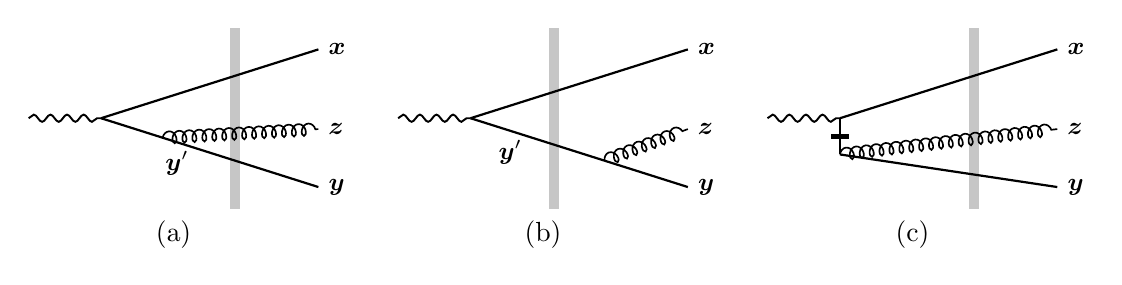
\begin{tikzpicture}[scale=0.92]
% (a)
\begin{scope}
\shock{0.55}
\draw[photon] (-2.3,0)--(-1.3,0);
\draw[quark] (-1.3,0)--(1.7,0.95) node[right]{\small $\x$};
\draw[quark] (-1.3,0)--(1.7,-0.95) node[right]{\small $\y$};
\draw[gluon] (-0.45,-0.27)--(1.7,-0.15) node[right]{\small $\z$};
\node at (-0.25,-0.62) {\small $\yp$};
\node at (-0.3,-1.6) {(a)};
\end{scope}
% (b)
\begin{scope}[xshift=5.1cm]
\shock{-0.15}
\draw[photon] (-2.3,0)--(-1.3,0);
\draw[quark] (-1.3,0)--(1.7,0.95) node[right]{\small $\x$};
\draw[quark] (-1.3,0)--(1.7,-0.95) node[right]{\small $\y$};
\draw[gluon] (0.55,-0.585)--(1.7,-0.15) node[right]{\small $\z$};
\node at (-0.75,-0.47) {\small $\yp$};
\node at (-0.3,-1.6) {(b)};
\end{scope}
% (c)
\begin{scope}[xshift=10.2cm]
\shock{0.55}
\draw[photon] (-2.3,0)--(-1.3,0);
\draw[quark] (-1.3,0)--(1.7,0.95) node[right]{\small $\x$};
\draw[quark] (-1.3,0)--(-1.3,-0.5);
\draw[line width=1.6pt] (-1.42,-0.25)--(-1.18,-0.25);
\draw[quark] (-1.3,-0.5)--(1.7,-0.95) node[right]{\small $\y$};
\draw[gluon] (-1.3,-0.5)--(1.7,-0.15) node[right]{\small $\z$};
\node at (-0.3,-1.6) {(c)};
\end{scope}
\end{tikzpicture}
\caption{Gluon emission by the antiquark. (a) The gluon is emitted before the collision with the
shock wave (grey band) and the three partons scatter. (b) The gluon is emitted after the collision and
only the quark--antiquark pair scatters, at the transverse positions $\x$ and $\yp$. (c) Instantaneous
graph: the photon decay and the gluon emission occur at the same light-cone time (the instantaneous
antiquark propagator is marked by a bar). The graphs in which the photon crosses the shock wave
before decaying are taken into account by the subtraction $\hat S\to\hat S-1$.}
\label{fig:qbar}
\end{figure}

\subsection{Gluon emission by the antiquark}
\label{sec:qbar}

\subsubsection{Emission before the collision}
\label{sec:before}

Inserting the matrix elements \eqref{eq:Hgamma2} and \eqref{eq:Hg}--\eqref{eq:Hg2} and the energy
denominators \eqref{eq:den1} and \eqref{eq:den3} in the first line of eq.~\eqref{eq:formal} with
$\hat S\to1$, we find
\begin{align}
\big|\gamma_T^i(Q,q^+,\qq)\big\rangle^{(a)}_{\qqg}=&-\frac{1}{(2\pi)^6}\int\dd^2\kt\,\dd^2\pt
\int_0^1\dd\zeta\int_0^{1-\zeta}\dd\xi\;
\frac{e\,e_f\,g\,q^+\,\zeta(1-\zeta)}{2\sqrt\xi\,\big(\kt^2+\ef^2\big)}
\nonumber\\
&\times\frac{\big[\varphi^{ij}_{\lambda_1\lambda}(\zeta)\,\kt^j+\mf\,\mu^i_{\lambda_1\lambda}\big]
\big[\tau^{mn}_{\lambda\lambda_2}(\xi,\eta)\,\pt^{\,n}+\xi\,\of\,\mu^m_{\lambda\lambda_2}\big]\,t^a_{\alpha\beta}}
{\zeta(1-\zeta)^2\big(\pt^{\,2}+\of^2\big)+\xi\eta\big(\kt^2+\ef^2\big)}
\nonumber\\
&\times\big|\bar q^\beta_{\lambda_2}(\eta q^+,\qq-\kk-\pp)\;g^a_m(\xi q^+,\pp)\;q^\alpha_{\lambda_1}(\zeta q^+,\kk)\big\rangle\,,
\label{eq:wf-mom}
\end{align}
where repeated helicity, polarisation and colour indices are summed over. The numerator is the product
of the two vertices in eq.~\eqref{eq:vertices} and contains four terms, which correspond to the four
helicity paths: no flip ($\varphi\,\tau$), flip at the gluon vertex ($\varphi\,\mu$), flip at the photon
vertex ($\mu\,\tau$), and double flip ($\mu\,\mu$).

To go to the transverse coordinate representation we write
\begin{equation}
\big|\bar q^\beta_{\lambda_2}(\qq-\kk-\pp)\,g^a_m(\pp)\,q^\alpha_{\lambda_1}(\kk)\big\rangle
=\int_{\x,\y,\z}e^{i\kk\cdot\x+i\pp\cdot\z+i(\qq-\kk-\pp)\cdot\y}\;
\big|\bar q^\beta_{\lambda_2}(\y)\,g^a_m(\z)\,q^\alpha_{\lambda_1}(\x)\big\rangle\,,
\end{equation}
and we express $\kk$ and $\pp$ in terms of $\kt$ and $\pt$. The phase becomes
\begin{equation}
e^{i\kk\cdot\x+i\pp\cdot\z+i(\qq-\kk-\pp)\cdot\y}=e^{i\w\cdot\qq}\;e^{i\R\cdot\kt}\;e^{-i\Y\cdot\pt}\,,
\label{eq:phase}
\end{equation}
where
\begin{equation}
\w=\zeta\x+(1-\zeta)\yp=\zeta\x+\eta\y+\xi\z\equiv\cc\,,\qquad
\yp\equiv\frac{\eta\y+\xi\z}{1-\zeta}\,,\qquad \R\equiv\x-\yp\,,\qquad\Y\equiv\y-\z\,.
\label{eq:coords}
\end{equation}
Here $\yp$ is the transverse position of the antiquark before the emission, which coincides with the
centre of energy of the final antiquark--gluon pair, $\cc$ is the centre of energy of the three-parton
system, which coincides with the position $\w$ of the photon, and $\R$ and $\Y$ are the transverse
separations of the daughter partons at the two vertices.

In the massless case the Fourier transform of eq.~\eqref{eq:wf-mom} is given by the well-known
formula~\cite{Beuf:2017bpd,Iancu:2022gpw}
\begin{equation}
\int\frac{\dd^2\kk}{2\pi}\frac{\dd^2\pp}{2\pi}\;
\frac{k^i\,p^j\;e^{i\kk\cdot\X+i\pp\cdot\bm{Z}}}{\big(\kk^2+\bar Q^2\big)\big[a(\kk^2+\bar Q^2)+\pp^2\big]}
=-\frac{X^iZ^j}{\bm{Z}^2}\;\frac{\bar Q\,K_1\big(\bar Q\sqrt{\X^2+a\bm{Z}^2}\big)}{\sqrt{\X^2+a\bm{Z}^2}}\,,
\label{eq:FT-massless}
\end{equation}
which involves a single modified Bessel function. With massive quarks, the two denominators of
eq.~\eqref{eq:wf-mom} contain two different scales, $\ef$ and $\of$, and each of the four helicity paths
has a different transform. We define four radial functions $\cG^{(\alpha\beta)}(\R,\Y)$, with
$\alpha,\beta\in\{0,1\}$ counting the powers of $\kt$ and $\pt$ in the numerator, by
\begin{align}
(1-\zeta)\int\frac{\dd^2\kt}{2\pi}\frac{\dd^2\pt}{2\pi}\;&
\frac{e^{i\kt\cdot\R}\,e^{-i\pt\cdot\Y}\;\big\{\kt^j\pt^{\,n},\;\kt^j,\;\pt^{\,n},\;1\big\}}
{\big(\kt^2+\ef^2\big)\Big[\zeta(1-\zeta)^2\big(\pt^{\,2}+\of^2\big)+\xi\eta\big(\kt^2+\ef^2\big)\Big]}
\nonumber\\
&=\Big\{R^jY^n\,\cG^{(11)},\;\;i\,R^j\,\cG^{(10)},\;\;-i\,Y^n\,\cG^{(01)},\;\;\cG^{(00)}\Big\}\,.
\label{eq:Gdef}
\end{align}
Using a Schwinger parametrisation of the two denominators and performing the Gaussian integrals (see
appendix~\ref{app:radial}), one of the two Schwinger integrals can be done in closed form and we obtain
\begin{equation}
\boxed{\;\cG^{(\alpha\beta)}(\R,\Y)=\frac{a^\beta}{2\zeta(1-\zeta)}\int_0^1\frac{\dd u}{u^{1+\beta}}
\left(\frac{A_u}{\Delta_u}\right)^{\frac{\alpha+\beta}{2}}K_{\alpha+\beta}\Big(\sqrt{A_u\,\Delta_u}\Big)\,,
\qquad\alpha,\beta\in\{0,1\}\,,\;}
\label{eq:Gab}
\end{equation}
with
\begin{equation}
A_u\equiv\ef^2+\frac{u\,\of^2}{a}=\zeta(1-\zeta)Q^2+\mf^2\left(1+\frac{u\,\zeta\,\xi}{\eta}\right)\,,\qquad
\Delta_u\equiv\R^2+\frac{a\,\Y^2}{u}\,,
\label{eq:ADelta}
\end{equation}
and $K_\nu$ the modified Bessel function of the second kind. Explicitly,
\begin{align}
\cG^{(11)}&=\frac{a}{2\zeta(1-\zeta)}\int_0^1\frac{\dd u}{u^2}\;\frac{A_u}{\Delta_u}\,
K_2\Big(\sqrt{A_u\Delta_u}\Big)\,,
\nonumber\\
\cG^{(10)}&=\frac{1}{2\zeta(1-\zeta)}\int_0^1\frac{\dd u}{u}\,\sqrt{\frac{A_u}{\Delta_u}}\;
K_1\Big(\sqrt{A_u\Delta_u}\Big)\,,
\nonumber\\
\cG^{(01)}&=\frac{a}{2\zeta(1-\zeta)}\int_0^1\frac{\dd u}{u^2}\,\sqrt{\frac{A_u}{\Delta_u}}\;
K_1\Big(\sqrt{A_u\Delta_u}\Big)\,,
\nonumber\\
\cG^{(00)}&=\frac{1}{2\zeta(1-\zeta)}\int_0^1\frac{\dd u}{u}\;K_0\Big(\sqrt{A_u\Delta_u}\Big)\,.
\label{eq:Gexplicit}
\end{align}
The integrals converge at $u\to0$ thanks to the exponential decay of the Bessel functions, since
$\Delta_u\to\infty$ there. The parameter $u$ has a simple interpretation: it is the fraction of the
total Schwinger ``time'' which is spent in the three-parton state. For $\mf=0$ one has $A_u=\bar
Q^2\equiv\zeta(1-\zeta)Q^2$, the $u$-integral in $\cG^{(11)}$ can be performed and
eq.~\eqref{eq:FT-massless} is recovered, see section~\ref{sec:massless}.

In terms of these functions, and after adding the Wilson lines for the three partons which cross the
shock wave and subtracting the no-scattering limit, the contribution of the graph in
figure~\ref{fig:qbar}(a) reads
\begin{align}
\big|\gamma_T^i(Q,q^+,\w)\big\rangle^{(a)}_{\qqg}=&-\frac{e\,e_f\,g\,q^+}{2(2\pi)^4}\int_{\x,\y,\z}
\int_0^1\dd\zeta\int_0^{1-\zeta}\dd\xi\;\frac{\zeta}{\sqrt\xi}\;\delta^{(2)}(\w-\cc)\;
\Psi^{im}_{\lambda_1\lambda_2}[\cG](\R,\Y)
\nonumber\\
&\times\Big[U^{ab}(\z)\,V(\x)\,t^b\,V^\dagger(\y)-t^a\Big]_{\alpha\beta}\;
\big|\bar q^\beta_{\lambda_2}(\eta q^+,\y)\;g^a_m(\xi q^+,\z)\;q^\alpha_{\lambda_1}(\zeta q^+,\x)\big\rangle\,,
\label{eq:wf-a}
\end{align}
where $V$ and $U$ are Wilson lines in the fundamental and in the adjoint representation,
\begin{equation}
V(\x)={\rm T}\exp\left\{ig\int\dd x^+\,t^a A^-_a(x^+,\x)\right\}\,,\qquad
U(\x)={\rm T}\exp\left\{ig\int\dd x^+\,T^a A^-_a(x^+,\x)\right\}\,,
\end{equation}
and where, for a generic set of four radial functions $F=\{F^{(11)},F^{(10)},F^{(01)},F^{(00)}\}$,
\begin{align}
\Psi^{im}_{\lambda_1\lambda_2}[F](\R,\Y)\equiv\sum_\lambda\Big[&
\varphi^{ij}_{\lambda_1\lambda}(\zeta)\,\tau^{mn}_{\lambda\lambda_2}(\xi,\eta)\,R^jY^n\,F^{(11)}
+i\,\xi\,\of\;\varphi^{ij}_{\lambda_1\lambda}(\zeta)\,\mu^m_{\lambda\lambda_2}\,R^j\,F^{(10)}
\nonumber\\
&-i\,\mf\;\mu^i_{\lambda_1\lambda}\,\tau^{mn}_{\lambda\lambda_2}(\xi,\eta)\,Y^n\,F^{(01)}
+\mf\,\xi\,\of\;\mu^i_{\lambda_1\lambda}\,\mu^m_{\lambda\lambda_2}\,F^{(00)}\Big]\,.
\label{eq:Psi}
\end{align}
The upper indices $i$ and $m$ are the polarisations of the photon and of the gluon. The four terms in
eq.~\eqref{eq:Psi} are the four helicity paths; the first one is the only one which survives when
$\mf\to0$.

The argument of the Bessel functions shows how the virtuality of the photon limits the transverse size
of the partonic fluctuation before the collision. In the massless case this size is the distance $\cD$
defined by
\begin{equation}
\cD^2(\x,\y,\z)\equiv\zeta(1-\zeta)\R^2+\frac{\xi\eta}{1-\zeta}\Y^2
=\zeta\eta(\x-\y)^2+\zeta\xi(\x-\z)^2+\eta\xi(\y-\z)^2\,,
\label{eq:D}
\end{equation}
with $Q\cD\lesssim1$. In the massive case one has $\sqrt{A_u\Delta_u}\geq\ef R$ for all $u$, with
$\ef>\mf$: the size of the quark--antiquark pair is limited by the Compton wavelength of the heavy
quark even in the photoproduction limit $Q^2\to0$, where all the functions \eqref{eq:Gexplicit} remain
finite.

\subsubsection{Emission after the collision}
\label{sec:after}

For the graph in figure~\ref{fig:qbar}(b) the only differences with respect to the previous case are
one energy denominator and the Wilson lines. According to eq.~\eqref{eq:formal}, the denominator
$E_{\qqg}-E_\gamma$ is replaced by $E_{\qqbar}-E_{\qqg}$, that is,
\begin{equation}
\frac{1}{\zeta(1-\zeta)^2\big(\pt^{\,2}+\of^2\big)+\xi\eta\big(\kt^2+\ef^2\big)}\;\longrightarrow\;
-\frac{1}{\zeta(1-\zeta)^2\big(\pt^{\,2}+\of^2\big)}\,.
\label{eq:replace}
\end{equation}
The two transverse integrations now factorise. Using
\begin{align}
\int\frac{\dd^2\kt}{2\pi}\;\frac{e^{i\kt\cdot\R}\,\{\kt^j,1\}}{\kt^2+\ef^2}
&=\left\{\frac{iR^j}{R}\,\ef K_1(\ef R)\,,\;K_0(\ef R)\right\}\,,
\nonumber\\
\int\frac{\dd^2\pt}{2\pi}\;\frac{e^{-i\pt\cdot\Y}\,\{\pt^{\,n},1\}}{\pt^{\,2}+\of^2}
&=\left\{-\frac{iY^n}{Y}\,\of K_1(\of Y)\,,\;K_0(\of Y)\right\}\,,
\label{eq:FT-fact}
\end{align}
with $R\equiv|\R|$ and $Y\equiv|\Y|$, we define the analogue of eq.~\eqref{eq:Gdef},
\begin{align}
(1-\zeta)\int\frac{\dd^2\kt}{2\pi}\frac{\dd^2\pt}{2\pi}\;&
\frac{e^{i\kt\cdot\R}\,e^{-i\pt\cdot\Y}\;\big\{\kt^j\pt^{\,n},\;\kt^j,\;\pt^{\,n},\;1\big\}}
{\big(\kt^2+\ef^2\big)\,\zeta(1-\zeta)^2\big(\pt^{\,2}+\of^2\big)}
\nonumber\\
&=\Big\{R^jY^n\,\cA^{(11)},\;\;i\,R^j\,\cA^{(10)},\;\;-i\,Y^n\,\cA^{(01)},\;\;\cA^{(00)}\Big\}\,,
\label{eq:Adef}
\end{align}
with the factorised functions
\begin{align}
\cA^{(11)}&=\frac{\ef K_1(\ef R)}{\zeta(1-\zeta)\,R}\;\frac{\of K_1(\of Y)}{Y}\,,
&\cA^{(10)}&=\frac{\ef K_1(\ef R)}{\zeta(1-\zeta)\,R}\;K_0(\of Y)\,,
\nonumber\\
\cA^{(01)}&=\frac{K_0(\ef R)}{\zeta(1-\zeta)}\;\frac{\of K_1(\of Y)}{Y}\,,
&\cA^{(00)}&=\frac{K_0(\ef R)}{\zeta(1-\zeta)}\;K_0(\of Y)\,.
\label{eq:Aexplicit}
\end{align}
Each of them is the product of a leading-order photon wave function, $\ef K_1(\ef R)$ or $K_0(\ef R)$,
and of an emission kernel off the massive antiquark, $\of K_1(\of Y)/Y$ or $K_0(\of Y)$. The massless
emission kernel $Y^n/Y^2$, which has a power-like tail at large $Y$, is thus replaced by
$Y^n\of K_1(\of Y)/Y$, which decays exponentially for $Y\gtrsim1/\of$: this is the dead-cone
effect in transverse coordinate space.

In this graph only the intermediate quark--antiquark pair, at transverse positions $\x$ and $\yp$,
scatters, and the colour matrix of the emission vertex stands to the right of the Wilson lines. We get
\begin{align}
\big|\gamma_T^i(Q,q^+,\w)\big\rangle^{(b)}_{\qqg}=&+\frac{e\,e_f\,g\,q^+}{2(2\pi)^4}\int_{\x,\y,\z}
\int_0^1\dd\zeta\int_0^{1-\zeta}\dd\xi\;\frac{\zeta}{\sqrt\xi}\;\delta^{(2)}(\w-\cc)\;
\Psi^{im}_{\lambda_1\lambda_2}[\cA](\R,\Y)
\nonumber\\
&\times\Big[V(\x)\,V^\dagger(\yp)\,t^a-t^a\Big]_{\alpha\beta}\;
\big|\bar q^\beta_{\lambda_2}(\eta q^+,\y)\;g^a_m(\xi q^+,\z)\;q^\alpha_{\lambda_1}(\zeta q^+,\x)\big\rangle\,.
\label{eq:wf-b}
\end{align}
The Wilson-line structure of eq.~\eqref{eq:wf-b} is obtained from that of eq.~\eqref{eq:wf-a} by
letting $\y,\z\to\yp$, because $U^{ab}(\yp)V(\x)t^bV^\dagger(\yp)=V(\x)V^\dagger(\yp)t^a$. In
contrast with the massless case, however, the radial functions $\cA^{(\alpha\beta)}$ are not simply the
coincidence limit of the functions $\cG^{(\alpha\beta)}$; they only share their short-distance
singularities, see eq.~\eqref{eq:UV} below.

\subsubsection{Instantaneous contribution}
\label{sec:inst}

For the graph in figure~\ref{fig:qbar}(c) there is a single energy denominator, $E_{\qqg}-E_\gamma$, and
the matrix element \eqref{eq:Hinst}. In momentum space and without scattering,
\begin{align}
\big|\gamma_T^i\big\rangle^{({\rm inst})}_{\qqg}=&\frac{1}{(2\pi)^6}\int\dd^2\kt\,\dd^2\pt
\int_0^1\dd\zeta\int_0^{1-\zeta}\dd\xi\;\frac{e\,e_f\,g\,q^+\,\zeta}{2\sqrt\xi}\;
\frac{\xi\eta\;\big(\delta^{im}+2i\ee^{im}\lambda_1\big)\,\delta_{\lambda_1\lambda_2}\,t^a_{\alpha\beta}}
{\zeta(1-\zeta)^2\big(\pt^{\,2}+\of^2\big)+\xi\eta\big(\kt^2+\ef^2\big)}
\nonumber\\
&\times\big|\bar q^\beta_{\lambda_2}(\eta q^+,\qq-\kk-\pp)\;g^a_m(\xi q^+,\pp)\;q^\alpha_{\lambda_1}(\zeta q^+,\kk)\big\rangle\,.
\end{align}
The denominator is a single quadratic form in $(\kt,\pt)$, whose constant term is given by
eq.~\eqref{eq:Ef}. Its Fourier transform is therefore the massless one with $Q\to\Ef$:
\begin{equation}
(1-\zeta)\int\frac{\dd^2\kt}{2\pi}\frac{\dd^2\pt}{2\pi}\;
\frac{e^{i\kt\cdot\R}\,e^{-i\pt\cdot\Y}}{\zeta(1-\zeta)^2\big(\pt^{\,2}+\of^2\big)+\xi\eta\big(\kt^2+\ef^2\big)}
=\frac{\Ef\,K_1(\Ef\,\cD)}{\cD}\equiv\cG_E\,,
\label{eq:GE}
\end{equation}
with $\cD$ given by eq.~\eqref{eq:D}. The three partons scatter, so that the Wilson-line structure is the
same as in eq.~\eqref{eq:wf-a}:
\begin{align}
\big|\gamma_T^i(Q,q^+,\w)\big\rangle^{({\rm inst})}_{\qqg}=&\frac{e\,e_f\,g\,q^+}{2(2\pi)^4}\int_{\x,\y,\z}
\int_0^1\dd\zeta\int_0^{1-\zeta}\dd\xi\;\frac{\zeta\,\eta\,\sqrt\xi}{1-\zeta}\;\delta^{(2)}(\w-\cc)
\nonumber\\
&\times\big(\delta^{im}+2i\ee^{im}\lambda_1\big)\,\delta_{\lambda_1\lambda_2}\;\cG_E\;
\Big[U^{ab}(\z)\,V(\x)\,t^b\,V^\dagger(\y)-t^a\Big]_{\alpha\beta}
\nonumber\\
&\times\big|\bar q^\beta_{\lambda_2}(\eta q^+,\y)\;g^a_m(\xi q^+,\z)\;q^\alpha_{\lambda_1}(\zeta q^+,\x)\big\rangle\,.
\label{eq:wf-inst}
\end{align}
There is no instantaneous counterpart of the graph in figure~\ref{fig:qbar}(b), since an instantaneous
propagator cannot cross the shock wave.

\subsubsection{Summary: effective vertices}
\label{sec:eff}

The three contributions \eqref{eq:wf-a}, \eqref{eq:wf-b} and \eqref{eq:wf-inst} can be combined in a
single expression,
\begin{align}
\big|\gamma_T^i(Q,q^+,\w)\big\rangle^{(\bar q)}_{\qqg}=&-\frac{e\,e_f\,g\,q^+}{2(2\pi)^4}\int_{\x,\y,\z}
\int_0^1\dd\zeta\int_0^{1-\zeta}\dd\xi\;\frac{\zeta}{\sqrt\xi}\;\delta^{(2)}(\w-\cc)
\nonumber\\
&\times\bigg\{\cM^{im}_{1\,\lambda_1\lambda_2}\,\Big[U^{ab}(\z)\,V(\x)\,t^b\,V^\dagger(\y)-t^a\Big]_{\alpha\beta}
\nonumber\\
&\qquad\;-\cM^{im}_{2\,\lambda_1\lambda_2}\,\Big[V(\x)\,V^\dagger(\yp)\,t^a-t^a\Big]_{\alpha\beta}\bigg\}
\nonumber\\
&\times\big|\bar q^\beta_{\lambda_2}(\eta q^+,\y)\;g^a_m(\xi q^+,\z)\;q^\alpha_{\lambda_1}(\zeta q^+,\x)\big\rangle\,,
\label{eq:state-qbar}
\end{align}
with the effective vertices
\begin{align}
\cM^{im}_{1\,\lambda_1\lambda_2}(\x,\y,\z)&=\Psi^{im}_{\lambda_1\lambda_2}[\cG](\R,\Y)
-\delta_{\lambda_1\lambda_2}\,\frac{\xi\,\eta}{1-\zeta}\,\big(\delta^{im}+2i\ee^{im}\lambda_1\big)\,\cG_E\,,
\nonumber\\
\cM^{im}_{2\,\lambda_1\lambda_2}(\x,\y,\z)&=\Psi^{im}_{\lambda_1\lambda_2}[\cA](\R,\Y)\,.
\label{eq:M}
\end{align}
The superscript $(\bar q)$ recalls that the gluon is emitted by the antiquark.

A comment is in order about the ultraviolet behaviour at $\Y\to0$, i.e.\ when the gluon is close to its
emitter. Each of the two terms of eq.~\eqref{eq:state-qbar} is singular in this limit, but their
Wilson-line structures become identical and the singularities cancel in the difference, provided that
the radial functions have the same singular behaviour. This is indeed the case: we find
\begin{align}
&\Y^2\,\cG^{(11)}\to\frac{\ef K_1(\ef R)}{\zeta(1-\zeta)R}\,,\qquad
\Y^2\,\cG^{(01)}\to\frac{K_0(\ef R)}{\zeta(1-\zeta)}\,,\qquad
\nonumber\\
&\cG^{(10)}-\cA^{(10)}\to{\rm finite}\,,\qquad\cG^{(00)}-\cA^{(00)}\to{\rm finite}\,,
\qquad\text{for }\Y\to0\,,
\label{eq:UV}
\end{align}
which are the limits of $\Y^2\cA^{(11)}$ and $\Y^2\cA^{(01)}$; the functions $\cG^{(10)}$ and
$\cG^{(00)}$ are only logarithmically singular. The instantaneous term is regular at $\Y\to0$.

\begin{figure}[t]
\centering
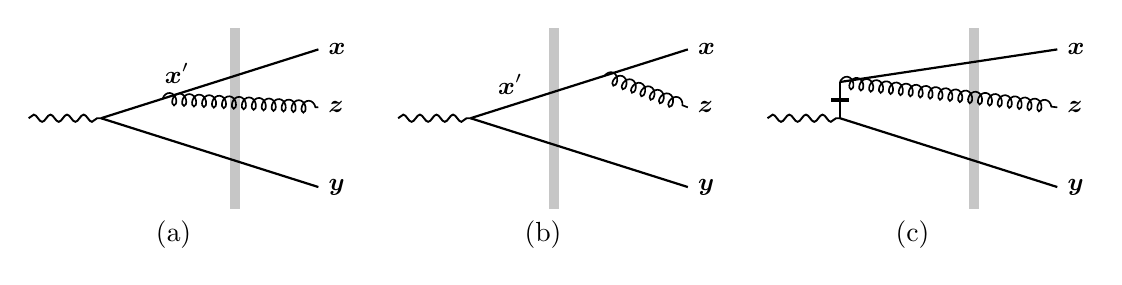
\begin{tikzpicture}[scale=0.92]
\begin{scope}
\shock{0.55}
\draw[photon] (-2.3,0)--(-1.3,0);
\draw[quark] (-1.3,0)--(1.7,0.95) node[right]{\small $\x$};
\draw[quark] (-1.3,0)--(1.7,-0.95) node[right]{\small $\y$};
\draw[gluon] (-0.45,0.27)--(1.7,0.15) node[right]{\small $\z$};
\node at (-0.25,0.62) {\small $\xp$};
\node at (-0.3,-1.6) {(a)};
\end{scope}
\begin{scope}[xshift=5.1cm]
\shock{-0.15}
\draw[photon] (-2.3,0)--(-1.3,0);
\draw[quark] (-1.3,0)--(1.7,0.95) node[right]{\small $\x$};
\draw[quark] (-1.3,0)--(1.7,-0.95) node[right]{\small $\y$};
\draw[gluon] (0.55,0.585)--(1.7,0.15) node[right]{\small $\z$};
\node at (-0.75,0.47) {\small $\xp$};
\node at (-0.3,-1.6) {(b)};
\end{scope}
\begin{scope}[xshift=10.2cm]
\shock{0.55}
\draw[photon] (-2.3,0)--(-1.3,0);
\draw[quark] (-1.3,0)--(1.7,-0.95) node[right]{\small $\y$};
\draw[quark] (-1.3,0)--(-1.3,0.5);
\draw[line width=1.6pt] (-1.42,0.25)--(-1.18,0.25);
\draw[quark] (-1.3,0.5)--(1.7,0.95) node[right]{\small $\x$};
\draw[gluon] (-1.3,0.5)--(1.7,0.15) node[right]{\small $\z$};
\node at (-0.3,-1.6) {(c)};
\end{scope}
\end{tikzpicture}
\caption{Gluon emission by the quark: (a) before the collision, (b) after the collision, where the
quark--antiquark pair scatters at the transverse positions $\xp$ and $\y$, and (c) instantaneous
graph.}
\label{fig:q}
\end{figure}

\subsection{Gluon emission by the quark}
\label{sec:q}

The contribution of the graphs in figure~\ref{fig:q} is obtained from eq.~\eqref{eq:state-qbar} by
exchanging the roles of the quark and of the antiquark while keeping the final state fixed: one
exchanges $\zeta\leftrightarrow\eta$, $\x\leftrightarrow\y$, $\lambda_1\leftrightarrow\lambda_2$ and
$\alpha\leftrightarrow\beta$, takes the complex conjugate of the integrand, and changes the overall
sign~\cite{Iancu:2022gpw}. The transverse coordinates transform as
\begin{equation}
\yp\to\xp\equiv\frac{\zeta\x+\xi\z}{\zeta+\xi}\,,\qquad
\R=\x-\yp\;\to\;\y-\xp\equiv-\Rt\,,\qquad\Y=\y-\z\;\to\;\x-\z\equiv\X\,,
\label{eq:coords-q}
\end{equation}
where $\xp$ is the position of the quark before the emission, $\Rt=\xp-\y$ is the size of the pair
produced by the photon and $\X$ the separation between the gluon and the final quark. The
helicity-conserving vertices transform as
\begin{align}
\varphi^{ij}_{\lambda_1\lambda}(\zeta)&\to\varphi^{ij\,*}_{\lambda_2\lambda}(\eta)
=-\varphi^{ij}_{\lambda\lambda_2}(\zeta+\xi)\,,\qquad
\tau^{mn}_{\lambda\lambda_2}(\xi,\eta)\to\tau^{mn\,*}_{\lambda\lambda_1}(\xi,\zeta)
=\tau^{nm}_{\lambda_1\lambda}(\xi,\zeta)\,,
\nonumber\\
\tau^{nm}_{\lambda_1\lambda}(\xi,\zeta)&=\delta_{\lambda_1\lambda}\big[(2\zeta+\xi)\,\delta^{nm}
+2i\,\xi\,\ee^{nm}\lambda\big]\,,
\label{eq:vert-q}
\end{align}
while the helicity-flip vertices become $\mf\,\mu^i_{\lambda\lambda_2}$ at the photon vertex and
$\xi\,\oft\,\mu^m_{\lambda_1\lambda}$ at the gluon vertex. The scales transform as
$\ef\to\eft$, $\of\to\oft$ and $a\to\tilde a$, cf.\ eq.~\eqref{eq:notation-q}, whereas $\cD$, $\Ef$ and
hence $\cG_E$ are invariant. The radial functions become
\begin{equation}
\tG^{(\alpha\beta)}(\Rt,\X)=\frac{\tilde a^{\,\beta}}{2\eta(1-\eta)}\int_0^1\frac{\dd u}{u^{1+\beta}}
\left(\frac{\tilde A_u}{\tilde\Delta_u}\right)^{\frac{\alpha+\beta}{2}}
K_{\alpha+\beta}\Big(\sqrt{\tilde A_u\,\tilde\Delta_u}\Big)\,,
\label{eq:Gtab}
\end{equation}
with
\begin{equation}
\tilde A_u=\eta(1-\eta)Q^2+\mf^2\left(1+\frac{u\,\eta\,\xi}{\zeta}\right)\,,\qquad
\tilde\Delta_u=\Rt^{\,2}+\frac{\tilde a\,\X^2}{u}\,,
\end{equation}
and
\begin{align}
\tA^{(11)}&=\frac{\eft K_1(\eft\tilde R)}{\eta(1-\eta)\,\tilde R}\;\frac{\oft K_1(\oft X)}{X}\,,
&\tA^{(10)}&=\frac{\eft K_1(\eft\tilde R)}{\eta(1-\eta)\,\tilde R}\;K_0(\oft X)\,,
\nonumber\\
\tA^{(01)}&=\frac{K_0(\eft\tilde R)}{\eta(1-\eta)}\;\frac{\oft K_1(\oft X)}{X}\,,
&\tA^{(00)}&=\frac{K_0(\eft\tilde R)}{\eta(1-\eta)}\;K_0(\oft X)\,.
\label{eq:Atexplicit}
\end{align}
Performing these transformations in eq.~\eqref{eq:state-qbar}, we find
\begin{align}
\big|\gamma_T^i(Q,q^+,\w)\big\rangle^{(q)}_{\qqg}=&+\frac{e\,e_f\,g\,q^+}{2(2\pi)^4}\int_{\x,\y,\z}
\int_0^1\dd\zeta\int_0^{1-\zeta}\dd\xi\;\frac{\eta}{\sqrt\xi}\;\delta^{(2)}(\w-\cc)
\nonumber\\
&\times\bigg\{\tM^{im}_{1\,\lambda_1\lambda_2}\,\Big[U^{ab}(\z)\,V(\x)\,t^b\,V^\dagger(\y)-t^a\Big]_{\alpha\beta}
\nonumber\\
&\qquad\;-\tM^{im}_{2\,\lambda_1\lambda_2}\,\Big[t^a\,V(\xp)\,V^\dagger(\y)-t^a\Big]_{\alpha\beta}\bigg\}
\nonumber\\
&\times\big|\bar q^\beta_{\lambda_2}(\eta q^+,\y)\;g^a_m(\xi q^+,\z)\;q^\alpha_{\lambda_1}(\zeta q^+,\x)\big\rangle\,,
\label{eq:state-q}
\end{align}
with
\begin{align}
\tM^{im}_{1\,\lambda_1\lambda_2}(\x,\y,\z)&=\tPsi^{im}_{\lambda_1\lambda_2}[\tG](\Rt,\X)
-\delta_{\lambda_1\lambda_2}\,\frac{\zeta\,\xi}{\zeta+\xi}\,\big(\delta^{im}-2i\ee^{im}\lambda_1\big)\,\cG_E\,,
\nonumber\\
\tM^{im}_{2\,\lambda_1\lambda_2}(\x,\y,\z)&=\tPsi^{im}_{\lambda_1\lambda_2}[\tA](\Rt,\X)\,,
\label{eq:Mt}
\end{align}
and
\begin{align}
\tPsi^{im}_{\lambda_1\lambda_2}[\tF](\Rt,\X)\equiv\sum_\lambda\Big[&
\tau^{nm}_{\lambda_1\lambda}(\xi,\zeta)\,\varphi^{ij}_{\lambda\lambda_2}(\zeta+\xi)\,\tilde R^jX^n\,\tF^{(11)}
+i\,\xi\,\oft\;\mu^m_{\lambda_1\lambda}\,\varphi^{ij}_{\lambda\lambda_2}(\zeta+\xi)\,\tilde R^j\,\tF^{(10)}
\nonumber\\
&-i\,\mf\;\tau^{nm}_{\lambda_1\lambda}(\xi,\zeta)\,\mu^i_{\lambda\lambda_2}\,X^n\,\tF^{(01)}
+\mf\,\xi\,\oft\;\mu^m_{\lambda_1\lambda}\,\mu^i_{\lambda\lambda_2}\,\tF^{(00)}\Big]\,.
\label{eq:Psit}
\end{align}
As in the massless case, the Wilson-line structure of the graphs in which the gluon is emitted before
the collision is the same for the two emitters, whereas for an emission after the collision the colour
matrix now stands to the left of the Wilson lines; the latter structure is again obtained from the
former by letting $\x,\z\to\xp$, because $U^{ab}(\xp)V(\xp)t^b=t^aV(\xp)$. The relative sign and the
relative normalisation of eqs.~\eqref{eq:state-qbar} and \eqref{eq:state-q}, which control the
interference terms in the cross-section, have been checked against the complete Feynman amplitude
(appendix~\ref{app:checks}).

The complete $\qqg$ component of the outgoing state of the transverse photon is the sum
\begin{equation}
\big|\gamma_T^i(Q,q^+,\w)\big\rangle_{\qqg}=\big|\gamma_T^i(Q,q^+,\w)\big\rangle^{(\bar q)}_{\qqg}
+\big|\gamma_T^i(Q,q^+,\w)\big\rangle^{(q)}_{\qqg}\,.
\label{eq:state}
\end{equation}

\section{The trijet cross-section}
\label{sec:xs}

We now insert the outgoing state \eqref{eq:state} into eq.~\eqref{eq:xsdef}. The number-density
operators are expressed in the transverse coordinate representation,
\begin{equation}
N_q(k^+,\kk)=\frac{1}{(2\pi)^3}\int_{\x,\bx}e^{-i\kk\cdot(\x-\bx)}\;
b^{\alpha\dagger}_\lambda(k^+,\bx)\,b^{\alpha}_\lambda(k^+,\x)\,,
\end{equation}
and similarly for the antiquark and the gluon, and the Fock-space operators are contracted with those
of the state. The integrations over $\w$ and $\bar\w$ remove the $\delta$-functions which identify the
photon position with the centre of energy $\cc$. The cross-section is the sum of three terms: the
direct contributions of the antiquark and of the quark, in which the gluon is emitted by the same
fermion in the direct amplitude (DA) and in the complex-conjugate amplitude (CCA), and the
interference contribution,
\begin{equation}
\frac{\dd\sigma^{\gT A\to\qqg+X}}{\dd^3k_1\,\dd^3k_2\,\dd^3k_3}
=\frac{\dd\sigma^{(\bar q\bar q)}}{\dd^3k_1\,\dd^3k_2\,\dd^3k_3}
+\frac{\dd\sigma^{(qq)}}{\dd^3k_1\,\dd^3k_2\,\dd^3k_3}
+\frac{\dd\sigma^{(q\bar q)}}{\dd^3k_1\,\dd^3k_2\,\dd^3k_3}\,.
\label{eq:xs-sum}
\end{equation}
The longitudinal fractions are fixed by the final state, $\zeta=k_1^+/q^+$, $\xi=k_3^+/q^+$ and
$\eta=k_2^+/q^+=1-\zeta-\xi$, and are therefore the same in the DA and in the CCA. Coordinates and
functions with a bar refer to the CCA: for instance $\bR=\bx-\byp$, $\bY=\by-\bz$ and
$\bar F^{(\alpha\beta)}\equiv F^{(\alpha\beta)}(\bR,\bY)$. Since each of the amplitudes
\eqref{eq:state-qbar} and \eqref{eq:state-q} is the difference of two terms, each of the three
contributions in eq.~\eqref{eq:xs-sum} contains four terms.

\subsection{Colour structure}
\label{sec:colour}

The average over the colour fields of the target generates the $S$-matrices of colourless systems made
of up to six partons. For the terms in which the three partons scatter both in the DA and in the CCA we
need
\begin{align}
\cS_{\qqg\,\qqg}(\x,\y,\z;\bx,\by,\bz)&\equiv\frac{1}{\CF\Nc}\Big\langle\big[U^\dagger(\bz)U(\z)\big]^{ab}\;
\tr\big[V(\by)\,t^a\,V^\dagger(\bx)\,V(\x)\,t^b\,V^\dagger(\y)\big]\Big\rangle\,,
\nonumber\\
\cS_{\qqg}(\x,\y,\z)&\equiv\frac{1}{\CF\Nc}\Big\langle U^{ab}(\z)\;
\tr\big[V(\x)\,t^b\,V^\dagger(\y)\,t^a\big]\Big\rangle\,,
\label{eq:S6}
\end{align}
where the brackets denote the CGC average. The trace of the product of the Wilson-line structure of
eq.~\eqref{eq:wf-a} with its complex conjugate is then $\CF\Nc\,\cW$, with
\begin{equation}
\cW(\x,\y,\z;\bx,\by,\bz)\equiv\cS_{\qqg\,\qqg}(\x,\y,\z;\bx,\by,\bz)-\cS_{\qqg}(\x,\y,\z)
-\cS^\dagger_{\qqg}(\bx,\by,\bz)+1\,.
\label{eq:W}
\end{equation}
These expressions hold for any $\Nc$. Since the Wilson-line structures for an emission after the
collision are the coincidence limits of the one in eq.~\eqref{eq:wf-a}, namely $\y,\z\to\yp$ for the
antiquark and $\x,\z\to\xp$ for the quark, all the colour structures that we need are obtained from
eq.~\eqref{eq:W} by taking the corresponding limits, in the DA and/or in the CCA.

At large $\Nc$ the adjoint Wilson line is the product of a fundamental and an anti-fundamental one,
and eq.~\eqref{eq:S6} reduces to products of dipoles and quadrupoles,
\begin{align}
S(\x,\y)&\equiv\frac{1}{\Nc}\Big\langle\tr\big[V(\x)V^\dagger(\y)\big]\Big\rangle\,,
\nonumber\\
\cQ(\x_1,\x_2,\x_3,\x_4)&\equiv\frac{1}{\Nc}\Big\langle\tr\big[V(\x_1)V^\dagger(\x_2)V(\x_3)V^\dagger(\x_4)\big]\Big\rangle\,,
\end{align}
namely $\cS_{\qqg\,\qqg}\simeq\cQ(\x,\z,\bz,\bx)\,\cQ(\z,\y,\by,\bz)$ and
$\cS_{\qqg}\simeq S(\x,\z)\,S(\z,\y)$~\cite{Iancu:2022gpw}. Hence
\begin{equation}
\cW(\x,\y,\z;\bx,\by,\bz)\simeq\cQ(\x,\z,\bz,\bx)\,\cQ(\z,\y,\by,\bz)-S(\x,\z)\,S(\z,\y)
-S(\bz,\bx)\,S(\by,\bz)+1\,.
\label{eq:W-largeN}
\end{equation}
The coincidence limits which are relevant for the emission by the antiquark are
\begin{align}
\cW(\x,\yp,\yp;\bx,\by,\bz)&\simeq\cQ(\x,\yp,\bz,\bx)\,S(\by,\bz)-S(\x,\yp)-S(\bz,\bx)\,S(\by,\bz)+1\,,
\nonumber\\
\cW(\x,\y,\z;\bx,\byp,\byp)&\simeq\cQ(\x,\z,\byp,\bx)\,S(\z,\y)-S(\x,\z)\,S(\z,\y)-S(\byp,\bx)+1\,,
\nonumber\\
\cW(\x,\yp,\yp;\bx,\byp,\byp)&\simeq\cQ(\x,\yp,\byp,\bx)-S(\x,\yp)-S(\byp,\bx)+1\,,
\label{eq:W-qbar}
\end{align}
those for the emission by the quark are
\begin{align}
\cW(\xp,\y,\xp;\bx,\by,\bz)&\simeq S(\bz,\bx)\,\cQ(\xp,\y,\by,\bz)-S(\xp,\y)-S(\bz,\bx)\,S(\by,\bz)+1\,,
\nonumber\\
\cW(\x,\y,\z;\bxp,\by,\bxp)&\simeq S(\x,\z)\,\cQ(\z,\y,\by,\bxp)-S(\x,\z)\,S(\z,\y)-S(\by,\bxp)+1\,,
\nonumber\\
\cW(\xp,\y,\xp;\bxp,\by,\bxp)&\simeq\cQ(\xp,\y,\by,\bxp)-S(\xp,\y)-S(\by,\bxp)+1\,,
\label{eq:W-q}
\end{align}
and the interference terms involve in addition
\begin{align}
\cW(\xp,\y,\xp;\bx,\byp,\byp)&\simeq S(\byp,\bx)\,S(\xp,\y)-S(\xp,\y)-S(\byp,\bx)+1
\nonumber\\
&=\big[S(\xp,\y)-1\big]\big[S(\byp,\bx)-1\big]\,.
\label{eq:W-int}
\end{align}
The last lines of eqs.~\eqref{eq:W-qbar} and \eqref{eq:W-q} have the same structure as the colour
factor of the leading-order dijet cross-section,
\begin{equation}
\cW_{\rm LO}(\x,\y;\bx,\by)\equiv\cQ(\x,\y,\by,\bx)-S(\x,\y)-S(\by,\bx)+1\,,
\label{eq:WLO}
\end{equation}
as expected for the graphs in which the gluon is emitted in the final state on both sides of the cut.

The dipole $S$-matrix can be taken from a solution of the BK equation or from a model. The quadrupole
is in general an independent correlator, but in the Gaussian approximation and at large
$\Nc$~\cite{Dominguez:2011wm,Iancu:2011ns,Iancu:2011nj} it can be expressed in terms of the dipole,
\begin{align}
\cQ(\x_1,\x_2,\x_3,\x_4)\simeq{}& S(\x_1,\x_2)\,S(\x_3,\x_4)
\nonumber\\
&-\frac{F(\x_1,\x_2;\x_3,\x_4)}{F(\x_1,\x_3;\x_2,\x_4)}\,
\Big[S(\x_1,\x_2)\,S(\x_3,\x_4)-S(\x_1,\x_4)\,S(\x_3,\x_2)\Big]\,,
\label{eq:Gauss}
\end{align}
with
\begin{equation}
F(\x_1,\x_2;\x_3,\x_4)\equiv\ln\frac{S(\x_1,\x_3)\,S(\x_2,\x_4)}{S(\x_1,\x_4)\,S(\x_2,\x_3)}\,.
\label{eq:F}
\end{equation}
Equation~\eqref{eq:Gauss} has the correct coincidence limits, $\cQ(\x_1,\x_2,\x_2,\x_4)=S(\x_1,\x_4)$ and
$\cQ(\x_1,\x_2,\x_3,\x_1)=S(\x_3,\x_2)$. With eqs.~\eqref{eq:W-largeN}--\eqref{eq:Gauss} the whole trijet
cross-section is expressed in terms of the dipole $S$-matrix alone.

\subsection{Direct contribution of the antiquark}
\label{sec:xs-qbar}

Using eq.~\eqref{eq:state-qbar} and $e^2g^2=(4\pi)^2\aem\as$, we find
\begin{align}
\frac{\dd\sigma^{(\bar q\bar q)}}{\dd^3k_1\,\dd^3k_2\,\dd^3k_3}=&\;
\frac{\aem\,\as\,\CF\Nc}{2(2\pi)^{10}}\;\frac{\zeta^2}{\xi\,(q^+)^2}\;
\delta\big(q^+-k_1^+-k_2^+-k_3^+\big)\sum_fe_f^2
\nonumber\\
&\times\int_{\x,\y,\z,\bx,\by,\bz}e^{-i\kk_1\cdot(\x-\bx)-i\kk_2\cdot(\y-\by)-i\kk_3\cdot(\z-\bz)}\;
\Big[\cH[\cG;\bar\cG]\;\cW(\x,\y,\z;\bx,\by,\bz)
\nonumber\\
&\qquad-\cH[\cA;\bar\cG]\;\cW(\x,\yp,\yp;\bx,\by,\bz)
-\cH[\cG;\bar\cA]\;\cW(\x,\y,\z;\bx,\byp,\byp)
\nonumber\\
&\qquad+\cH[\cA;\bar\cA]\;\cW(\x,\yp,\yp;\bx,\byp,\byp)\Big]\,.
\label{eq:xs-qbar}
\end{align}
The quark mass depends on the flavour, so the sum over flavours acts on the whole integrand. The
function $\cH$ is the sum over the helicities of the quark and the antiquark and over the polarisations
of the photon and of the gluon of the product of the effective vertices,
\begin{equation}
\cH[F;\bar F]\equiv\sum_{\lambda_1,\lambda_2}\sum_{l,r}\cM^{lr}_{\lambda_1\lambda_2}[F](\x,\y,\z)\;
\cM^{lr\,*}_{\lambda_1\lambda_2}[\bar F](\bx,\by,\bz)\,,
\label{eq:Hdef}
\end{equation}
where $F$ stands for either $\cG$ or $\cA$, with $\cM[\cG]\equiv\cM_1$ and $\cM[\cA]\equiv\cM_2$ of
eq.~\eqref{eq:M}. To treat the two cases on the same footing we associate to each set a fifth function
$F_E$, which multiplies the instantaneous term: $F_E=\cG_E$ for $F=\cG$ and $F_E=0$ for $F=\cA$. We
find $\cH[F;\bar F]=\cH_{\rm reg\times reg}+\cH_{\rm reg\times inst}+\cH_{\rm inst\times inst}$, where the
three terms are the following functionals of $F$ and $\bar F$:
\begin{subequations}
\label{eq:H-direct}
\begin{align}
\cH_{\rm reg\times reg}={}&\Big\{8\big[\zeta^2+(1-\zeta)^2\big]\big[\eta^2+(1-\zeta)^2\big]\,
(\R\cdot\bR)(\Y\cdot\bY)
\nonumber\\
&\quad-8\,\xi\,(2\zeta-1)\big(2(1-\zeta)-\xi\big)\,(\R\times\bR)(\Y\times\bY)\Big\}\,F^{(11)}\bar F^{(11)}
\nonumber\\
&+8\,\mf^2\big[\eta^2+(1-\zeta)^2\big]\,(\Y\cdot\bY)\,F^{(01)}\bar F^{(01)}
+8\,\mf^2\,\xi^2\of^2\,F^{(00)}\bar F^{(00)}
\nonumber\\
&+8\,\xi^2\of^2\big[\zeta^2+(1-\zeta)^2\big]\,(\R\cdot\bR)\,F^{(10)}\bar F^{(10)}
\nonumber\\
&-8\,\zeta\,\eta\,\mf\,\xi\,\of\Big[(\R\cdot\Y)\,F^{(11)}\bar F^{(00)}+(\bR\cdot\bY)\,F^{(00)}\bar F^{(11)}
\nonumber\\
&\hspace{2.6cm}+(\R\cdot\bY)\,F^{(10)}\bar F^{(01)}+(\Y\cdot\bR)\,F^{(01)}\bar F^{(10)}\Big]\,,
\label{eq:Hrr}\\[1mm]
\cH_{\rm reg\times inst}={}&-\frac{8\,\zeta\,\xi\,\eta^2}{1-\zeta}\,
\Big[(\R\cdot\Y)\,F^{(11)}\bar F_E+(\bR\cdot\bY)\,F_E\,\bar F^{(11)}\Big]
\nonumber\\
&+\frac{8\,\xi^2\,\eta\,\mf\,\of}{1-\zeta}\,\Big[F^{(00)}\bar F_E+F_E\,\bar F^{(00)}\Big]\,,
\label{eq:Hri}\\[1mm]
\cH_{\rm inst\times inst}={}&8\left[\frac{\xi\,\eta}{1-\zeta}\right]^2F_E\,\bar F_E\,,
\label{eq:Hii}
\end{align}
\end{subequations}
where $\bm{A}\times\bm{B}\equiv\ee^{ij}A^iB^j$. The first two lines of eq.~\eqref{eq:Hrr}, together
with the first line of eq.~\eqref{eq:Hri} and with eq.~\eqref{eq:Hii}, are the massless structures. The
mass generates (i) three ``diagonal'' terms, in which the same helicity path is followed in the DA and
in the CCA, with weights given by the squares of the photon splitting factor
$\zeta^2+(1-\zeta)^2$ or of the gluon splitting factor $\eta^2+(1-\zeta)^2$ and by the squares of the
flip vertices $\mf$ and $\xi\of$; (ii) four terms in which two different paths interfere, namely the
no-flip path with the double-flip path and the two single-flip paths with each other, all with the
common weight $-8\zeta\eta\,\mf\,\xi\of$; and (iii) the interference of the double-flip path with the
instantaneous term. Paths with a different total number of flips do not interfere, since they lead to
different final helicities.

\subsection{Direct contribution of the quark}
\label{sec:xs-q}

Similarly, from eq.~\eqref{eq:state-q},
\begin{align}
\frac{\dd\sigma^{(qq)}}{\dd^3k_1\,\dd^3k_2\,\dd^3k_3}=&\;
\frac{\aem\,\as\,\CF\Nc}{2(2\pi)^{10}}\;\frac{\eta^2}{\xi\,(q^+)^2}\;
\delta\big(q^+-k_1^+-k_2^+-k_3^+\big)\sum_fe_f^2
\nonumber\\
&\times\int_{\x,\y,\z,\bx,\by,\bz}e^{-i\kk_1\cdot(\x-\bx)-i\kk_2\cdot(\y-\by)-i\kk_3\cdot(\z-\bz)}\;
\Big[\tH[\tG;\bar\tG]\;\cW(\x,\y,\z;\bx,\by,\bz)
\nonumber\\
&\qquad-\tH[\tA;\bar\tG]\;\cW(\xp,\y,\xp;\bx,\by,\bz)
-\tH[\tG;\bar\tA]\;\cW(\x,\y,\z;\bxp,\by,\bxp)
\nonumber\\
&\qquad+\tH[\tA;\bar\tA]\;\cW(\xp,\y,\xp;\bxp,\by,\bxp)\Big]\,,
\label{eq:xs-q}
\end{align}
with $\tH[\tF;\bar\tF]\equiv\sum\tM^{lr}_{\lambda_1\lambda_2}[\tF]\,\tM^{lr\,*}_{\lambda_1\lambda_2}[\bar\tF]$,
$\tF_E=\cG_E$ for $\tF=\tG$ and $\tF_E=0$ for $\tF=\tA$, and with
$\tH[\tF;\bar\tF]=\tH_{\rm reg\times reg}+\tH_{\rm reg\times inst}+\tH_{\rm inst\times inst}$,
\begin{subequations}
\label{eq:Ht-direct}
\begin{align}
\tH_{\rm reg\times reg}={}&\Big\{8\big[\zeta^2+(1-\eta)^2\big]\big[\eta^2+(1-\eta)^2\big]\,
(\Rt\cdot\bRt)(\X\cdot\bX)
\nonumber\\
&\quad-8\,\xi\,(2\eta-1)\big(2(1-\eta)-\xi\big)\,(\Rt\times\bRt)(\X\times\bX)\Big\}\,\tF^{(11)}\bar\tF^{(11)}
\nonumber\\
&+8\,\mf^2\big[\zeta^2+(1-\eta)^2\big]\,(\X\cdot\bX)\,\tF^{(01)}\bar\tF^{(01)}
+8\,\mf^2\,\xi^2\oft^{\,2}\,\tF^{(00)}\bar\tF^{(00)}
\nonumber\\
&+8\,\xi^2\oft^{\,2}\big[\eta^2+(1-\eta)^2\big]\,(\Rt\cdot\bRt)\,\tF^{(10)}\bar\tF^{(10)}
\nonumber\\
&+8\,\zeta\,\eta\,\mf\,\xi\,\oft\Big[(\Rt\cdot\X)\,\tF^{(11)}\bar\tF^{(00)}+(\bRt\cdot\bX)\,\tF^{(00)}\bar\tF^{(11)}
\nonumber\\
&\hspace{2.6cm}+(\Rt\cdot\bX)\,\tF^{(10)}\bar\tF^{(01)}+(\X\cdot\bRt)\,\tF^{(01)}\bar\tF^{(10)}\Big]\,,
\label{eq:Htrr}\\[1mm]
\tH_{\rm reg\times inst}={}&\frac{8\,\zeta^2\,\xi\,\eta}{1-\eta}\,
\Big[(\Rt\cdot\X)\,\tF^{(11)}\bar\tF_E+(\bRt\cdot\bX)\,\tF_E\,\bar\tF^{(11)}\Big]
\nonumber\\
&+\frac{8\,\xi^2\,\zeta\,\mf\,\oft}{1-\eta}\,\Big[\tF^{(00)}\bar\tF_E+\tF_E\,\bar\tF^{(00)}\Big]\,,
\label{eq:Htri}\\[1mm]
\tH_{\rm inst\times inst}={}&8\left[\frac{\xi\,\zeta}{1-\eta}\right]^2\tF_E\,\bar\tF_E\,.
\label{eq:Htii}
\end{align}
\end{subequations}
These expressions follow from eqs.~\eqref{eq:H-direct} by the substitutions
$\zeta\leftrightarrow\eta$, $\R\to-\Rt$, $\Y\to\X$ and $\of\to\oft$; the terms which are odd in $\R$
change sign.

\subsection{Interference contribution}
\label{sec:xs-int}

The interference between an emission by the quark in the DA and an emission by the antiquark in the
CCA, plus its complex conjugate, gives
\begin{align}
\frac{\dd\sigma^{(q\bar q)}}{\dd^3k_1\,\dd^3k_2\,\dd^3k_3}=&
-\frac{\aem\,\as\,\CF\Nc}{2(2\pi)^{10}}\;\frac{\zeta\,\eta}{\xi\,(q^+)^2}\;
\delta\big(q^+-k_1^+-k_2^+-k_3^+\big)\sum_fe_f^2
\nonumber\\
&\times2\,\re\int_{\x,\y,\z,\bx,\by,\bz}e^{-i\kk_1\cdot(\x-\bx)-i\kk_2\cdot(\y-\by)-i\kk_3\cdot(\z-\bz)}
\nonumber\\
&\times\Big[\cH^\times[\tG;\bar\cG]\;\cW(\x,\y,\z;\bx,\by,\bz)
\nonumber\\
&\qquad-\cH^\times[\tA;\bar\cG]\;\cW(\xp,\y,\xp;\bx,\by,\bz)
-\cH^\times[\tG;\bar\cA]\;\cW(\x,\y,\z;\bx,\byp,\byp)
\nonumber\\
&\qquad+\cH^\times[\tA;\bar\cA]\;\cW(\xp,\y,\xp;\bx,\byp,\byp)\Big]\,,
\label{eq:xs-int}
\end{align}
where the overall sign comes from the opposite signs of eqs.~\eqref{eq:state-qbar} and
\eqref{eq:state-q}, and
\begin{equation}
\cH^\times[\tF;\bar F]\equiv\sum_{\lambda_1,\lambda_2}\sum_{l,r}\tM^{lr}_{\lambda_1\lambda_2}[\tF](\x,\y,\z)\;
\cM^{lr\,*}_{\lambda_1\lambda_2}[\bar F](\bx,\by,\bz)\,.
\end{equation}
We find $\cH^\times[\tF;\bar F]=\cH^\times_{\rm reg\times reg}+\cH^\times_{\rm reg\times inst}
+\cH^\times_{\rm inst\times inst}$, with
\begin{subequations}
\label{eq:Hx}
\begin{align}
\cH^\times_{\rm reg\times reg}={}&\Big\{8\big[1-\xi-2\zeta\eta\big]\big[\xi(1-\xi)+2\zeta\eta\big]\,
(\Rt\cdot\bR)(\X\cdot\bY)
\nonumber\\
&\quad-8\,\xi\,\big[1-2\zeta-\xi\big]^2\,(\Rt\times\bR)(\X\times\bY)\Big\}\,\tF^{(11)}\bar F^{(11)}
\nonumber\\
&+8\,\mf^2\,(\xi+2\zeta\eta)\,(\X\cdot\bY)\,\tF^{(01)}\bar F^{(01)}
-8\,(\xi+2\zeta\eta)\,\xi^2\,\oft\,\of\,(\Rt\cdot\bR)\,\tF^{(10)}\bar F^{(10)}
\nonumber\\
&-8\,(\zeta+\xi)^2\,\mf\,\xi\,\of\,(\Rt\cdot\X)\,\tF^{(11)}\bar F^{(00)}
+8\,(1-\zeta)^2\,\mf\,\xi\,\oft\,(\bR\cdot\bY)\,\tF^{(00)}\bar F^{(11)}
\nonumber\\
&+8\,\eta^2\,\mf\,\xi\,\oft\,(\Rt\cdot\bY)\,\tF^{(10)}\bar F^{(01)}
-8\,\zeta^2\,\mf\,\xi\,\of\,(\X\cdot\bR)\,\tF^{(01)}\bar F^{(10)}\,,
\label{eq:Hxrr}\\[1mm]
\cH^\times_{\rm reg\times inst}={}&-\frac{8\,\xi\,\eta\,(\zeta+\xi)^2}{1-\zeta}\,
(\Rt\cdot\X)\,\tF^{(11)}\bar F_E
\nonumber\\
&+\frac{8\,\xi\,\zeta\,(1-\zeta)^2}{\zeta+\xi}\,(\bR\cdot\bY)\,\tF_E\,\bar F^{(11)}\,,
\label{eq:Hxri}\\[1mm]
\cH^\times_{\rm inst\times inst}={}&0\,.
\label{eq:Hxii}
\end{align}
\end{subequations}
Two features of the interference term are worth noticing. First, the two instantaneous terms do not
interfere with each other: the one of the antiquark is proportional to
$\delta^{lr}+2i\ee^{lr}\lambda_1$ and the one of the quark to $\delta^{lr}-2i\ee^{lr}\lambda_1$, and
$\sum_{l,r}(\delta^{lr}-2i\ee^{lr}\lambda_1)(\delta^{lr}+2i\ee^{lr}\lambda_1)^*=2-8\lambda_1^2=0$. Second,
the double-flip path of one emitter interferes neither with the instantaneous term nor with the
double-flip path of the other emitter, because the two flip vertices appear in the opposite order
along the fermion line; the double-flip paths contribute to the interference only through their
overlap with the no-flip path.

Equations \eqref{eq:xs-qbar}, \eqref{eq:xs-q} and \eqref{eq:xs-int}, together with the helicity sums
\eqref{eq:H-direct}, \eqref{eq:Ht-direct} and \eqref{eq:Hx}, the radial functions
\eqref{eq:Gab}, \eqref{eq:Aexplicit}, \eqref{eq:GE}, \eqref{eq:Gtab} and \eqref{eq:Atexplicit}, and the
colour structures of section~\ref{sec:colour}, are our complete result for the leading-order trijet
cross-section with massive quarks, for a transversely polarised virtual photon.

\section{The coherent contribution in momentum space}
\label{sec:mom}

The results of section~\ref{sec:xs} are written in transverse coordinate space and involve six
transverse integrations. For a part of the cross-section these integrations can be carried out
explicitly. At large $\Nc$ and in the Gaussian approximation \eqref{eq:Gauss}, each quadrupole is the
sum of a factorised term, $S(\x_1,\x_2)S(\x_3,\x_4)$, in which the DA and the CCA are disconnected,
and of a connected term proportional to $F/F$. Keeping only the factorised terms amounts to averaging
the amplitude, rather than the cross-section, over the target field: this is the \emph{coherent}, or
elastic, contribution, in which the target remains in its ground state and the $\qqg$ system is
produced in an overall colour-singlet state, as in coherent diffraction. The connected terms describe
the inelastic contribution and are not considered in this section.

\subsection{Setting up}

For the factorised part, each of the colour structures of section~\ref{sec:colour} becomes a product of
a function of the DA coordinates and a function of the CCA coordinates,
\begin{align}
\cW(\x,\y,\z;\bx,\by,\bz)\big|_{\rm el}&=\big[S(\x,\z)S(\z,\y)-1\big]\big[S(\bz,\bx)S(\by,\bz)-1\big]\,,
\nonumber\\
\cW(\x,\yp,\yp;\bx,\by,\bz)\big|_{\rm el}&=\big[S(\x,\yp)-1\big]\big[S(\bz,\bx)S(\by,\bz)-1\big]\,,
\nonumber\\
\cW(\xp,\y,\xp;\bx,\by,\bz)\big|_{\rm el}&=\big[S(\xp,\y)-1\big]\big[S(\bz,\bx)S(\by,\bz)-1\big]\,,
\label{eq:W-el}
\end{align}
and similarly for the other limits; the structure \eqref{eq:W-int} is already of this form. The
cross-section is then the modulus squared of an amplitude in which the vertex $\cM_1$ ($\tM_1$) is
multiplied by $S(\x,\z)S(\z,\y)-1$ and the vertex $\cM_2$ ($\tM_2$) by $S(\x,\yp)-1$ ($S(\xp,\y)-1$).
We assume that the target is homogeneous in the transverse plane, so that the dipole $S$-matrix depends
only on the dipole size, and introduce its Fourier transform,
\begin{equation}
S(\x,\y)=\int\frac{\dd^2\lv}{(2\pi)^2}\;e^{i\lv\cdot(\x-\y)}\,\cD_S(\lv)\,,\qquad
\cD_S(\lv)=\int\dd^2\bm{r}\;e^{-i\lv\cdot\bm{r}}\,S(\bm{r})\,,\qquad
\int\frac{\dd^2\lv}{(2\pi)^2}\,\cD_S(\lv)=1\,.
\label{eq:DS}
\end{equation}
The momentum $\lv$ is the transverse momentum transferred by the target to the dipole. We use the
shorthand notation
\begin{equation}
\int_{\lv_1\lv_2}\equiv\int\frac{\dd^2\lv_1}{(2\pi)^2}\frac{\dd^2\lv_2}{(2\pi)^2}\;\cD_S(\lv_1)\,\cD_S(\lv_2)\,.
\label{eq:measure}
\end{equation}

For the emission by the antiquark we change variables from $(\x,\y,\z)$ to $(\cc,\R,\Y)$, with unit
Jacobian,
\begin{equation}
\x=\cc+(1-\zeta)\R\,,\qquad\y=\cc-\zeta\R+\frac{\xi}{1-\zeta}\Y\,,\qquad
\z=\cc-\zeta\R-\frac{\eta}{1-\zeta}\Y\,,\qquad\yp=\cc-\zeta\R\,,
\label{eq:var-qbar}
\end{equation}
and for the emission by the quark to $(\cc,\Rt,\X)$,
\begin{equation}
\y=\cc-(1-\eta)\Rt\,,\qquad\x=\cc+\eta\Rt+\frac{\xi}{1-\eta}\X\,,\qquad
\z=\cc+\eta\Rt-\frac{\zeta}{1-\eta}\X\,,\qquad\xp=\cc+\eta\Rt\,.
\label{eq:var-q}
\end{equation}
The phase of the cross-section becomes
\begin{equation}
\kk_1\cdot\x+\kk_2\cdot\y+\kk_3\cdot\z=(\kk_1+\kk_2+\kk_3)\cdot\cc+\kt\cdot\R-\pt\cdot\Y
=(\kk_1+\kk_2+\kk_3)\cdot\cc+\ktq\cdot\Rt-\ptq\cdot\X\,,
\end{equation}
with the relative momenta
\begin{align}
\kt&=(1-\zeta)\kk_1-\zeta(\kk_2+\kk_3)\,,&\pt&=\frac{\eta\kk_3-\xi\kk_2}{1-\zeta}\,,
\nonumber\\
\ktq&=\eta(\kk_1+\kk_3)-(1-\eta)\kk_2\,,&\ptq&=\frac{\zeta\kk_3-\xi\kk_1}{1-\eta}\,.
\label{eq:relmom}
\end{align}
By construction, the effective vertices are the Fourier transforms of momentum-space vertices,
\begin{equation}
\cM^{lr}_{1,2}(\R,\Y)=\int\frac{\dd^2\kk}{2\pi}\frac{\dd^2\pp}{2\pi}\;e^{i\kk\cdot\R-i\pp\cdot\Y}\;
\Phi^{lr}_{1,2}(\kk,\pp)\,,
\end{equation}
where, with the helicity indices $\lambda_1\lambda_2$ suppressed,
\begin{align}
\Phi^{lr}_1(\kk,\pp)&=N^{lr}(\kk,\pp)\,f_1(\kk,\pp)
-\xi\eta\,\big(\delta^{lr}+2i\ee^{lr}\lambda_1\big)\,\delta_{\lambda_1\lambda_2}\;g(\kk,\pp)\,,
\nonumber\\
\Phi^{lr}_2(\kk,\pp)&=N^{lr}(\kk,\pp)\,f_2(\kk,\pp)\,,
\nonumber\\
N^{lr}(\kk,\pp)&\equiv\sum_\lambda\Big[\varphi^{lj}_{\lambda_1\lambda}(\zeta)\,\tau^{rn}_{\lambda\lambda_2}(\xi,\eta)\,k^jp^n
+\xi\of\,\varphi^{lj}_{\lambda_1\lambda}(\zeta)\,\mu^r_{\lambda\lambda_2}\,k^j
\nonumber\\
&\qquad\quad+\mf\,\mu^l_{\lambda_1\lambda}\,\tau^{rn}_{\lambda\lambda_2}(\xi,\eta)\,p^n
+\mf\,\xi\of\,\mu^l_{\lambda_1\lambda}\,\mu^r_{\lambda\lambda_2}\Big]\,,
\label{eq:Phi}
\end{align}
and the scalar functions are the energy denominators,
\begin{align}
f_1(\kk,\pp)&=\frac{1-\zeta}{\big(\kk^2+\ef^2\big)\Big[\zeta(1-\zeta)^2\big(\pp^2+\of^2\big)+\xi\eta\big(\kk^2+\ef^2\big)\Big]}\,,
\nonumber\\
f_2(\kk,\pp)&=\frac{1}{\zeta(1-\zeta)\big(\kk^2+\ef^2\big)\big(\pp^2+\of^2\big)}\,,
\nonumber\\
g(\kk,\pp)&=\frac{1}{\zeta(1-\zeta)^2\big(\pp^2+\of^2\big)+\xi\eta\big(\kk^2+\ef^2\big)}\,,
\nonumber\\
f_1-f_2&=-\frac{\xi\,\eta\;g(\kk,\pp)}{\zeta(1-\zeta)\big(\pp^2+\of^2\big)}\,.
\label{eq:f12}
\end{align}
For the emission by the quark, $\tM_{1,2}(\Rt,\X)$ are the transforms of $\widetilde\Phi_{1,2}$, with
\begin{align}
\widetilde\Phi^{lr}_1(\kk,\pp)&=\widetilde N^{lr}(\kk,\pp)\,\tilde f_1(\kk,\pp)
-\xi\zeta\,\big(\delta^{lr}-2i\ee^{lr}\lambda_1\big)\,\delta_{\lambda_1\lambda_2}\;\tilde g(\kk,\pp)\,,
\nonumber\\
\widetilde\Phi^{lr}_2(\kk,\pp)&=\widetilde N^{lr}(\kk,\pp)\,\tilde f_2(\kk,\pp)\,,
\nonumber\\
\widetilde N^{lr}(\kk,\pp)&\equiv\sum_\lambda\Big[\tau^{nr}_{\lambda_1\lambda}(\xi,\zeta)\,\varphi^{lj}_{\lambda\lambda_2}(\zeta+\xi)\,k^jp^n
+\xi\oft\,\mu^r_{\lambda_1\lambda}\,\varphi^{lj}_{\lambda\lambda_2}(\zeta+\xi)\,k^j
\nonumber\\
&\qquad\quad+\mf\,\tau^{nr}_{\lambda_1\lambda}(\xi,\zeta)\,\mu^l_{\lambda\lambda_2}\,p^n
+\mf\,\xi\oft\,\mu^r_{\lambda_1\lambda}\,\mu^l_{\lambda\lambda_2}\Big]\,.
\label{eq:Phit}
\end{align}
The functions $\tilde f_1$, $\tilde f_2$ and $\tilde g$ are obtained from eq.~\eqref{eq:f12} by
$\zeta\leftrightarrow\eta$, $\ef\to\eft$ and $\of\to\oft$.

\subsection{The amplitudes}

With these definitions the coordinate integrals are elementary. For instance,
\begin{align}
\int\dd^2\R\,\dd^2\Y\;e^{-i\kt\cdot\R+i\pt\cdot\Y}\,\cM_1(\R,\Y)\,S(\x,\z)\,S(\z,\y)
&=(2\pi)^2\int_{\lv_1\lv_2}\Phi_1\big(\kap,\rhov\big)\,,
\nonumber\\
\int\dd^2\R\,\dd^2\Y\;e^{-i\kt\cdot\R+i\pt\cdot\Y}\,\cM_2(\R,\Y)\,S(\x,\yp)
&=(2\pi)^2\int_{\lv_1\lv_2}\Phi_2\big(\kap,\pt\big)\,,
\nonumber\\
\int\dd^2\Rt\,\dd^2\X\;e^{-i\ktq\cdot\Rt+i\ptq\cdot\X}\,\tM_1(\Rt,\X)\,S(\x,\z)\,S(\z,\y)
&=(2\pi)^2\int_{\lv_1\lv_2}\widetilde\Phi_1\big(\kap_q,\rhov_q\big)\,,
\nonumber\\
\int\dd^2\Rt\,\dd^2\X\;e^{-i\ktq\cdot\Rt+i\ptq\cdot\X}\,\tM_2(\Rt,\X)\,S(\xp,\y)
&=(2\pi)^2\int_{\lv_1\lv_2}\widetilde\Phi_2\big(\kap_q,\ptq\big)\,,
\label{eq:FTs}
\end{align}
with the shifted momenta
\begin{equation}
\kap\equiv\kt-\lv_1\,,\quad\;\rhov\equiv\pt+\frac{\eta}{1-\zeta}\,\lv_1-\lv_2\,,\quad\;
\kap_q\equiv\ktq-\lv_2\,,\quad\;\rhov_q\equiv\ptq+\lv_1-\frac{\zeta}{1-\eta}\,\lv_2\,,
\label{eq:shifted-def}
\end{equation}
and where we used the normalisation in eq.~\eqref{eq:DS} to write all the terms under the same double
integral. Here $\lv_1$ is the momentum transferred to the quark and $-\lv_2$ the one transferred to
the antiquark, so that the gluon receives $\lv_2-\lv_1$. The integration over $\cc$ and $\bar\cc$
yields $(2\pi)^2\delta^{(2)}(\kk_1+\kk_2+\kk_3)\,S_\perp$, with $S_\perp$ the transverse area of the
target: for a homogeneous target the coherent process transfers no net transverse momentum. On the
support of this $\delta$-function, the shifted momenta \eqref{eq:shifted-def} are simply the relative
momenta \eqref{eq:relmom} evaluated for the partons before the scattering, i.e.\ with momenta
$\kk_1-\lv_1$, $\kk_2+\lv_2$ and $\kk_3+\lv_1-\lv_2$:
\begin{align}
\kap&=\kk_1-\lv_1\,,&
\rhov&=(\kk_3+\lv_1-\lv_2)+\frac{\xi}{1-\zeta}(\kk_1-\lv_1)\,,
\nonumber\\
\kap_q&=-(\kk_2+\lv_2)\,,&
\rhov_q&=(\kk_3+\lv_1-\lv_2)+\frac{\xi}{1-\eta}(\kk_2+\lv_2)\,.
\label{eq:shifted}
\end{align}
The coherent amplitude for the emission by the antiquark is thus built from the following five
transverse structures, one for each helicity path and one for the instantaneous term,
\begin{align}
T^{jn}&=\int_{\lv_1\lv_2}\Big[\kappa^j\rho^n\,f_1(\kap,\rhov)-\kappa^j\,\tilde p^{\,n}\,f_2(\kap,\pt)\Big]
-\tilde k^j\tilde p^{\,n}\Big[f_1(\kt,\pt)-f_2(\kt,\pt)\Big]\,,
\nonumber\\
T_k^{j}&=\int_{\lv_1\lv_2}\Big[\kappa^j\,f_1(\kap,\rhov)-\kappa^j\,f_2(\kap,\pt)\Big]
-\tilde k^j\Big[f_1(\kt,\pt)-f_2(\kt,\pt)\Big]\,,
\nonumber\\
T_p^{n}&=\int_{\lv_1\lv_2}\Big[\rho^n\,f_1(\kap,\rhov)-\tilde p^{\,n}\,f_2(\kap,\pt)\Big]
-\tilde p^{\,n}\Big[f_1(\kt,\pt)-f_2(\kt,\pt)\Big]\,,
\nonumber\\
T_0&=\int_{\lv_1\lv_2}\Big[f_1(\kap,\rhov)-f_2(\kap,\pt)\Big]-\Big[f_1(\kt,\pt)-f_2(\kt,\pt)\Big]\,,
\qquad
T_I=\int_{\lv_1\lv_2}g(\kap,\rhov)-g(\kt,\pt)\,.
\label{eq:T}
\end{align}
In each of them the first term is the emission before the collision followed by the scattering of the
three partons, the second term the scattering of the pair followed by the emission, and the last term
the no-scattering subtraction; all of them vanish when $\cD_S(\lv)\to(2\pi)^2\delta^{(2)}(\lv)$, that is,
in the absence of scattering. The structures $\widetilde T^{jn}$, $\widetilde T_k^j$,
$\widetilde T_p^n$, $\widetilde T_0$ and $\widetilde T_I$ for the emission by the quark are given by the
same formulas with $(\kap,\rhov)\to(\kap_q,\rhov_q)$, $(\kt,\pt)\to(\ktq,\ptq)$ and
$(f_1,f_2,g)\to(\tilde f_1,\tilde f_2,\tilde g)$. In terms of these structures the amplitudes read
\begin{align}
\Amp^{lr}_{\lambda_1\lambda_2}=\sum_\lambda\Big[&\varphi^{lj}_{\lambda_1\lambda}(\zeta)\,\tau^{rn}_{\lambda\lambda_2}(\xi,\eta)\,T^{jn}
+\xi\of\,\varphi^{lj}_{\lambda_1\lambda}(\zeta)\,\mu^r_{\lambda\lambda_2}\,T_k^j
+\mf\,\mu^l_{\lambda_1\lambda}\,\tau^{rn}_{\lambda\lambda_2}(\xi,\eta)\,T_p^n
\nonumber\\
&+\mf\,\xi\of\,\mu^l_{\lambda_1\lambda}\,\mu^r_{\lambda\lambda_2}\,T_0\Big]
-\xi\eta\,\big(\delta^{lr}+2i\ee^{lr}\lambda_1\big)\,\delta_{\lambda_1\lambda_2}\,T_I\,,
\nonumber\\
\widetilde\Amp^{lr}_{\lambda_1\lambda_2}=\sum_\lambda\Big[&\tau^{nr}_{\lambda_1\lambda}(\xi,\zeta)\,\varphi^{lj}_{\lambda\lambda_2}(\zeta+\xi)\,\widetilde T^{jn}
+\xi\oft\,\mu^r_{\lambda_1\lambda}\,\varphi^{lj}_{\lambda\lambda_2}(\zeta+\xi)\,\widetilde T_k^j
+\mf\,\tau^{nr}_{\lambda_1\lambda}(\xi,\zeta)\,\mu^l_{\lambda\lambda_2}\,\widetilde T_p^n
\nonumber\\
&+\mf\,\xi\oft\,\mu^r_{\lambda_1\lambda}\,\mu^l_{\lambda\lambda_2}\,\widetilde T_0\Big]
-\xi\zeta\,\big(\delta^{lr}-2i\ee^{lr}\lambda_1\big)\,\delta_{\lambda_1\lambda_2}\,\widetilde T_I\,,
\label{eq:amp}
\end{align}
and the coordinate integrals of the elastic part of the cross-section give
\begin{align}
\int_{\x,\y,\z,\bx,\by,\bz}&e^{-i\kk_1\cdot(\x-\bx)-i\kk_2\cdot(\y-\by)-i\kk_3\cdot(\z-\bz)}\,\Big[\ldots\Big]_{\rm el}
\nonumber\\
&=S_\perp\,(2\pi)^2\delta^{(2)}(\kk_1+\kk_2+\kk_3)\;(2\pi)^4\sum_{\lambda_1,\lambda_2}\sum_{l,r}
\Amp^{lr}_{\lambda_1\lambda_2}\,\Amp^{lr\,*}_{\lambda_1\lambda_2}\,,
\label{eq:coordint}
\end{align}
for the antiquark, and similarly for the other two channels.

\subsection{Results}

The helicity and polarisation sums are the momentum-space counterparts of
eqs.~\eqref{eq:H-direct}--\eqref{eq:Hx}. We use the notations
$|T|^2\equiv\sum_{j,n}T^{jn}T^{jn\,*}$, $\tr\,T\equiv T^{11}+T^{22}$,
$T_k\cdot T_p^*\equiv\sum_jT_k^jT_p^{j\,*}$ and
\begin{equation}
\ee^{ij}\ee^{mn}\,T^{im}U^{jn\,*}=T^{11}U^{22\,*}+T^{22}U^{11\,*}-T^{12}U^{21\,*}-T^{21}U^{12\,*}\,.
\end{equation}

\paragraph{Antiquark.} With $\sum\Amp\Amp^*=H^{\rm massless}+H^{\rm massive}$,
\begin{align}
H^{\rm massless}={}&8\big[\zeta^2+(1-\zeta)^2\big]\big[\eta^2+(1-\zeta)^2\big]\,|T|^2
-8\,\xi\,(2\zeta-1)\big(2(1-\zeta)-\xi\big)\,\ee^{ij}\ee^{mn}\,T^{im}T^{jn\,*}
\nonumber\\
&-16\,\zeta\,\xi\,\eta^2\;\re\big[\tr\,T\;T_I^*\big]+8\,\xi^2\eta^2\,|T_I|^2\,,
\nonumber\\
H^{\rm massive}={}&8\,\mf^2\big[\eta^2+(1-\zeta)^2\big]\,T_p\cdot T_p^*
+8\,\xi^2\of^2\big[\zeta^2+(1-\zeta)^2\big]\,T_k\cdot T_k^*+8\,\mf^2\xi^2\of^2\,|T_0|^2
\nonumber\\
&-16\,\zeta\,\eta\,\mf\,\xi\of\;\re\big[\tr\,T\;T_0^*-T_k\cdot T_p^*\big]
+16\,\xi^2\eta\,\mf\,\of\;\re\big[T_0\,T_I^*\big]\,,
\label{eq:H-el-qbar}
\end{align}
the coherent contribution to the cross-section reads
\begin{align}
\frac{\dd\sigma^{(\bar q\bar q)}_{\rm el}}{\dd^3k_1\,\dd^3k_2\,\dd^3k_3}={}&
\frac{\aem\,\as\,\CF\Nc\,S_\perp}{2(2\pi)^{4}}\;\frac{\zeta^2}{\xi\,(q^+)^2}\;
\delta\big(q^+-k_1^+-k_2^+-k_3^+\big)\,\delta^{(2)}(\kk_1+\kk_2+\kk_3)
\nonumber\\
&\times\sum_fe_f^2\;\Big[H^{\rm massless}+H^{\rm massive}\Big]\,.
\label{eq:xs-el-qbar}
\end{align}

\paragraph{Quark.} With $\sum\widetilde\Amp\widetilde\Amp^*=\widetilde H^{\rm massless}+\widetilde H^{\rm massive}$,
\begin{align}
\widetilde H^{\rm massless}={}&8\big[\zeta^2+(1-\eta)^2\big]\big[\eta^2+(1-\eta)^2\big]\,|\widetilde T|^2
-8\,\xi\,(2\eta-1)\big(2(1-\eta)-\xi\big)\,\ee^{ij}\ee^{mn}\,\widetilde T^{im}\widetilde T^{jn\,*}
\nonumber\\
&+16\,\zeta^2\xi\,\eta\;\re\big[\tr\,\widetilde T\;\widetilde T_I^*\big]+8\,\xi^2\zeta^2\,|\widetilde T_I|^2\,,
\nonumber\\
\widetilde H^{\rm massive}={}&8\,\mf^2\big[\zeta^2+(1-\eta)^2\big]\,\widetilde T_p\cdot\widetilde T_p^*
+8\,\xi^2\oft^{\,2}\big[\eta^2+(1-\eta)^2\big]\,\widetilde T_k\cdot\widetilde T_k^*
+8\,\mf^2\xi^2\oft^{\,2}\,|\widetilde T_0|^2
\nonumber\\
&+16\,\zeta\,\eta\,\mf\,\xi\oft\;\re\big[\tr\,\widetilde T\;\widetilde T_0^*-\widetilde T_k\cdot\widetilde T_p^*\big]
+16\,\xi^2\zeta\,\mf\,\oft\;\re\big[\widetilde T_0\,\widetilde T_I^*\big]\,,
\label{eq:H-el-q}
\end{align}
\begin{align}
\frac{\dd\sigma^{(qq)}_{\rm el}}{\dd^3k_1\,\dd^3k_2\,\dd^3k_3}={}&
\frac{\aem\,\as\,\CF\Nc\,S_\perp}{2(2\pi)^{4}}\;\frac{\eta^2}{\xi\,(q^+)^2}\;
\delta\big(q^+-k_1^+-k_2^+-k_3^+\big)\,\delta^{(2)}(\kk_1+\kk_2+\kk_3)
\nonumber\\
&\times\sum_fe_f^2\;\Big[\widetilde H^{\rm massless}+\widetilde H^{\rm massive}\Big]\,.
\label{eq:xs-el-q}
\end{align}

\paragraph{Interference.} With $\sum\widetilde\Amp\Amp^*=H_\times^{\rm massless}+H_\times^{\rm massive}$,
\begin{align}
H_\times^{\rm massless}={}&8\big[1-\xi-2\zeta\eta\big]\big[\xi(1-\xi)+2\zeta\eta\big]\sum_{j,n}\widetilde T^{jn}T^{jn\,*}
-8\,\xi\,\big[1-2\zeta-\xi\big]^2\,\ee^{ij}\ee^{mn}\,\widetilde T^{im}T^{jn\,*}
\nonumber\\
&-8\,\xi\,\eta\,(\zeta+\xi)^2\;\tr\,\widetilde T\;T_I^*+8\,\xi\,\zeta\,(1-\zeta)^2\;\widetilde T_I\;\tr\,T^*\,,
\nonumber\\
H_\times^{\rm massive}={}&8\,\mf^2\,(\xi+2\zeta\eta)\,\widetilde T_p\cdot T_p^*
-8\,(\xi+2\zeta\eta)\,\xi^2\,\oft\,\of\;\widetilde T_k\cdot T_k^*
\nonumber\\
&-8\,(\zeta+\xi)^2\,\mf\,\xi\of\;\tr\,\widetilde T\;T_0^*+8\,(1-\zeta)^2\,\mf\,\xi\oft\;\widetilde T_0\;\tr\,T^*
\nonumber\\
&-8\,\eta^2\,\mf\,\xi\oft\;\widetilde T_k\cdot T_p^*+8\,\zeta^2\,\mf\,\xi\of\;\widetilde T_p\cdot T_k^*\,,
\label{eq:H-el-int}
\end{align}
\begin{align}
\frac{\dd\sigma^{(q\bar q)}_{\rm el}}{\dd^3k_1\,\dd^3k_2\,\dd^3k_3}={}&-
\frac{\aem\,\as\,\CF\Nc\,S_\perp}{2(2\pi)^{4}}\;\frac{\zeta\,\eta}{\xi\,(q^+)^2}\;
\delta\big(q^+-k_1^+-k_2^+-k_3^+\big)\,\delta^{(2)}(\kk_1+\kk_2+\kk_3)
\nonumber\\
&\times\sum_fe_f^2\;2\,\re\Big[H_\times^{\rm massless}+H_\times^{\rm massive}\Big]\,.
\label{eq:xs-el-int}
\end{align}
The labels ``massless'' and ``massive'' refer to the tensor structures: the former are those which are
already present for $\mf=0$, but they still depend on the mass through the scales $\ef$, $\of$ and
their tilded counterparts in the functions $f_1$, $f_2$ and $g$. Equations
\eqref{eq:xs-el-qbar}--\eqref{eq:xs-el-int} reduce the coherent trijet cross-section to two
two-dimensional integrals over the momenta transferred by the target, eq.~\eqref{eq:T}, which are well
suited for a numerical evaluation with any model for the dipole $S$-matrix.

\section{Domain of validity: exact ingredients and approximations}
\label{sec:validity}

Before exploiting the results of the previous sections, it is useful to state precisely what they
contain and which approximations, with respect to a calculation in full QCD, have been made.

\paragraph{What is treated exactly.} Within the perturbative order and the high-energy approximation
specified below, the following ingredients are exact.
\begin{itemize}
\item \emph{Kinematics of the projectile.} The dependence on the quark mass $\mf$, on the virtuality
$Q^2$, on the longitudinal fractions $\zeta$, $\eta$, $\xi$ and on the three transverse momenta is
complete. No soft-gluon, collinear, small-mass, heavy-quark or back-to-back approximation has been made.
In particular the results hold for $Q^2\to0$ and for arbitrary ratios $\mf^2/Q^2$.
\item \emph{The partonic amplitude.} All the tree-level graphs for $\gamma_T^*\to\qqg$ are included: both
emitters, the regular and the instantaneous terms, and all helicity and polarisation states. The
two-component expressions that we use have been checked against the amplitude built with
four-component Dirac spinors (appendix~\ref{app:checks}).
\item \emph{Multiple scattering.} The interaction with the target is included to all orders in the
strong field $gA^-\sim1$ through the Wilson lines; the result therefore resums all the ``higher-twist''
corrections in powers of $Q_s^2/k_\perp^2$, where $Q_s$ is the saturation momentum of the target.
\item \emph{Colour.} The cross-sections \eqref{eq:xs-qbar}, \eqref{eq:xs-q} and \eqref{eq:xs-int} with
the colour structure \eqref{eq:S6}--\eqref{eq:W} are valid for any number of colours.
\end{itemize}

\paragraph{Approximations.} Our results are \emph{not} full QCD results. They rely on the following
approximations.
\begin{enumerate}
\item \emph{Perturbative order.} The cross-section is of order $\aem\as$, i.e.\ it is the leading-order
(tree-level) result for the three-parton final state. Seen as a contribution to the production of a
heavy-quark pair, it provides only the real part of the NLO corrections; the virtual corrections,
which involve the one-loop $\qqbar$ component of the photon wave function with massive
quarks~\cite{Beuf:2021qqa,Beuf:2021srj,Beuf:2022ndu}, are not included. The coupling is fixed.
\item \emph{Eikonal approximation.} The scattering off the target is treated at leading power in the
collision energy: the target is a shock wave of vanishing width, and each parton keeps its transverse
position, its longitudinal momentum and its helicity while crossing it. Corrections suppressed by
powers of the energy (finite width of the target, transverse and ``plus'' components of the target
field, quark exchanges with the target, spin-dependent
interactions)~\cite{Altinoluk:2014oxa,Kovchegov:2015pbl} are neglected. This requires the coherence
time of the three-parton fluctuation to be much larger than the longitudinal extent of the target, i.e.
\begin{equation}
x_{\rm eff}\equiv\frac{Q^2+M_{\qqg}^2}{W^2+Q^2}\ll1\,,\qquad
M_{\qqg}^2=\frac{\kk_1^2+\mf^2}{\zeta}+\frac{\kk_2^2+\mf^2}{\eta}+\frac{\kk_3^2}{\xi}
\quad(\kk_1+\kk_2+\kk_3=0)\,,
\end{equation}
with $W$ the photon--target centre-of-mass energy. For heavy quarks $M_{\qqg}^2\geq4\mf^2$, which
makes this condition more restrictive than for light quarks.
\item \emph{CGC description of the target.} The target is described by a classical colour field with a
statistical weight, and the observable is obtained by averaging products of Wilson lines. The
leading logarithms of the energy are resummed by the B--JIMWLK evolution of these averages. At the
accuracy of the present calculation the rapidity scale at which the Wilson lines are evaluated is not
fixed; it is fixed only together with the NLO corrections, whose soft-gluon part is discussed in
section~\ref{sec:soft}.
\item \emph{Partonic final state.} The cross-section is given for on-shell partons. For jets one must
apply a jet definition and for hadrons one must convolute with fragmentation functions. The partonic
cross-section is singular for $\xi\to0$ (soft gluon) and, for massless quarks, when the gluon is
collinear to its emitter; with massive quarks the collinear singularity is replaced by logarithms of
$k_\perp^2/\mf^2$ (section~\ref{sec:coll}).
\item \emph{Photon polarisation.} Only the transverse polarisations of the virtual photon are
considered. The longitudinal polarisation, and the interference between the two in the leptonic
cross-section, must be added to describe electroproduction at $Q^2\neq0$; in the photoproduction limit
the transverse photon is all one needs.
\end{enumerate}

\paragraph{Additional, optional approximations.} Some of the formulas involve further simplifications
of the colour correlators, which are not needed for the validity of the general result: the large-$\Nc$
limit in eqs.~\eqref{eq:W-largeN}--\eqref{eq:W-int}, which neglects corrections of relative order
$1/\Nc^2$; the Gaussian approximation \eqref{eq:Gauss} for the quadrupole; and, in
section~\ref{sec:mom}, the restriction to the coherent part of the cross-section for a target which is
homogeneous in the transverse plane.

\section{The massless limit}
\label{sec:massless}

In this section we take the limit $\mf\to0$ of our results and compare with the known expressions for
massless quarks~\cite{Iancu:2022gpw}.

\subsection{Scales, vertices and radial functions}

For $\mf\to0$ the mass scales of eqs.~\eqref{eq:notation} and \eqref{eq:notation-q} become
\begin{equation}
\ef^2\to\bar Q^2\equiv\zeta(1-\zeta)\,Q^2\,,\quad\;\eft^{\,2}\to\widetilde Q^2\equiv\eta(1-\eta)\,Q^2\,,\quad\;
\of,\,\oft\to0\,,\quad\;\Ef\to Q\,.
\end{equation}
The helicity-flip terms of the two vertices \eqref{eq:vertices} vanish, so that the helicity is
conserved along the fermion line and only the first of the four helicity paths of
eq.~\eqref{eq:Psi} survives. This requires the products $\mf\,\cG^{(01)}$, $\xi\of\,\cG^{(10)}$ and
$\mf\,\xi\of\,\cG^{(00)}$ to vanish, which is the case because the three functions have finite limits
for $Q^2>0$, and similarly for the functions $\cA^{(\alpha\beta)}$, for which the worst behaviour is
$\xi\of K_0(\of Y)\sim\of\ln(1/\of)\to0$.

The surviving function $\cG^{(11)}$ can be computed in closed form. For $\mf=0$ one has
$A_u=\bar Q^2$ independently of $u$, and with the change of variable $s=\Delta_u=\R^2+a\Y^2/u$,
\begin{equation}
\cG^{(11)}\Big|_{\mf=0}=\frac{1}{2\zeta(1-\zeta)\,\Y^2}\int_{\R^2+a\Y^2}^\infty\frac{\dd s}{s}\;\bar Q^2\,
K_2\big(\bar Q\sqrt s\big)
=\frac{1}{\zeta(1-\zeta)\,\Y^2}\;\frac{\bar Q\,K_1\big(\bar Q\sqrt{\R^2+a\Y^2}\big)}{\sqrt{\R^2+a\Y^2}}\,,
\end{equation}
where we used $\int_t^\infty\dd t'\,K_2(t')/t'=K_1(t)/t$. Since $\zeta(1-\zeta)(\R^2+a\Y^2)=\cD^2$, cf.\
eq.~\eqref{eq:D}, this is
\begin{equation}
\cG^{(11)}\to\frac{Q\,K_1(Q\cD)}{\cD\;\Y^2}\,,\qquad
\cA^{(11)}\to\frac{\bar Q\,K_1(\bar QR)}{\zeta(1-\zeta)\,R\;\Y^2}=\frac{Q^2K_1(\bar QR)}{\bar QR\;\Y^2}\,,\qquad
\cG_E\to\frac{Q\,K_1(Q\cD)}{\cD}\,,
\label{eq:massless-fns}
\end{equation}
in agreement with eq.~\eqref{eq:FT-massless}. In this limit $\cA^{(11)}$ is the value of $\cG^{(11)}$ at
$\y,\z\to\yp$ at fixed $\R$ and with the factor $1/\Y^2$ kept apart, since $\cD\to\sqrt{\zeta(1-\zeta)}\,R$
there: this is the origin of the formal substitution rule of ref.~\cite{Iancu:2022gpw}, which has no
simple analogue in the massive case. The effective vertices \eqref{eq:M} become
\begin{align}
\cM^{im}_{1\,\lambda_1\lambda_2}&\to\bigg[\varphi^{ij}_{\lambda_1\lambda}(\zeta)\,\tau^{mn}_{\lambda\lambda_2}(\xi,\eta)\,
\frac{R^jY^n}{\Y^2}-\delta_{\lambda_1\lambda_2}\,\frac{\xi\,\eta}{1-\zeta}\,\big(\delta^{im}+2i\ee^{im}\lambda_1\big)\bigg]
\frac{Q\,K_1(Q\cD)}{\cD}\,,
\nonumber\\
\cM^{im}_{2\,\lambda_1\lambda_2}&\to\varphi^{ij}_{\lambda_1\lambda}(\zeta)\,\tau^{mn}_{\lambda\lambda_2}(\xi,\eta)\,
\frac{R^jY^n}{\Y^2}\;\frac{Q^2K_1(\bar QR)}{\bar QR}\,,
\label{eq:M-massless}
\end{align}
and the outgoing state \eqref{eq:state-qbar} reduces to eqs.~(4.25), (4.28) and (4.29) of
ref.~\cite{Iancu:2022gpw}. For the emission by the quark,
\begin{equation}
\tG^{(11)}\to\frac{Q\,K_1(Q\cD)}{\cD\;\X^2}\,,\qquad
\tA^{(11)}\to\frac{Q^2K_1(\widetilde Q\tilde R)}{\widetilde Q\tilde R\;\X^2}\,,
\end{equation}
and eq.~\eqref{eq:state-q} reduces to eqs.~(4.33)--(4.35) of the same reference.

\subsection{Cross-section}

In the helicity sums \eqref{eq:H-direct}, \eqref{eq:Ht-direct} and \eqref{eq:Hx} all the terms
proportional to $\mf$ drop out and we are left with
\begin{align}
\cH\big|_{\mf=0}={}&\Big\{8\big[\zeta^2+(1-\zeta)^2\big]\big[\eta^2+(1-\zeta)^2\big]\,(\R\cdot\bR)(\Y\cdot\bY)
\nonumber\\
&\quad-8\,\xi\,(2\zeta-1)\big(2(1-\zeta)-\xi\big)\,(\R\times\bR)(\Y\times\bY)\Big\}\,F^{(11)}\bar F^{(11)}
\nonumber\\
&-\frac{8\,\zeta\,\xi\,\eta^2}{1-\zeta}\,\Big[(\R\cdot\Y)\,F^{(11)}\bar F_E+(\bR\cdot\bY)\,F_E\,\bar F^{(11)}\Big]
+8\left[\frac{\xi\,\eta}{1-\zeta}\right]^2F_E\,\bar F_E\,,
\nonumber\\[1mm]
\tH\big|_{\mf=0}={}&\Big\{8\big[\zeta^2+(1-\eta)^2\big]\big[\eta^2+(1-\eta)^2\big]\,(\Rt\cdot\bRt)(\X\cdot\bX)
\nonumber\\
&\quad-8\,\xi\,(2\eta-1)\big(2(1-\eta)-\xi\big)\,(\Rt\times\bRt)(\X\times\bX)\Big\}\,\tF^{(11)}\bar\tF^{(11)}
\nonumber\\
&+\frac{8\,\zeta^2\,\xi\,\eta}{1-\eta}\,\Big[(\Rt\cdot\X)\,\tF^{(11)}\bar\tF_E+(\bRt\cdot\bX)\,\tF_E\,\bar\tF^{(11)}\Big]
+8\left[\frac{\xi\,\zeta}{1-\eta}\right]^2\tF_E\,\bar\tF_E\,,
\nonumber\\[1mm]
\cH^\times\big|_{\mf=0}={}&\Big\{8\big[1-\xi-2\zeta\eta\big]\big[\xi(1-\xi)+2\zeta\eta\big]\,(\Rt\cdot\bR)(\X\cdot\bY)
\nonumber\\
&\quad-8\,\xi\,\big[1-2\zeta-\xi\big]^2\,(\Rt\times\bR)(\X\times\bY)\Big\}\,\tF^{(11)}\bar F^{(11)}
\nonumber\\
&-\frac{8\,\xi\,\eta\,(\zeta+\xi)^2}{1-\zeta}\,(\Rt\cdot\X)\,\tF^{(11)}\bar F_E
+\frac{8\,\xi\,\zeta\,(1-\zeta)^2}{\zeta+\xi}\,(\bR\cdot\bY)\,\tF_E\,\bar F^{(11)}\,,
\label{eq:H-massless}
\end{align}
with the functions \eqref{eq:massless-fns}. The regular~$\times$~regular parts reproduce the squared
vertices (5.5) and (5.17) of ref.~\cite{Iancu:2022gpw}, and the terms involving $F_E$ are the explicit
form of the instantaneous contributions, which in that reference are kept inside the effective
vertices. For instance, the term of eq.~\eqref{eq:xs-qbar} in which the three partons scatter on both
sides of the cut becomes
\begin{align}
\frac{\dd\sigma^{(\bar q\bar q)}}{\dd^3k_1\,\dd^3k_2\,\dd^3k_3}\bigg|_{\mf=0}\ni{}&
\frac{\aem\,\as\,\CF\Nc}{2(2\pi)^{10}}\;\frac{\zeta^2\,Q^2}{\xi\,(q^+)^2}\;
\delta\big(q^+-k_1^+-k_2^+-k_3^+\big)\sum_fe_f^2
\nonumber\\
&\times\int_{\x,\y,\z,\bx,\by,\bz}e^{-i\kk_1\cdot(\x-\bx)-i\kk_2\cdot(\y-\by)-i\kk_3\cdot(\z-\bz)}\;
\frac{K_1(Q\cD)\,K_1(Q\bar\cD)}{\cD\,\bar\cD}
\nonumber\\
&\times\bigg\{\frac{8\big[\zeta^2+(1-\zeta)^2\big]\big[\eta^2+(1-\zeta)^2\big](\R\cdot\bR)(\Y\cdot\bY)}{\Y^2\,\bY^2}
\nonumber\\
&\qquad-\frac{8\,\xi\,(2\zeta-1)\big(2(1-\zeta)-\xi\big)(\R\times\bR)(\Y\times\bY)}{\Y^2\,\bY^2}
\nonumber\\
&\qquad-\frac{8\,\zeta\,\xi\,\eta^2}{1-\zeta}\left[\frac{\R\cdot\Y}{\Y^2}+\frac{\bR\cdot\bY}{\bY^2}\right]
+8\left[\frac{\xi\,\eta}{1-\zeta}\right]^2\bigg\}\;\cW(\x,\y,\z;\bx,\by,\bz)\,,
\end{align}
which is eq.~(5.2) of ref.~\cite{Iancu:2022gpw}. In momentum space, the massless limit of
section~\ref{sec:mom} is obtained by dropping $H^{\rm massive}$, $\widetilde H^{\rm massive}$ and
$H_\times^{\rm massive}$ and by setting $\ef\to\bar Q$ and $\of\to0$ in eq.~\eqref{eq:f12},
\begin{align}
f_1&\to\frac{1-\zeta}{\big(\kk^2+\bar Q^2\big)\Big[\zeta(1-\zeta)^2\pp^2+\xi\eta\big(\kk^2+\bar Q^2\big)\Big]}\,,
\nonumber\\
f_2&\to\frac{1}{\zeta(1-\zeta)\big(\kk^2+\bar Q^2\big)\,\pp^2}\,,\qquad
g\to\frac{1}{\zeta(1-\zeta)^2\pp^2+\xi\eta\big(\kk^2+\bar Q^2\big)}\,.
\label{eq:f-massless}
\end{align}

\subsection{How the limit is approached}

Two remarks are in order about the nature of the limit. First, at fixed transverse coordinates the
corrections to the massless results are of relative order $\mf^2/\bar Q^2$ for the helicity-conserving
structures, and the helicity-flip terms contribute to the cross-section at order $\mf^2$. We have
checked numerically that $\cG^{(11)}$ approaches eq.~\eqref{eq:massless-fns} quadratically in $\mf$ and
that the flip terms vanish linearly (appendix~\ref{app:checks}).

Second, the limit is not uniform over the phase space of the gluon. For an emission after the
collision the massive kernel $\of K_1(\of Y)/Y$ reduces to the massless one, $1/\Y^2$, only for
$Y\ll1/\of$, whereas it is exponentially suppressed for $Y\gtrsim1/\of$. Equivalently, in momentum
space $f_2\propto1/(\pp^2+\of^2)$ is cut off at relative momenta $|\pp|\lesssim\of$. The massless limit
therefore does not commute with the integration over the gluon phase space: the cross-section
integrated over the gluon contains a logarithm $\ln(\mu^2/\mf^2)$, which turns into the collinear
divergence of the massless calculation. We come back to this point in section~\ref{sec:coll}.
Similarly, the massless limit does not commute with the photoproduction limit: for $Q^2\to0$ the size
of the pair is controlled by $\ef\to\mf$ and the limit $\mf\to0$ would produce an infrared divergence
at large dipole sizes, which in reality is regulated by confinement.

\section{Soft and collinear limits: evolution equations and further applications}
\label{sec:limits}

The trijet cross-section contains, as limiting cases, the first step of two different evolutions: the
high-energy (B--JIMWLK/BK) evolution of the target correlators, which is generated by soft gluons, and
the DGLAP evolution of the final-state fragmentation, which is generated by collinear gluons. For
massless quarks this has been shown in ref.~\cite{Iancu:2022gpw}. In this section we study how these
limits are modified by the quark mass. We shall need the leading-order cross-section for the
production of a massive quark--antiquark pair by a transverse photon, which in our conventions reads
\begin{align}
\frac{\dd\sigma^{\gT A\to\qqbar+X}_{\rm LO}}{\dd^3k_1\,\dd^3k_2}={}&\frac{2\,\aem\,\Nc}{(2\pi)^6\,q^+}\;
\delta\big(q^+-k_1^+-k_2^+\big)\sum_fe_f^2\int_{\x,\y,\bx,\by}e^{-i\kk_1\cdot(\x-\bx)-i\kk_2\cdot(\y-\by)}
\nonumber\\
&\times\Phi_{\rm LO}(\bm{r},\bar{\bm r})\;\cW_{\rm LO}(\x,\y;\bx,\by)\,,
\label{eq:LO}\\[1mm]
\Phi_{\rm LO}(\bm{r},\bar{\bm r})\equiv{}&\big[\zeta^2+(1-\zeta)^2\big]\,\frac{\bm{r}\cdot\bar{\bm r}}{r\,\bar r}\;
\ef^2\,K_1(\ef r)\,K_1(\ef\bar r)+\mf^2\,K_0(\ef r)\,K_0(\ef\bar r)\,,
\label{eq:PhiLO}
\end{align}
with $\bm r=\x-\y$, $\bar{\bm r}=\bx-\by$ and $\cW_{\rm LO}$ given in eq.~\eqref{eq:WLO}. It follows from
the vertex \eqref{eq:Hgamma2}, whose Fourier transform is the leading-order wave function
\begin{align}
\psi^i_{\lambda_1\lambda_2}(\bm r)&\equiv\varphi^{ij}_{\lambda_1\lambda_2}(\zeta)\,\frac{r^j}{r}\,\ef K_1(\ef r)
-i\,\mf\,\mu^i_{\lambda_1\lambda_2}\,K_0(\ef r)\,,
\nonumber\\
\sum_{\lambda_1,\lambda_2}\sum_i&\;\psi^i_{\lambda_1\lambda_2}(\bm r)\,\psi^{i\,*}_{\lambda_1\lambda_2}(\bar{\bm r})
=4\,\Phi_{\rm LO}(\bm r,\bar{\bm r})\,.
\label{eq:psiLO}
\end{align}

\subsection{The soft-gluon limit and the B--JIMWLK evolution}
\label{sec:soft}

\subsubsection{Factorisation of the soft gluon}

Consider the limit $\xi\to0$ at fixed transverse coordinates. The emitter does not recoil, $\yp\to\y$
and $\xp\to\x$, so that $\R,\Rt\to\bm r=\x-\y$; furthermore $\eta\to1-\zeta$, $\eft\to\ef$, and
\begin{equation}
a,\;\tilde a\to\frac{\xi}{\zeta(1-\zeta)}\,,\qquad\of\to\frac{\xi\,\mf}{1-\zeta}\,,\qquad
\oft\to\frac{\xi\,\mf}{\zeta}\,.
\end{equation}
The mass affects this limit in a very simple way. In the radial functions \eqref{eq:Gab} the integral
is dominated by $u\sim a\Y^2/\R^2\ll1$, where $A_u\to\ef^2$. Changing variable to $s=a\Y^2/(u\R^2)$ one
finds
\begin{align}
\cG^{(11)}&\to\frac{\ef^2}{2\zeta(1-\zeta)\,\Y^2}\int_0^\infty\frac{\dd s}{1+s}\,K_2\big(\ef r\sqrt{1+s}\big)
=\frac{\ef K_1(\ef r)}{\zeta(1-\zeta)\,r}\;\frac{1}{\Y^2}\,,
\nonumber\\
\cG^{(01)}&\to\frac{K_0(\ef r)}{\zeta(1-\zeta)}\;\frac{1}{\Y^2}\,,
\label{eq:G-soft}
\end{align}
which coincide with the limits of $\cA^{(11)}$ and $\cA^{(01)}$ for $\of Y\ll1$. The two paths with a
helicity flip at the gluon vertex are suppressed by $\xi\of\propto\xi^2$, and the instantaneous terms by
$\xi$. Moreover $\tau^{mn}_{\lambda\lambda_2}(\xi,\eta)\to2(1-\zeta)\,\delta^{mn}\delta_{\lambda\lambda_2}$
and $\tau^{nm}_{\lambda_1\lambda}(\xi,\zeta)\to2\zeta\,\delta^{nm}\delta_{\lambda_1\lambda}$: a soft gluon
does not change the helicity of its emitter. Hence both effective vertices \eqref{eq:M} reduce to the
product of the leading-order wave function \eqref{eq:psiLO} and of the eikonal emission kernel,
\begin{equation}
\cM^{im}_{1,2\;\lambda_1\lambda_2}\to\frac{2}{\zeta}\;\frac{Y^m}{\Y^2}\;\psi^i_{\lambda_1\lambda_2}(\bm r)\,,\qquad
\tM^{im}_{1,2\;\lambda_1\lambda_2}\to\frac{2}{1-\zeta}\;\frac{X^m}{\X^2}\;\psi^i_{\lambda_1\lambda_2}(\bm r)\,,
\end{equation}
and the $\qqg$ component of the outgoing state becomes
\begin{align}
\big|\gamma_T^i\big\rangle_{\qqg}\;\underset{\xi\to0}{\simeq}\;&-\frac{e\,e_f\,g\,q^+}{(2\pi)^4}\int_{\x,\y,\z}
\int\dd\zeta\int\frac{\dd\xi}{\sqrt\xi}\;\delta^{(2)}(\w-\cc)\;\psi^i_{\lambda_1\lambda_2}(\bm r)
\nonumber\\
&\times\bigg\{\frac{Y^m}{\Y^2}\Big[U^{ab}(\z)\,V(\x)\,t^b\,V^\dagger(\y)-V(\x)\,V^\dagger(\y)\,t^a\Big]
\nonumber\\
&\qquad-\frac{X^m}{\X^2}\Big[U^{ab}(\z)\,V(\x)\,t^b\,V^\dagger(\y)-t^a\,V(\x)\,V^\dagger(\y)\Big]\bigg\}_{\alpha\beta}
\nonumber\\
&\times\big|\bar q^\beta_{\lambda_2}(\y)\;g^a_m(\z)\;q^\alpha_{\lambda_1}(\x)\big\rangle\,.
\label{eq:state-soft}
\end{align}
This is the leading-order $\qqbar$ state dressed by the Weizs\"acker--Williams field of its two colour
charges: the gluon is emitted either before the collision, in which case it scatters with the adjoint
Wilson line $U(\z)$, or after it, in which case the colour generator acts on the outgoing fermion. The
structure of eq.~\eqref{eq:state-soft} is exactly the one of the soft-gluon light-cone wave function
which underlies the derivation of the JIMWLK Hamiltonian from the
LCWF~\cite{Kovner:2000pt,Lublinsky:2016meo,Radhakrishnan:2026}, with the valence charges being here
those of the quark and of the antiquark.

The same degeneracy is visible in the helicity sums. Taking $\xi\to0$ in eqs.~\eqref{eq:H-direct},
\eqref{eq:Ht-direct} and \eqref{eq:Hx}, and including the explicit prefactors $\zeta^2$, $\eta^2$ and
$\zeta\eta$ of the three channels, one finds
\begin{equation}
\frac{\zeta^2}{\xi}\,\cH\simeq\frac{16}{\xi}\,\frac{\Y\cdot\bY}{\Y^2\,\bY^2}\,\Phi_{\rm LO}\,,\qquad
\frac{\eta^2}{\xi}\,\tH\simeq\frac{16}{\xi}\,\frac{\X\cdot\bX}{\X^2\,\bX^2}\,\Phi_{\rm LO}\,,\qquad
\frac{\zeta\eta}{\xi}\,\cH^\times\simeq\frac{16}{\xi}\,\frac{\X\cdot\bY}{\X^2\,\bY^2}\,\Phi_{\rm LO}\,,
\label{eq:soft-weights}
\end{equation}
for any of the four combinations of radial functions. The three channels thus involve the same factor
$\Phi_{\rm LO}$, including its mass term, and differ only by the emission kernel. Since the four terms
of each channel are multiplied by the same kernel, their colour structures can be added. The result is
\begin{align}
\frac{\dd\sigma^{\gT A\to\qqg+X}}{\dd^3k_1\,\dd^3k_2\,\dd^3k_3}\bigg|_{\xi\to0}={}&
\frac{2\,\aem\,\Nc}{(2\pi)^6\,q^+}\;\delta\big(q^+-k_1^+-k_2^+\big)\sum_fe_f^2
\nonumber\\
&\times\int_{\x,\y,\bx,\by}e^{-i\kk_1\cdot(\x-\bx)-i\kk_2\cdot(\y-\by)}\;\Phi_{\rm LO}(\bm r,\bar{\bm r})
\nonumber\\
&\times\frac{4\,\as\,\CF}{(2\pi)^4\,\xi\,q^+}\int_{\z,\bz}e^{-i\kk_3\cdot(\z-\bz)}\;
\Delta_{\rm real}\cQ(\x,\y,\by,\bx;\z,\bz)\,,
\label{eq:xs-soft}
\end{align}
where we neglected $k_3^+$ in the $\delta$-function. Here, with the eikonal emission kernels
\begin{equation}
\mathcal{K}_{XX}\equiv\frac{\X\cdot\bX}{\X^2\,\bX^2}\,,\qquad
\mathcal{K}_{YY}\equiv\frac{\Y\cdot\bY}{\Y^2\,\bY^2}\,,\qquad
\mathcal{K}_{XY}\equiv\frac{\X\cdot\bY}{\X^2\,\bY^2}\,,\qquad
\mathcal{K}_{YX}\equiv\frac{\Y\cdot\bX}{\Y^2\,\bX^2}\,,
\label{eq:kernels}
\end{equation}
and at large $\Nc$,
\begin{align}
\Delta_{\rm real}\cQ(\x,\y,\by,\bx;\z,\bz)&
\nonumber\\
\equiv{}&\left[\mathcal{K}_{XX}+\mathcal{K}_{YY}-\mathcal{K}_{XY}-\mathcal{K}_{YX}\right]\cQ(\x,\z,\bz,\bx)\,\cQ(\z,\y,\by,\bz)
\nonumber\\
&+\left[\mathcal{K}_{XX}+\mathcal{K}_{YY}\right]\cQ(\x,\y,\by,\bx)
-\left[\mathcal{K}_{XY}+\mathcal{K}_{YX}\right]S(\x,\y)\,S(\by,\bx)
\nonumber\\
&-\left[\mathcal{K}_{XX}-\mathcal{K}_{XY}\right]\cQ(\x,\y,\by,\bz)\,S(\bz,\bx)
-\left[\mathcal{K}_{YY}-\mathcal{K}_{YX}\right]\cQ(\x,\y,\bz,\bx)\,S(\by,\bz)
\nonumber\\
&-\left[\mathcal{K}_{XX}-\mathcal{K}_{YX}\right]S(\x,\z)\,\cQ(\z,\y,\by,\bx)
-\left[\mathcal{K}_{YY}-\mathcal{K}_{XY}\right]\cQ(\x,\z,\by,\bx)\,S(\z,\y)\,,
\label{eq:DeltaQ}
\end{align}
with $\X=\x-\z$, $\Y=\y-\z$ and similarly for the barred quantities. Equation~\eqref{eq:DeltaQ} is the
same as in the massless case~\cite{Iancu:2022gpw}: it is the action on the leading-order quadrupole of
the ``production'' version of the JIMWLK
Hamiltonian~\cite{Kovner:2006ge,Kovner:2006wr,Iancu:2013uva}, which describes the emission of a soft
gluon that is measured in the final state. The prefactor in the last line of
eq.~\eqref{eq:xs-soft} is fixed by the normalisation of the trijet cross-section and provides a check
of the latter: for a single emitter and without scattering it gives the familiar soft-gluon spectrum
$\dd N/(\dd k_3^+\dd^2\kk_3)=\as\CF/(\pi^2k_3^+\kk_3^2)$.

\subsubsection{Evolution equations}

If the soft gluon is not measured, the integration over $\kk_3$ sets $\bz=\z$ and the integration over
$k_3^+$ produces the logarithmic measure $\dd\xi/\xi$. Using $2\as\CF\simeq\as\Nc\equiv\pi\bar\alpha_s$,
eq.~\eqref{eq:xs-soft} then amounts to the following change of the colour structure of the
leading-order cross-section \eqref{eq:LO} under one step of the high-energy evolution,
\begin{equation}
\frac{\partial\,\cQ(\x,\y,\by,\bx)}{\partial\ln(1/\xi_0)}\bigg|_{\rm real}
=\frac{\bar\alpha_s}{2\pi}\int_{\z}\Delta_{\rm real}\cQ(\x,\y,\by,\bx;\z,\bz=\z)\,,
\label{eq:JIMWLK}
\end{equation}
where $\xi_0$ is the lower limit of the integration over the gluon fraction, so that
$\ln(1/\xi_0)$ is the rapidity interval available to the gluon. This is the set of terms of the B--JIMWLK equation for the
quadrupole~\cite{Dominguez:2011gc,Iancu:2011ns,Iancu:2011nj} in which the gluon is exchanged between a
fermion in the DA and a fermion in the CCA. We thus reach the following conclusions about which
evolution equations follow from the trijet cross-section.
\begin{itemize}
\item \emph{Production JIMWLK and the real part of the quadrupole evolution.} They follow directly from
eqs.~\eqref{eq:xs-soft}--\eqref{eq:JIMWLK}, with no further input. The emission kernel is the massless
one: the mass enters only through $\Phi_{\rm LO}$, i.e.\ through the impact factor. The leading
logarithmic high-energy evolution is therefore insensitive to the mass of the quarks of the projectile,
as expected since it is a property of the target. Quark masses affect the evolution kernel only at
next-to-leading order, through quark loops~\cite{Dai:2022imf}.
\item \emph{The remaining terms of the B--JIMWLK equation.} The terms in which the gluon is emitted and
absorbed on the same side of the cut, and the complete evolution of the dipoles $S(\x,\y)$ and
$S(\by,\bx)$ which appear in $\cW_{\rm LO}$, are generated by the virtual corrections, which are not part
of the trijet cross-section. They can however be reconstructed from the soft state
\eqref{eq:state-soft} by unitarity, as explained below.
\item \emph{The BK equation.} The BK equation is the evolution equation for the dipole $S$-matrix
which controls the total cross-section. It is obtained from the same light-cone wave function through
the optical theorem: the total cross-section is the sum over Fock states of the probability density of
each state times $2\,[1-\re S]$, with $S$ the forward $S$-matrix of that state. Only the component of
the $\qqg$ state before the collision is needed, i.e.\ the vertices $\cM_1$ and $\tM_1$. In the soft
limit eq.~\eqref{eq:state-soft} gives for the probability of the $\qqg$ state
\begin{equation}
\big|\psi_{\qqg}\big|^2\simeq\big|\psi_{\qqbar}\big|^2\;\frac{\as\CF}{\pi^2}\,\frac{\dd\xi}{\xi}\,\dd^2\z
\left|\frac{\X}{\X^2}-\frac{\Y}{\Y^2}\right|^2
=\big|\psi_{\qqbar}\big|^2\;\frac{\bar\alpha_s}{2\pi}\,\frac{\dd\xi}{\xi}\,\dd^2\z\;
\frac{(\x-\y)^2}{(\x-\z)^2(\z-\y)^2}\,,
\end{equation}
and the conservation of probability fixes the corresponding decrease of the probability of the
$\qqbar$ state. With $\cS_{\qqg}\simeq S(\x,\z)S(\z,\y)$ at large $\Nc$, one obtains the BK equation,
\begin{equation}
\frac{\partial S(\x,\y)}{\partial\ln(1/\xi_0)}=\frac{\bar\alpha_s}{2\pi}\int_{\z}
\frac{(\x-\y)^2}{(\x-\z)^2(\z-\y)^2}\,\Big[S(\x,\z)\,S(\z,\y)-S(\x,\y)\Big]\,,
\label{eq:BK}
\end{equation}
again with a mass-independent kernel, the mass dependence being entirely carried by the impact factor
$\int\dd\zeta\,\Phi_{\rm LO}(\bm r,\bm r)$ of the heavy-quark structure function.
\end{itemize}

Two comments on the range of validity of the soft approximation are in order. First,
eq.~\eqref{eq:G-soft} requires $a\Y^2\ll\R^2$, i.e.\ $\xi\,\Y^2\ll\zeta(1-\zeta)\,\bm r^2$: the lifetime of
the gluon fluctuation must be shorter than that of the parent pair. For larger gluon separations the
exact functions \eqref{eq:Gab} are cut off by the virtuality, whereas the eikonal kernel is not. This is
the origin of the kinematical (time-ordering) constraint which must be imposed on the high-energy
evolution beyond leading logarithmic
accuracy~\cite{Beuf:2014uia,Iancu:2015vea,Ducloue:2019ezk}; our exact expressions contain this
constraint, now with its dependence on the quark mass through $A_u$. Second, for a gluon emitted after
the collision the kernel $Y^m/\Y^2$ holds for $Y\ll1/\of=(1-\zeta)/(\xi\mf)$ only; at larger
distances the dead cone sets in. This affects the region of very large daughter dipoles, where the
integrand of the evolution equations is anyway suppressed by colour transparency, and it is a
correction of higher order in $\xi$ to the evolution.

\subsection{The collinear limit: massive splitting function and dead cone}
\label{sec:coll}

Consider now the limit in which the gluon is nearly collinear with the antiquark. As in the massless
case, we change the momentum variables of the antiquark--gluon pair to their total and relative
momenta,
\begin{equation}
\KK\equiv\kk_2+\kk_3\,,\qquad\PP\equiv\frac{\eta\kk_3-\xi\kk_2}{1-\zeta}\qquad\Longrightarrow\qquad
e^{-i\kk_2\cdot\y-i\kk_3\cdot\z}=e^{-i\KK\cdot\yp+i\PP\cdot\Y}\,,
\end{equation}
so that $\PP$ is conjugate to the separation $\Y$ between the gluon and the antiquark and coincides
with the momentum $\pt$ of eq.~\eqref{eq:relmom}; the splitting fraction of the gluon is
\begin{equation}
z\equiv\frac{\xi}{1-\zeta}=\frac{k_3^+}{k_2^++k_3^+}\,,\qquad\of=z\,\mf\,.
\end{equation}
The collinear region is $|\PP|\ll|\kk_1|,|\KK|$, i.e.\ large $Y$. A gluon emitted before the collision
cannot be at a large distance from its emitter, because of the virtuality barrier in the functions
$\cG^{(\alpha\beta)}$ and $\cG_E$, and the interference terms are suppressed because the gluon cannot be
collinear to both fermions. The collinear limit is therefore controlled by the last term of
eq.~\eqref{eq:xs-qbar}, in which the gluon is emitted after the collision in the DA and in the CCA.
Its colour structure, eq.~\eqref{eq:W-qbar}, is the leading-order one, $\cW_{\rm LO}(\x,\yp;\bx,\byp)$,
and depends on $\x$, $\yp$, $\bx$ and $\byp$ only. Changing the integration variables from $(\y,\z)$ to
$(\yp,\Y)$, the integrals over $\Y$ and $\bY$ factorise and are computed with eq.~\eqref{eq:FT-fact}:
\begin{equation}
\int_{\Y}e^{i\PP\cdot\Y}\,\frac{Y^n}{Y}\,\of K_1(\of Y)=\frac{2\pi i\,P^n}{\PP^2+\of^2}\,,\qquad
\int_{\Y}e^{i\PP\cdot\Y}\,K_0(\of Y)=\frac{2\pi}{\PP^2+\of^2}\,.
\end{equation}
Inserting the factorised functions \eqref{eq:Aexplicit} in eq.~\eqref{eq:Hrr}, the term proportional to
$(\Y\times\bY)$ vanishes after the integration, since it becomes $\PP\times\PP=0$, and the four terms in
which two different helicity paths interfere cancel pairwise. We find
\begin{equation}
\int_{\Y,\bY}e^{i\PP\cdot(\Y-\bY)}\;\cH[\cA;\bar\cA]
=\frac{8\,(2\pi)^2}{\zeta^2(1-\zeta)^2}\;\Phi_{\rm LO}(\R,\bR)\;
\frac{\big[\eta^2+(1-\zeta)^2\big]\PP^2+\xi^2\of^2}{\big(\PP^2+\of^2\big)^2}\,,
\label{eq:coll-H}
\end{equation}
that is, the helicity sum factorises exactly into the leading-order photon factor \eqref{eq:PhiLO}, with
its mass term, and a factor which describes the emission of the gluon by the massive antiquark. The
latter can be written as
\begin{equation}
\frac{\big[\eta^2+(1-\zeta)^2\big]\PP^2+\xi^2\of^2}{\big(\PP^2+\of^2\big)^2}
=\frac{2z\,(1-\zeta)^2}{\PP^2+z^2\mf^2}\;\cP_{q\to g}\big(z,\PP^2\big)\,,
\end{equation}
with
\begin{equation}
\boxed{\;\cP_{q\to g}\big(z,\PP^2\big)\equiv\frac{1+(1-z)^2}{2z}-\frac{z(1-z)\,\mf^2}{\PP^2+z^2\mf^2}\;}
\label{eq:Pmassive}
\end{equation}
the quasi-collinear splitting function of a massive quark~\cite{Catani:2000ef}, in the normalisation in
which the massless one is $P_{q\to g}(z)=[1+(1-z)^2]/2z$. Indeed, the squared invariant mass of the
antiquark--gluon pair is $(k_2+k_3)^2-\mf^2=(\PP^2+z^2\mf^2)/[z(1-z)]$, so that the second term of
eq.~\eqref{eq:Pmassive} is the familiar $-\mf^2/[(k_2+k_3)^2-\mf^2]$. Collecting the prefactors, the
trijet cross-section in the collinear region reads
\begin{equation}
\frac{\dd\sigma^{\gT A\to\qqg+X}}{\dd^3k_1\,\dd^3k_2\,\dd^3k_3}\bigg|_{\rm coll}\simeq
\frac{\dd\sigma^{\gT A\to\qqbar+X}_{\rm LO}}{\dd^3k_1\,\dd^3p_2}\bigg|_{p_2^+=k_2^++k_3^+,\;\pp_2=\KK}\times
\frac{\as\CF}{\pi^2}\;\frac{1}{(1-\zeta)\,q^+}\;\frac{\cP_{q\to g}\big(z,\PP^2\big)}{\PP^2+z^2\mf^2}\,.
\label{eq:xs-coll}
\end{equation}
At fixed momentum of the parent antiquark, $\dd k_3^+\,\dd^2\kk_3=(1-\zeta)q^+\,\dd z\,\dd^2\PP$, hence
eq.~\eqref{eq:xs-coll} is the leading-order cross-section times the emission probability
\begin{equation}
\dd\mathcal{N}=\frac{\as\CF}{2\pi}\;\dd z\;\frac{\dd\PP^2}{\PP^2+z^2\mf^2}
\left[\frac{1+(1-z)^2}{z}-\frac{2z(1-z)\,\mf^2}{\PP^2+z^2\mf^2}\right]\,.
\label{eq:dN}
\end{equation}
The corresponding result for an emission by the quark follows from $\zeta\leftrightarrow\eta$.

Equations~\eqref{eq:xs-coll} and \eqref{eq:dN} exhibit the dead-cone
effect~\cite{Dokshitzer:1991fd}: the emission probability behaves as $\PP^2/(\PP^2+z^2\mf^2)^2$ for
$|\PP|\ll z\mf$, so that the radiation is suppressed at angles
$\theta\simeq|\PP|/[z(1-z)p_2^+]$ smaller than $\mf/[(1-z)p_2^+]$, i.e.\ smaller than the ratio of the
mass to the energy of the heavy quark (up to the normalisation of the light-cone momenta). In transverse coordinates this is the exponential decay of the
kernel $\of K_1(\of Y)/Y$ for $Y\gtrsim1/\of$ which we noticed in section~\ref{sec:after}. As a
consequence, the integral over the relative momentum is finite,
\begin{equation}
\int_0^{\mu^2}\dd\PP^2\;\frac{2\,\cP_{q\to g}(z,\PP^2)}{\PP^2+z^2\mf^2}
=\frac{1+(1-z)^2}{z}\,\ln\frac{\mu^2}{z^2\mf^2}-\frac{2(1-z)}{z}+\order{\frac{z^2\mf^2}{\mu^2}}\,.
\label{eq:coll-int}
\end{equation}
There is no collinear divergence to be absorbed in a bare fragmentation function, in contrast with the
massless case, where the same integral requires an infrared cutoff $\Lambda$ and yields
$\ln(\mu^2/\Lambda^2)$~\cite{Iancu:2022gpw}. The logarithm $\ln(\mu^2/\mf^2)$ of
eq.~\eqref{eq:coll-int}, which becomes large when the transverse momenta of the jets are much larger
than the quark mass, is the first term of the series which is resummed by the DGLAP
evolution~\cite{Gribov:1972ri,Altarelli:1977zs,Dokshitzer:1977sg} of the heavy-quark fragmentation
function between the scales $\mf$ and $\mu$, and the non-logarithmic terms contribute to its
perturbative initial condition~\cite{Mele:1990cw}; the constant depends on the way in which the
integral is cut off (here, a sharp cutoff on $\PP^2$). The massless limit of eq.~\eqref{eq:coll-H} is
$16\,(2\pi)^2\,\Phi_{\rm LO}\;z\,P_{q\to g}(z)/[\zeta^2\PP^2]$, in agreement with eq.~(7.3) of
ref.~\cite{Iancu:2022gpw}; it is approached only for $|\PP|\gg z\mf$, which makes precise the
non-uniformity of the massless limit discussed in section~\ref{sec:massless}.

\subsection{Further applications}
\label{sec:apps}

We close this section with a list of other quantities which can be obtained from the results of this
paper.
\begin{enumerate}
\item \emph{Real NLO corrections to heavy-quark dijet and dihadron production.} Integrating the trijet
cross-section over the momentum of the gluon gives the real part of the NLO corrections to
$\gT A\to Q\bar Q+X$. The integral over $\kk_3$ sets $\bz=\z$ and gives a factor $(2\pi)^2$, and the
integral over $k_3^+$ removes the $\delta$-function. The colour structure simplifies when the three
partons scatter on both sides of the cut,
$\cW(\x,\y,\z;\bx,\by,\z)\simeq S(\x,\bx)\,S(\by,\y)-S(\x,\z)S(\z,\y)-S(\z,\bx)S(\by,\z)+1$. Integrating
instead over the quark or the antiquark gives the quark--gluon and antiquark--gluon dijet
cross-sections, and integrating over two partons the single-inclusive ones. Together with the
virtual corrections, the soft and collinear logarithms identified above are then to be absorbed into
the B--JIMWLK evolution of the target and into the evolution of the fragmentation functions or the
jet definition.
\item \emph{Heavy-quark structure functions.} Through the optical theorem, the vertices $\cM_1$ and
$\tM_1$ give the $\qqg$ contribution to the transverse structure function with massive quarks, to be
compared with refs.~\cite{Beuf:2021srj,Beuf:2022ndu}.
\item \emph{Diffraction.} The coherent cross-section of section~\ref{sec:mom} is the diffractive trijet
cross-section. Integrated over the final state at fixed diffractive mass, it gives the $\qqg$
contribution to the diffractive structure functions with heavy quarks, which dominates at large
diffractive masses~\cite{Wusthoff:1997fz,GolecBiernat:1999qd,Kovchegov:1999ji,Beuf:2022kyp}, and in the
regime where the gluon is soft and at large distance it gives access to the gluon dipole and to
diffractive jets~\cite{Iancu:2021rup,Iancu:2022lcw}.
\item \emph{Photoproduction.} All our formulas have a finite limit for $Q^2\to0$, where $\ef\to\mf$,
$A_u\to\mf^2(1+u\zeta\xi/\eta)$ and $\Ef^2\to\mf^2(1/\zeta+1/\eta)$. They can therefore be used for the
photoproduction of heavy-quark trijets in ultra-peripheral collisions, where the photon is real.
\item \emph{Back-to-back and TMD limits.} When the transverse momentum imbalance of the three jets is
much smaller than their individual momenta, the Wilson-line correlators can be expanded around
coincident points and the cross-section factorises into hard factors and gluon
TMDs~\cite{Dominguez:2011wm,Altinoluk:2020qet,Altinoluk:2021ygv}. At leading order the quark mass is known to make the linearly polarised gluon
distribution contribute even for real photons~\cite{Marquet:2017xwy}; the corresponding hard factors
for three jets with massive quarks can be extracted from our results. For back-to-back heavy-quark pairs, the soft gluons of
eq.~\eqref{eq:state-soft} emitted outside the jets generate the Sudakov double
logarithms~\cite{Mueller:2013wwa,Caucal:2022ulg}.
\item \emph{Dilute limit.} Expanding the Wilson lines to second order in the target field gives the
impact factor for $\gT\to Q\bar Qg$ in $k_\perp$-factorisation, which is the starting point for a
comparison with fixed-order calculations in collinear factorisation and for the matching to the BFKL
regime.
\end{enumerate}

\section{Conclusions}
\label{sec:conc}

We have computed the quark--antiquark--gluon component of the outgoing state of a transversely
polarised virtual photon which scatters off a dense target at small $x$, for quarks of arbitrary mass,
and from it the leading-order trijet cross-section. The calculation uses light-cone perturbation theory
for the projectile and the eikonal approximation, in the CGC effective theory, for its interaction with
the target.

With respect to the massless case, the quark mass introduces helicity-flip terms in both vertices and
a second mass scale, $\of=\xi\mf/(1-\zeta)$, in the energy denominators. The amplitude is therefore a
sum over four helicity paths. For a gluon emitted before the collision each path is described by a
radial function with the one-parameter integral representation \eqref{eq:Gab}; for a gluon emitted
after the collision the radial functions factorise into a leading-order photon wave function and an
emission kernel off a massive fermion, eq.~\eqref{eq:Aexplicit}; and the instantaneous terms keep their
massless form with $Q\to\Ef$, eq.~\eqref{eq:GE}. The helicity and polarisation sums in the
cross-section, eqs.~\eqref{eq:H-direct}, \eqref{eq:Ht-direct} and \eqref{eq:Hx}, contain the massless
structures plus a small number of mass terms: the squares of the three paths with flips, the
interference of the no-flip path with the double-flip one and of the two single-flip paths with each
other, and the interference of the double-flip path with the instantaneous term. The colour structure
is the same as for massless quarks.

We have then studied three limits. For $\mf\to0$ we recover the results of ref.~\cite{Iancu:2022gpw}; the
limit is however not uniform in the collinear region and in the photoproduction region. For a soft
gluon the massive leading-order dijet cross-section factorises from the massless eikonal kernel, and we
recover the production JIMWLK Hamiltonian and the real part of the B--JIMWLK evolution of the
quadrupole; the same soft-gluon wave function gives the BK equation through the optical theorem. The
leading-logarithmic high-energy evolution is thus independent of the quark mass, which only enters the
impact factor. For a collinear gluon emitted after the collision the cross-section factorises into the
massive leading-order cross-section and the quasi-collinear splitting function of a massive quark,
eq.~\eqref{eq:Pmassive}, which displays the dead cone: the collinear singularity of the massless
calculation is replaced by a logarithm of the ratio of the hard scale to the quark mass.

Our results are exact in the kinematics of the projectile and resum the multiple scattering off the
target to all orders, but they are obtained at tree level and in the eikonal approximation, and for
the transverse polarisations of the photon only (section~\ref{sec:validity}). Several extensions
suggest themselves. The longitudinal photon should be added in order to describe electroproduction at
finite $Q^2$; the mass does not enter the longitudinal photon vertex, so that only two helicity paths
contribute. The virtual corrections with massive quarks are needed to complete the NLO calculation of
heavy-quark dijet production, and to check explicitly the cancellation of the soft divergences and the
emergence of the full B--JIMWLK equation; the one-loop photon wave functions of
refs.~\cite{Beuf:2021srj,Beuf:2022ndu} are the natural starting point. On the phenomenological side,
the coherent cross-section of section~\ref{sec:mom} can be evaluated numerically with a model for the
dipole $S$-matrix, and the complete cross-section can be used to study three-particle azimuthal
correlations of heavy-flavoured hadrons, in electroproduction at the Electron--Ion Collider and in
photoproduction in ultra-peripheral collisions. We leave these studies for future work.


\acknowledgments
[To be completed.]

\appendix
\section{Derivation of the radial functions}
\label{app:radial}

In this appendix we derive the integral representation \eqref{eq:Gab} of the functions
$\cG^{(\alpha\beta)}$ and the closed form \eqref{eq:GE} of $\cG_E$. Using eq.~\eqref{eq:notation}, the
product of the two energy denominators of eq.~\eqref{eq:Gdef} is written with two Schwinger parameters,
\begin{align}
&\frac{1}{\big(\kt^2+\ef^2\big)\Big[\zeta(1-\zeta)^2\big(\pt^{\,2}+\of^2\big)+\xi\eta\big(\kt^2+\ef^2\big)\Big]}
\nonumber\\
&\hspace{3cm}=\frac{1}{\xi\eta}\int_0^\infty\dd s_1\int_0^\infty\dd s_2\;
e^{-(s_1+s_2)(\kt^2+\ef^2)-\frac{s_2}{a}(\pt^{\,2}+\of^2)}\,.
\end{align}
The Gaussian integrals give
\begin{equation}
\int\frac{\dd^2\kt}{2\pi}\,e^{i\kt\cdot\R-(s_1+s_2)\kt^2}=\frac{e^{-\R^2/4(s_1+s_2)}}{2(s_1+s_2)}\,,\qquad
\int\frac{\dd^2\pt}{2\pi}\,e^{-i\pt\cdot\Y-\frac{s_2}{a}\pt^{\,2}}=\frac{a}{2s_2}\,e^{-a\Y^2/4s_2}\,.
\end{equation}
We change variables to the total Schwinger time $s=s_1+s_2$ and to the fraction $u=s_2/s\in[0,1]$ spent
in the three-parton state, with $\dd s_1\dd s_2=s\,\dd s\,\dd u$. The scalar integral becomes
\begin{align}
I(\R,\Y)&\equiv\int\frac{\dd^2\kt}{2\pi}\frac{\dd^2\pt}{2\pi}\;
\frac{e^{i\kt\cdot\R-i\pt\cdot\Y}}{\big(\kt^2+\ef^2\big)\Big[\zeta(1-\zeta)^2\big(\pt^{\,2}+\of^2\big)+\xi\eta\big(\kt^2+\ef^2\big)\Big]}
\nonumber\\
&=\frac{a}{4\xi\eta}\int_0^1\frac{\dd u}{u}\int_0^\infty\frac{\dd s}{s}\;
\exp\left\{-s\,A_u-\frac{\Delta_u}{4s}\right\}
=\frac{a}{2\xi\eta}\int_0^1\frac{\dd u}{u}\;K_0\Big(\sqrt{A_u\Delta_u}\Big)\,,
\label{eq:I}
\end{align}
with $A_u=\ef^2+u\,\of^2/a$ and $\Delta_u=\R^2+a\Y^2/u$ as in eq.~\eqref{eq:ADelta}, and where we used
$\int_0^\infty\frac{\dd s}{s}\,e^{-sA-\Delta/4s}=2K_0(\sqrt{A\Delta})$. Since
$(1-\zeta)\,a/(2\xi\eta)=1/[2\zeta(1-\zeta)]$, this is $\cG^{(00)}=(1-\zeta)I$. The other three functions
follow by differentiation, $\kt^j\to-i\partial/\partial R^j$ and $\pt^{\,n}\to i\partial/\partial Y^n$,
with $\partial\Delta_u/\partial R^j=2R^j$, $\partial\Delta_u/\partial Y^n=2aY^n/u$ and
\begin{equation}
\frac{\partial}{\partial\Delta}K_0\big(\sqrt{A\Delta}\big)=-\frac12\sqrt{\frac{A}{\Delta}}\,K_1\big(\sqrt{A\Delta}\big)\,,\qquad
\frac{\partial}{\partial\Delta}\left[\sqrt{\frac{A}{\Delta}}\,K_1\big(\sqrt{A\Delta}\big)\right]
=-\frac12\,\frac{A}{\Delta}\,K_2\big(\sqrt{A\Delta}\big)\,.
\end{equation}
This gives eq.~\eqref{eq:Gdef} with the functions \eqref{eq:Gexplicit}. For the instantaneous term
there is a single denominator, hence a single Schwinger parameter,
\begin{align}
\int\frac{\dd^2\kt}{2\pi}\frac{\dd^2\pt}{2\pi}\;&
\frac{e^{i\kt\cdot\R-i\pt\cdot\Y}}{\zeta(1-\zeta)^2\big(\pt^{\,2}+\of^2\big)+\xi\eta\big(\kt^2+\ef^2\big)}
\nonumber\\
&=\frac{a}{4\xi\eta}\int_0^\infty\frac{\dd s}{s^2}\;
\exp\left\{-s\Big(\ef^2+\frac{\of^2}{a}\Big)-\frac{\R^2+a\Y^2}{4s}\right\}
\nonumber\\
&=\frac{1}{1-\zeta}\;\frac{\Ef\,K_1(\Ef\,\cD)}{\cD}\,,
\end{align}
where we used $\int_0^\infty\frac{\dd s}{s^2}\,e^{-sA-\Delta/4s}=4\sqrt{A/\Delta}\,K_1(\sqrt{A\Delta})$,
together with $\ef^2+\of^2/a=\zeta(1-\zeta)\Ef^2$, which is eq.~\eqref{eq:Ef}, and
$\R^2+a\Y^2=\cD^2/[\zeta(1-\zeta)]$.

For a numerical evaluation of eq.~\eqref{eq:Gab} it is convenient to use the variable $t=-\ln u$: the
integrand is then a smooth function of $t$ which is peaked around $t\simeq\ln[\R^2/(a\Y^2)]$ when
$a\Y^2\ll\R^2$ and decays exponentially on both sides.

\section{Summary of the checks}
\label{app:checks}

All the formulas of this paper have been verified independently of their derivation, with computer
algebra and with numerical integration. We list here the checks that were performed.
\begin{enumerate}
\item \emph{Vertices and amplitude.} The complete tree-level amplitude for $\gT\to\qqg$ before the
collision, including the instantaneous pieces of the fermion propagators, was computed from Feynman
numerators with four-component Lepage--Brodsky spinors~\cite{Lepage:1980fj} of mass $\mf$, for all the
sixteen combinations of helicities and polarisations, for several values of $(\zeta,\xi,Q^2,\mf)$
including $\mf=0$, and for random transverse momenta, using exact rational arithmetic. It agrees with
the two-component expressions of section~\ref{sec:wf}, separately for each emitter and for their sum,
with a single overall constant. This fixes the helicity-flip terms of eqs.~\eqref{eq:Hgamma2} and
\eqref{eq:Hg2}, the instantaneous terms, and the relative sign and normalisation of the two emitters.
\item \emph{Radial functions.} The representation \eqref{eq:Gab} was compared with a direct numerical
evaluation of the Fourier transform \eqref{eq:Gdef}, in which the $\pt$ integral is done analytically
and the $\kt$ integral is a one-dimensional Hankel transform; the two agree to better than $10^{-10}$
for all four functions. Equation~\eqref{eq:GE} and the short-distance limits \eqref{eq:UV} were checked
in the same way.
\item \emph{Helicity sums.} Equations~\eqref{eq:H-direct}, \eqref{eq:Ht-direct} and \eqref{eq:Hx} were
obtained by summing the products of the effective vertices over the four helicity states and the four
polarisation states, symbolically in $\zeta$, $\xi$ and $\mf$, and by decomposing the result on a basis
of rotationally invariant tensors. The momentum-space sums \eqref{eq:H-el-qbar}, \eqref{eq:H-el-q} and
\eqref{eq:H-el-int} were checked against the amplitudes \eqref{eq:amp} for random complex values of the
transverse structures, with exact arithmetic.
\item \emph{Kinematics.} The changes of variables \eqref{eq:var-qbar}--\eqref{eq:relmom}, the shifted
momenta \eqref{eq:shifted} and the identities \eqref{eq:Ef} and \eqref{eq:f12} were verified
symbolically.
\item \emph{Limits.} The massless limit \eqref{eq:massless-fns}, the soft limit \eqref{eq:G-soft} and
the finiteness of the photoproduction limit were checked numerically; the common soft weights
\eqref{eq:soft-weights} and the collinear factorisation \eqref{eq:coll-H}--\eqref{eq:Pmassive} were
checked symbolically.
\item \emph{Normalisation.} The overall normalisation of the cross-section agrees with
ref.~\cite{Iancu:2022gpw} for $\mf=0$, and it reproduces the standard soft-gluon spectrum and the
standard quasi-collinear emission probability \eqref{eq:dN} in the two limits of
section~\ref{sec:limits}.
\end{enumerate}


\providecommand{\href}[2]{#2}\begingroup\raggedright\begin{thebibliography}{99}

\bibitem{Lepage:1980fj}
G.~P. Lepage and S.~J. Brodsky, ``{Exclusive Processes in Perturbative Quantum Chromodynamics},'' {\em Phys. Rev. D} {\bf 22} (1980) 2157.

\bibitem{Iancu:2022gpw}
E.~Iancu and Y.~Mulian, ``{Dihadron production in DIS at NLO: the real corrections},'' \href{http://arxiv.org/abs/2211.04837}{{\tt arXiv:2211.04837 [hep-ph]}}.

\bibitem{Beuf:2021srj}
G.~Beuf, T.~Lappi, and R.~Paatelainen, ``{Massive Quarks at One Loop in the
  Dipole Picture of Deep Inelastic Scattering},''
  \href{http://dx.doi.org/10.1103/PhysRevLett.129.072001}{{\em Phys. Rev.
  Lett.} {\bf 129} (2022) no.~7, 072001},
  \href{http://arxiv.org/abs/2112.03158}{{\tt arXiv:2112.03158 [hep-ph]}}.

\bibitem{Beuf:2022ndu}
G.~Beuf, T.~Lappi, and R.~Paatelainen, ``{Massive quarks in NLO dipole
  factorization for DIS: Transverse photon},''
  \href{http://dx.doi.org/10.1103/PhysRevD.106.034013}{{\em Phys. Rev. D} {\bf
  106} (2022) no.~3, 034013}, \href{http://arxiv.org/abs/2204.02486}{{\tt
  arXiv:2204.02486 [hep-ph]}}.

\bibitem{Dominguez:2011wm}
F.~Dominguez, C.~Marquet, B.-W. Xiao, and F.~Yuan, ``{Universality of
  Unintegrated Gluon Distributions at small x},''
  \href{http://dx.doi.org/10.1103/PhysRevD.83.105005}{{\em Phys. Rev.} {\bf
  D83} (2011)  105005},
\href{http://arxiv.org/abs/1101.0715}{{\tt arXiv:1101.0715 [hep-ph]}}.

\bibitem{Iancu:2011ns}
E.~Iancu and D.~Triantafyllopoulos, ``{Higher-point correlations from the
  JIMWLK evolution},'' {\em JHEP} {\bf 1111} (2011)  105,
\href{http://arxiv.org/abs/1109.0302}{{\tt arXiv:1109.0302 [hep-ph]}}.

\bibitem{Iancu:2011nj}
E.~Iancu and D.~Triantafyllopoulos, ``{JIMWLK evolution in the Gaussian
  approximation},'' {\em JHEP} {\bf 1204} (2012)  025,
\href{http://arxiv.org/abs/1112.1104}{{\tt arXiv:1112.1104 [hep-ph]}}.

\bibitem{Aaron:2009aa}
{\bf H1, ZEUS} Collaboration, F.~Aaron {\em et al.}, ``{Combined Measurement
  and QCD Analysis of the Inclusive e+- p Scattering Cross Sections at HERA},''
  \href{http://dx.doi.org/10.1007/JHEP01(2010)109}{{\em JHEP} {\bf 1001} (2010)
   109},
\href{http://arxiv.org/abs/0911.0884}{{\tt arXiv:0911.0884 [hep-ex]}}.

\bibitem{H1:2015ubc}
{\bf H1, ZEUS} Collaboration, H.~Abramowicz {\em et al.}, ``{Combination of
  measurements of inclusive deep inelastic ${e^{\pm }p}$ scattering cross
  sections and QCD analysis of HERA data},''
  \href{http://dx.doi.org/10.1140/epjc/s10052-015-3710-4}{{\em Eur. Phys. J. C}
  {\bf 75} (2015) no.~12, 580}, \href{http://arxiv.org/abs/1506.06042}{{\tt
  arXiv:1506.06042 [hep-ex]}}.

\bibitem{Lipatov:1976zz}
L.~Lipatov, ``{Reggeization of the Vector Meson and the Vacuum Singularity in
  Nonabelian Gauge Theories},''
{\em Sov.J.Nucl.Phys.} {\bf 23} (1976)  338--345.

\bibitem{Kuraev:1977fs}
E.~Kuraev, L.~Lipatov, and V.~S. Fadin, ``{The Pomeranchuk Singularity in
  Nonabelian Gauge Theories},''
{\em Sov.Phys.JETP} {\bf 45} (1977)  199--204.

\bibitem{Balitsky:1978ic}
I.~Balitsky and L.~Lipatov, ``{The Pomeranchuk Singularity in Quantum
  Chromodynamics},''
{\em Sov.J.Nucl.Phys.} {\bf 28} (1978)  822--829.

\bibitem{Gribov:1984tu}
L.~Gribov, E.~Levin, and M.~Ryskin, ``{Semihard Processes in QCD},''
\href{http://dx.doi.org/10.1016/0370-1573(83)90022-4}{{\em Phys.Rept.} {\bf
  100} (1983)  1--150}.

\bibitem{Mueller:1985wy}
A.~H. Mueller and J.-w. Qiu, ``{Gluon Recombination and Shadowing at Small
  Values of x},'' \href{http://dx.doi.org/10.1016/0550-3213(86)90164-1}{{\em
  Nucl. Phys. B} {\bf 268} (1986)  427--452}.

\bibitem{McLerran:1993ni}
L.~D. McLerran and R.~Venugopalan, ``{Computing quark and gluon distribution functions for very large nuclei},'' {\em Phys. Rev. D} {\bf 49} (1994) 2233, \href{http://arxiv.org/abs/hep-ph/9309289}{{\tt arXiv:hep-ph/9309289}}.

\bibitem{McLerran:1993ka}
L.~D. McLerran and R.~Venugopalan, ``{Gluon distribution functions for very large nuclei at small transverse momentum},'' {\em Phys. Rev. D} {\bf 49} (1994) 3352, \href{http://arxiv.org/abs/hep-ph/9311205}{{\tt arXiv:hep-ph/9311205}}.

\bibitem{Iancu:2002xk}
E.~Iancu, A.~Leonidov, and L.~McLerran, ``{The Color glass condensate: An
  Introduction},''
\href{http://arxiv.org/abs/hep-ph/0202270}{{\tt arXiv:hep-ph/0202270
  [hep-ph]}}.

\bibitem{Iancu:2003xm}
E.~Iancu and R.~Venugopalan, ``{The color glass condensate and high energy
  scattering in QCD},''
\href{http://arxiv.org/abs/hep-ph/0303204}{{\tt arXiv:hep-ph/0303204}}.

\bibitem{Gelis:2010nm}
F.~Gelis, E.~Iancu, J.~Jalilian-Marian, and R.~Venugopalan, ``{The Color Glass
  Condensate},''
  \href{http://dx.doi.org/10.1146/annurev.nucl.010909.083629}{{\em
  Ann.Rev.Nucl.Part.Sci.} {\bf 60} (2010)  463--489},
\href{http://arxiv.org/abs/1002.0333}{{\tt arXiv:1002.0333 [hep-ph]}}.

\bibitem{Kovchegov:2012mbw}
Y.~V. Kovchegov and E.~Levin, {\em {Quantum chromodynamics at high energy}}.
 {Cambridge University Press},
2012.

\bibitem{Balitsky:1995ub}
I.~Balitsky, ``{Operator expansion for high-energy scattering},''
  \href{http://dx.doi.org/10.1016/0550-3213(95)00638-9}{{\em Nucl. Phys.} {\bf
  B463} (1996)  99--160},
\href{http://arxiv.org/abs/hep-ph/9509348}{{\tt arXiv:hep-ph/9509348}}.

\bibitem{Kovchegov:1999yj}
Y.~V. Kovchegov, ``{Small-x F2 structure function of a nucleus including
  multiple pomeron exchanges},''
  \href{http://dx.doi.org/10.1103/PhysRevD.60.034008}{{\em Phys. Rev.} {\bf
  D60} (1999)  034008},
\href{http://arxiv.org/abs/hep-ph/9901281}{{\tt arXiv:hep-ph/9901281}}.

\bibitem{JalilianMarian:1997jx}
J.~Jalilian-Marian, A.~Kovner, A.~Leonidov, and H.~Weigert, ``{The BFKL
  equation from the Wilson renormalization group},''
  \href{http://dx.doi.org/10.1016/S0550-3213(97)00440-9}{{\em Nucl. Phys.} {\bf
  B504} (1997)  415--431},
\href{http://arxiv.org/abs/hep-ph/9701284}{{\tt arXiv:hep-ph/9701284}}.

\bibitem{JalilianMarian:1997gr}
J.~Jalilian-Marian, A.~Kovner, A.~Leonidov, and H.~Weigert, ``{The Wilson
  renormalization group for low x physics: Towards the high density regime},''
  \href{http://dx.doi.org/10.1103/PhysRevD.59.014014}{{\em Phys.Rev.} {\bf D59}
  (1998)  014014},
\href{http://arxiv.org/abs/hep-ph/9706377}{{\tt arXiv:hep-ph/9706377
  [hep-ph]}}.

\bibitem{Kovner:2000pt}
A.~Kovner, J.~G. Milhano, and H.~Weigert, ``{Relating different approaches to
  nonlinear QCD evolution at finite gluon density},''
  \href{http://dx.doi.org/10.1103/PhysRevD.62.114005}{{\em Phys. Rev.} {\bf
  D62} (2000)  114005},
\href{http://arxiv.org/abs/hep-ph/0004014}{{\tt arXiv:hep-ph/0004014}}.

\bibitem{Weigert:2000gi}
H.~Weigert, ``{Unitarity at small Bjorken $x$},'' {\em Nucl. Phys. A} {\bf 703} (2002) 823, \href{http://arxiv.org/abs/hep-ph/0004044}{{\tt arXiv:hep-ph/0004044}}.

\bibitem{Iancu:2000hn}
E.~Iancu, A.~Leonidov, and L.~D. McLerran, ``{Nonlinear gluon evolution in the
  color glass condensate. I},''
  \href{http://dx.doi.org/10.1016/S0375-9474(01)00642-X}{{\em Nucl. Phys.} {\bf
  A692} (2001)  583--645},
\href{http://arxiv.org/abs/hep-ph/0011241}{{\tt arXiv:hep-ph/0011241}}.

\bibitem{Iancu:2001ad}
E.~Iancu, A.~Leonidov, and L.~D. McLerran, ``{The renormalization group
  equation for the color glass condensate},''
  \href{http://dx.doi.org/10.1016/S0370-2693(01)00524-X}{{\em Phys. Lett.} {\bf
  B510} (2001)  133--144},
\href{http://arxiv.org/abs/hep-ph/0102009}{{\tt arXiv:hep-ph/0102009}}.

\bibitem{Ferreiro:2001qy}
E.~Ferreiro, E.~Iancu, A.~Leonidov, and L.~McLerran, ``{Nonlinear gluon
  evolution in the color glass condensate. II},''
  \href{http://dx.doi.org/10.1016/S0375-9474(01)01329-X}{{\em Nucl. Phys.} {\bf
  A703} (2002)  489--538},
\href{http://arxiv.org/abs/hep-ph/0109115}{{\tt arXiv:hep-ph/0109115}}.

\bibitem{Accardi:2012qut}
A.~Accardi {\em et al.}, ``{Electron Ion Collider: The Next QCD Frontier: Understanding the glue that binds us all},'' {\em Eur. Phys. J. A} {\bf 52} (2016) 268, \href{http://arxiv.org/abs/1212.1701}{{\tt arXiv:1212.1701 [nucl-ex]}}.

\bibitem{AbdulKhalek:2021gbh}
R.~Abdul~Khalek {\em et al.}, ``{Science Requirements and Detector Concepts for the Electron-Ion Collider: EIC Yellow Report},'' {\em Nucl. Phys. A} {\bf 1026} (2022) 122447, \href{http://arxiv.org/abs/2103.05419}{{\tt arXiv:2103.05419 [physics.ins-det]}}.

\bibitem{Gelis:2002nn}
F.~Gelis and J.~Jalilian-Marian, ``{From DIS to proton nucleus collisions in the color glass condensate model},'' {\em Phys. Rev. D} {\bf 67} (2003) 074019, \href{http://arxiv.org/abs/hep-ph/0211363}{{\tt arXiv:hep-ph/0211363}}.

\bibitem{Metz:2011wb}
A.~Metz and J.~Zhou, ``{Distribution of linearly polarized gluons inside a
  large nucleus},'' \href{http://dx.doi.org/10.1103/PhysRevD.84.051503}{{\em
  Phys. Rev. D} {\bf 84} (2011)  051503},
  \href{http://arxiv.org/abs/1105.1991}{{\tt arXiv:1105.1991 [hep-ph]}}.

\bibitem{Dumitru:2015gaa}
A.~Dumitru, T.~Lappi, and V.~Skokov, ``{Distribution of Linearly Polarized
  Gluons and Elliptic Azimuthal Anisotropy in Deep Inelastic Scattering Dijet
  Production at High Energy},''
  \href{http://dx.doi.org/10.1103/PhysRevLett.115.252301}{{\em Phys. Rev.
  Lett.} {\bf 115} (2015) no.~25, 252301},
  \href{http://arxiv.org/abs/1508.04438}{{\tt arXiv:1508.04438 [hep-ph]}}.

\bibitem{Mueller:2013wwa}
A.~Mueller, B.-W. Xiao, and F.~Yuan, ``{Sudakov double logarithms resummation
  in hard processes in the small-x saturation formalism},''
  \href{http://dx.doi.org/10.1103/PhysRevD.88.114010}{{\em Phys. Rev. D} {\bf
  88} (2013) no.~11, 114010}, \href{http://arxiv.org/abs/1308.2993}{{\tt
  arXiv:1308.2993 [hep-ph]}}.

\bibitem{Ayala:2016lhd}
A.~Ayala, M.~Hentschinski, J.~Jalilian-Marian, and M.~E. Tejeda-Yeomans,
  ``{Polarized 3 parton production in inclusive DIS at small x},''
  \href{http://dx.doi.org/10.1016/j.physletb.2016.08.035}{{\em Phys. Lett.}
  {\bf B761} (2016)  229--233},
\href{http://arxiv.org/abs/1604.08526}{{\tt arXiv:1604.08526 [hep-ph]}}.

\bibitem{Ayala:2017rmh}
A.~Ayala, M.~Hentschinski, J.~Jalilian-Marian, and M.~E. Tejeda-Yeomans,
  ``{Spinor helicity methods in high-energy factorization: efficient
  momentum-space calculations in the Color Glass Condensate formalism},''
  \href{http://dx.doi.org/10.1016/j.nuclphysb.2017.03.028}{{\em Nucl. Phys. B}
  {\bf 920} (2017)  232--255}, \href{http://arxiv.org/abs/1701.07143}{{\tt
  arXiv:1701.07143 [hep-ph]}}.

\bibitem{Boussarie:2014lxa}
R.~Boussarie, A.~Grabovsky, L.~Szymanowski, and S.~Wallon, ``{Impact factor for
  high-energy two and three jets diffractive production},''
  \href{http://dx.doi.org/10.1007/JHEP09(2014)026}{{\em JHEP} {\bf 09} (2014)
  026}, \href{http://arxiv.org/abs/1405.7676}{{\tt arXiv:1405.7676 [hep-ph]}}.

\bibitem{Boussarie:2016ogo}
R.~Boussarie, A.~Grabovsky, L.~Szymanowski, and S.~Wallon, ``{On the one loop $
  {\gamma}^{\left(\ast \right)}\to q\overline{q} $ impact factor and the
  exclusive diffractive cross sections for the production of two or three
  jets},'' \href{http://dx.doi.org/10.1007/JHEP11(2016)149}{{\em JHEP} {\bf 11}
  (2016)  149}, \href{http://arxiv.org/abs/1606.00419}{{\tt arXiv:1606.00419
  [hep-ph]}}.

\bibitem{Altinoluk:2020qet}
T.~Altinoluk, R.~Boussarie, C.~Marquet, and P.~Taels, ``{Photoproduction of
  three jets in the CGC: gluon TMDs and dilute limit},''
  \href{http://dx.doi.org/10.1007/JHEP07(2020)143}{{\em JHEP} {\bf 07} (2020)
  143}, \href{http://arxiv.org/abs/2001.00765}{{\tt arXiv:2001.00765
  [hep-ph]}}.

\bibitem{Caucal:2021ent}
P.~Caucal, F.~Salazar, and R.~Venugopalan, ``{Dijet impact factor in DIS at
  next-to-leading order in the Color Glass Condensate},''
  \href{http://dx.doi.org/10.1007/JHEP11(2021)222}{{\em JHEP} {\bf 11} (2021)
  222}, \href{http://arxiv.org/abs/2108.06347}{{\tt arXiv:2108.06347
  [hep-ph]}}.

\bibitem{Taels:2022tza}
P.~Taels, T.~Altinoluk, G.~Beuf, and C.~Marquet, ``{Dijet photoproduction at
  low $x$ at next-to-leading order and its back-to-back limit},''
  \href{http://arxiv.org/abs/2204.11650}{{\tt arXiv:2204.11650 [hep-ph]}}.

\bibitem{Bergabo:2022tcu}
F.~Bergabo and J.~Jalilian-Marian, ``{One-loop corrections to dihadron
  production in DIS at small $x$},''
  \href{http://dx.doi.org/10.1103/PhysRevD.106.054035}{{\em Phys. Rev. D} {\bf
  106} (2022) no.~5, 054035}, \href{http://arxiv.org/abs/2207.03606}{{\tt
  arXiv:2207.03606 [hep-ph]}}.

\bibitem{Caucal:2022ulg}
P.~Caucal, F.~Salazar, B.~Schenke, and R.~Venugopalan, ``{Back-to-back
  inclusive dijets in DIS at small $x$: Sudakov suppression and gluon
  saturation at NLO},'' \href{http://arxiv.org/abs/2208.13872}{{\tt
  arXiv:2208.13872 [hep-ph]}}.

\bibitem{Bergabo:2023wed}
F.~Bergabo and J.~Jalilian-Marian, ``{Dihadron production in DIS at small $x$ at next-to-leading order: Transverse photons},'' \href{http://arxiv.org/abs/2301.03117}{{\tt arXiv:2301.03117 [hep-ph]}}.

\bibitem{Balitsky:2010ze}
I.~Balitsky and G.~A. Chirilli, ``{Photon impact factor in the next-to-leading
  order},'' \href{http://dx.doi.org/10.1103/PhysRevD.83.031502}{{\em Phys.
  Rev.} {\bf D83} (2011)  031502},
\href{http://arxiv.org/abs/1009.4729}{{\tt arXiv:1009.4729 [hep-ph]}}.

\bibitem{Beuf:2016wdz}
G.~Beuf, ``{Dipole factorization for DIS at NLO: Loop correction to the
  $\gamma^*_{T,L}\to q\overline q$ light-front wave functions},''
  \href{http://dx.doi.org/10.1103/PhysRevD.94.054016}{{\em Phys. Rev.} {\bf
  D94} (2016) no.~5, 054016},
\href{http://arxiv.org/abs/1606.00777}{{\tt arXiv:1606.00777 [hep-ph]}}.

\bibitem{Beuf:2017bpd}
G.~Beuf, ``{Dipole factorization for DIS at NLO: Combining the $q\bar{q}$ and
  $q\bar{q}g$ contributions},''
  \href{http://dx.doi.org/10.1103/PhysRevD.96.074033}{{\em Phys. Rev.} {\bf
  D96} (2017) no.~7, 074033},
\href{http://arxiv.org/abs/1708.06557}{{\tt arXiv:1708.06557 [hep-ph]}}.

\bibitem{Hanninen:2017ddy}
H.~H\"anninen, T.~Lappi, and R.~Paatelainen, ``{One-loop corrections to light cone wave functions: the dipole picture DIS cross section},'' {\em Annals Phys.} {\bf 393} (2018) 358, \href{http://arxiv.org/abs/1711.08207}{{\tt arXiv:1711.08207 [hep-ph]}}.

\bibitem{Dokshitzer:1991fd}
Y.~L. Dokshitzer, V.~A. Khoze, and S.~I. Troian, ``{On specific QCD properties of heavy quark fragmentation (`dead cone')},'' {\em J. Phys. G} {\bf 17} (1991) 1602.

\bibitem{Beuf:2021qqa}
G.~Beuf, T.~Lappi, and R.~Paatelainen, ``{Massive quarks in NLO dipole
  factorization for DIS: Longitudinal photon},''
  \href{http://dx.doi.org/10.1103/PhysRevD.104.056032}{{\em Phys. Rev. D} {\bf
  104} (2021) no.~5, 056032}, \href{http://arxiv.org/abs/2103.14549}{{\tt
  arXiv:2103.14549 [hep-ph]}}.

\bibitem{Hanninen:2022gje}
H.~H\"anninen, H.~M\"antysaari, R.~Paatelainen, and J.~Penttala, ``{Proton Structure Functions at Next-to-Leading Order in the Dipole Picture with Massive Quarks},'' {\em Phys. Rev. Lett.} {\bf 130} (2023) 192301, \href{http://arxiv.org/abs/2211.03504}{{\tt arXiv:2211.03504 [hep-ph]}}.

\bibitem{Mantysaari:2021ryb}
H.~M\"antysaari and J.~Penttala, ``{Exclusive heavy vector meson production at
  next-to-leading order in the dipole picture},''
  \href{http://dx.doi.org/10.1016/j.physletb.2021.136723}{{\em Phys. Lett. B}
  {\bf 823} (2021)  136723}, \href{http://arxiv.org/abs/2104.02349}{{\tt
  arXiv:2104.02349 [hep-ph]}}.

\bibitem{Mantysaari:2022kdm}
H.~M\"antysaari and J.~Penttala, ``{Complete calculation of exclusive heavy
  vector meson production at next-to-leading order in the dipole picture},''
  \href{http://dx.doi.org/10.1007/JHEP08(2022)247}{{\em JHEP} {\bf 08} (2022)
  247}, \href{http://arxiv.org/abs/2204.14031}{{\tt arXiv:2204.14031
  [hep-ph]}}.

\bibitem{Dai:2022imf}
L.~Dai and M.~Lublinsky, ``{NLO JIMWLK evolution with massive quarks},''
  \href{http://dx.doi.org/10.1007/JHEP07(2022)093}{{\em JHEP} {\bf 07} (2022)
  093}, \href{http://arxiv.org/abs/2203.13695}{{\tt arXiv:2203.13695
  [hep-ph]}}.

\bibitem{Marquet:2017xwy}
C.~Marquet, C.~Roiesnel, and P.~Taels, ``{Linearly polarized small-$x$ gluons in forward heavy-quark pair production},'' {\em Phys. Rev. D} {\bf 97} (2018) 014004, \href{http://arxiv.org/abs/1710.05698}{{\tt arXiv:1710.05698 [hep-ph]}}.

\bibitem{Altinoluk:2021ygv}
T.~Altinoluk, C.~Marquet, and P.~Taels, ``{Low-$x$ improved TMD approach to the lepto- and hadroproduction of a heavy-quark pair},'' {\em JHEP} {\bf 06} (2021) 085, \href{http://arxiv.org/abs/2103.14495}{{\tt arXiv:2103.14495 [hep-ph]}}.

\bibitem{Kogut:1969xa}
J.~B. Kogut and D.~E. Soper, ``{Quantum Electrodynamics in the Infinite Momentum Frame},'' {\em Phys. Rev. D} {\bf 1} (1970) 2901.

\bibitem{Bjorken:1970ah}
J.~D. Bjorken, J.~B. Kogut, and D.~E. Soper, ``{Quantum Electrodynamics at Infinite Momentum: Scattering from an External Field},'' {\em Phys. Rev. D} {\bf 3} (1971) 1382.

\bibitem{Brodsky:1997de}
S.~J. Brodsky, H.-C. Pauli, and S.~S. Pinsky, ``{Quantum chromodynamics and other field theories on the light cone},'' {\em Phys. Rept.} {\bf 301} (1998) 299, \href{http://arxiv.org/abs/hep-ph/9705477}{{\tt arXiv:hep-ph/9705477}}.

\bibitem{Iancu:2018hwa}
E.~Iancu and Y.~Mulian, ``{Forward trijet production in proton--nucleus
  collisions},'' \href{http://dx.doi.org/10.1016/j.nuclphysa.2019.02.003}{{\em
  Nucl. Phys. A} {\bf 985} (2019)  66--127},
  \href{http://arxiv.org/abs/1809.05526}{{\tt arXiv:1809.05526 [hep-ph]}}.

\bibitem{Iancu:2020mos}
E.~Iancu and Y.~Mulian, ``{Forward dijets in proton-nucleus collisions at
  next-to-leading order: the real corrections},''
  \href{http://dx.doi.org/10.1007/JHEP03(2021)005}{{\em JHEP} {\bf 03} (2021)
  005}, \href{http://arxiv.org/abs/2009.11930}{{\tt arXiv:2009.11930
  [hep-ph]}}.

\bibitem{Lublinsky:2016meo}
M.~Lublinsky and Y.~Mulian, ``{High Energy QCD at NLO: from light-cone wave
  function to JIMWLK evolution},''
  \href{http://dx.doi.org/10.1007/JHEP05(2017)097}{{\em JHEP} {\bf 05} (2017)
  097},
\href{http://arxiv.org/abs/1610.03453}{{\tt arXiv:1610.03453 [hep-ph]}}.

\bibitem{Radhakrishnan:2026}
R.~Radhakrishnan, ``{Soft Gluon Wave Function and Evolution Operator in the CGC at Next-to-Leading Order},'' \href{http://arxiv.org/abs/2607.18373}{{\tt arXiv:2607.18373 [hep-ph]}}.

\bibitem{Kovner:2006ge}
A.~Kovner, M.~Lublinsky, and H.~Weigert, ``{Treading on the cut: Semi inclusive
  observables at high energy},''
  \href{http://dx.doi.org/10.1103/PhysRevD.74.114023}{{\em Phys.Rev.} {\bf D74}
  (2006)  114023},
\href{http://arxiv.org/abs/hep-ph/0608258}{{\tt arXiv:hep-ph/0608258
  [hep-ph]}}.

\bibitem{Kovner:2006wr}
A.~Kovner and M.~Lublinsky, ``{One gluon, two gluon: Multigluon production via
  high energy evolution},''
  \href{http://dx.doi.org/10.1088/1126-6708/2006/11/083}{{\em JHEP} {\bf 0611}
  (2006)  083},
\href{http://arxiv.org/abs/hep-ph/0609227}{{\tt arXiv:hep-ph/0609227
  [hep-ph]}}.

\bibitem{Iancu:2013uva}
E.~Iancu and D.~Triantafyllopoulos, ``{JIMWLK evolution for multi-particle
  production in Langevin form},''
  \href{http://dx.doi.org/10.1007/JHEP11(2013)067}{{\em JHEP} {\bf 1311} (2013)
   067},
\href{http://arxiv.org/abs/1307.1559}{{\tt arXiv:1307.1559 [hep-ph]}}.

\bibitem{Dominguez:2011gc}
F.~Dominguez, A.~H. Mueller, S.~Munier, and B.-W. Xiao, ``{On the small-x
  evolution of the color quadrupole and the Weizs\'acker-Williams gluon
  distribution},'' \href{http://dx.doi.org/10.1016/j.physletb.2011.09.104}{{\em
  Phys. Lett.} {\bf B705} (2011)  106--111},
\href{http://arxiv.org/abs/1108.1752}{{\tt arXiv:1108.1752 [hep-ph]}}.

\bibitem{Beuf:2014uia}
G.~Beuf, ``{Improving the kinematics for low-x QCD evolution equations in
  coordinate space},'' \href{http://dx.doi.org/10.1103/PhysRevD.89.074039}{{\em
  Phys.Rev.} {\bf D89} (2014)  074039},
\href{http://arxiv.org/abs/1401.0313}{{\tt arXiv:1401.0313 [hep-ph]}}.

\bibitem{Iancu:2015vea}
E.~Iancu, J.~Madrigal, A.~Mueller, G.~Soyez, and D.~Triantafyllopoulos,
  ``{Resumming double logarithms in the QCD evolution of color dipoles},''
  \href{http://dx.doi.org/10.1016/j.physletb.2015.03.068}{{\em Phys.Lett.} {\bf
  B744} (2015)  293--302},
\href{http://arxiv.org/abs/1502.05642}{{\tt arXiv:1502.05642 [hep-ph]}}.

\bibitem{Ducloue:2019ezk}
B.~Duclou\'e, E.~Iancu, A.~Mueller, G.~Soyez, and D.~Triantafyllopoulos,
  ``{Non-linear evolution in QCD at high-energy beyond leading order},''
  \href{http://dx.doi.org/10.1007/JHEP04(2019)081}{{\em JHEP} {\bf 04} (2019)
  081}, \href{http://arxiv.org/abs/1902.06637}{{\tt arXiv:1902.06637
  [hep-ph]}}.

\bibitem{Catani:2000ef}
S.~Catani, S.~Dittmaier, and Z.~Trocsanyi, ``{One loop singular behavior of QCD and SUSY QCD amplitudes with massive partons},'' {\em Phys. Lett. B} {\bf 500} (2001) 149, \href{http://arxiv.org/abs/hep-ph/0011222}{{\tt arXiv:hep-ph/0011222}}.

\bibitem{Gribov:1972ri}
V.~Gribov and L.~Lipatov, ``{Deep inelastic e p scattering in perturbation
  theory},''
{\em Sov.J.Nucl.Phys.} {\bf 15} (1972)  438--450.

\bibitem{Altarelli:1977zs}
G.~Altarelli and G.~Parisi, ``{Asymptotic Freedom in Parton Language},''
\href{http://dx.doi.org/10.1016/0550-3213(77)90384-4}{{\em Nucl.Phys.} {\bf
  B126} (1977)  298}.

\bibitem{Dokshitzer:1977sg}
Y.~L. Dokshitzer, ``{Calculation of the Structure Functions for Deep Inelastic
  Scattering and e+ e- Annihilation by Perturbation Theory in Quantum
  Chromodynamics.},''
{\em Sov.Phys.JETP} {\bf 46} (1977)  641--653.

\bibitem{Mele:1990cw}
B.~Mele and P.~Nason, ``{The Fragmentation function for heavy quarks in QCD},'' {\em Nucl. Phys. B} {\bf 361} (1991) 626.

\bibitem{Wusthoff:1997fz}
M.~W\"usthoff, ``{Large rapidity gap events in deep inelastic scattering},'' {\em Phys. Rev. D} {\bf 56} (1997) 4311, \href{http://arxiv.org/abs/hep-ph/9702201}{{\tt arXiv:hep-ph/9702201}}.

\bibitem{GolecBiernat:1999qd}
K.~J. Golec-Biernat and M.~W\"usthoff, ``{Saturation in diffractive deep inelastic scattering},'' {\em Phys. Rev. D} {\bf 60} (1999) 114023, \href{http://arxiv.org/abs/hep-ph/9903358}{{\tt arXiv:hep-ph/9903358}}.

\bibitem{Kovchegov:1999ji}
Y.~V. Kovchegov and E.~Levin, ``{Diffractive dissociation including multiple pomeron exchanges in high parton density QCD},'' {\em Nucl. Phys. B} {\bf 577} (2000) 221, \href{http://arxiv.org/abs/hep-ph/9911523}{{\tt arXiv:hep-ph/9911523}}.

\bibitem{Beuf:2022kyp}
G.~Beuf, H.~H\"anninen, T.~Lappi, Y.~Mulian, and H.~M\"antysaari,
  ``{Diffractive deep inelastic scattering at NLO in the dipole picture: the $q
  \bar q g$ contribution},'' \href{http://arxiv.org/abs/2206.13161}{{\tt
  arXiv:2206.13161 [hep-ph]}}.

\bibitem{Iancu:2021rup}
E.~Iancu, A.~H. Mueller, and D.~N. Triantafyllopoulos, ``{Probing Parton
  Saturation and the Gluon Dipole via Diffractive Jet Production at the
  Electron-Ion Collider},''
  \href{http://dx.doi.org/10.1103/PhysRevLett.128.202001}{{\em Phys. Rev.
  Lett.} {\bf 128} (2022) no.~20, 202001},
  \href{http://arxiv.org/abs/2112.06353}{{\tt arXiv:2112.06353 [hep-ph]}}.

\bibitem{Iancu:2022lcw}
E.~Iancu, A.~H. Mueller, D.~N. Triantafyllopoulos, and S.~Y. Wei, ``{Gluon
  dipole factorisation for diffractive dijets},''
  \href{http://arxiv.org/abs/2207.06268}{{\tt arXiv:2207.06268 [hep-ph]}}.

\bibitem{Altinoluk:2014oxa}
T.~Altinoluk, N.~Armesto, G.~Beuf, M.~Mart\'{\i}nez, and C.~A. Salgado, ``{Next-to-eikonal corrections in the CGC: gluon production and spin asymmetries in pA collisions},'' {\em JHEP} {\bf 07} (2014) 068, \href{http://arxiv.org/abs/1404.2219}{{\tt arXiv:1404.2219 [hep-ph]}}.

\bibitem{Kovchegov:2015pbl}
Y.~V. Kovchegov, D.~Pitonyak, and M.~D. Sievert, ``{Helicity Evolution at Small-$x$},'' {\em JHEP} {\bf 01} (2016) 072, \href{http://arxiv.org/abs/1511.06737}{{\tt arXiv:1511.06737 [hep-ph]}}.

\end{thebibliography}\endgroup


\end{document}
